% Before `documentclass` as recommended by pdfx package
% !TeX root = ./Thesis.tex

\newcommand{\myTitle}{Study and Evaluation of Sharded Distributed Databases}
\newcommand{\myDegree}{Bachelor's Thesis}
\newcommand{\myDegreePhD}{Doktor-Ingenieur (Dr.-Ing.)}
\newcommand{\myName}{Ritesh Shrestha}
\newcommand{\myMatrikelNummer}{Matriculation Number: \textbf{2478287}}
\newcommand{\myBirthDate}{\formatdate{1}{1}{1970}} % only for PhD thesis
\newcommand{\myBirthPlace}{Darmstadt, Deutschland} % only for PhD thesis
\newcommand{\myNationality}{German} % only for PhD thesis
\newcommand{\myProf}{Prof. Dr. Zsolt István}
\newcommand{\myOtherProf}{Put name here} % only for PhD thesis
\newcommand{\mySupervisor}{Prof. Dr. Zsolt István}
\newcommand{\myThesiscode}{SEEMOO-MSC-$0000$} % You will get this from our secretary
\newcommand{\myFaculty}{Department of Computer Science}
\newcommand{\myFacultyDE}{Fachbereich Informatik}
\newcommand{\mainDepartment}{Distributed and Networked Systems Lab}
\newcommand{\myDepartment}{Systems@TUDa}
\newcommand{\myDepartmentDE}{Systems@TUDa}
\newcommand{\myUni}{\protect{Technische Universität Darmstadt}}
\newcommand{\myUniKennziffer}{D17}
\newcommand{\myLocation}{Darmstadt}
\newcommand{\myTime}{\formatdate{02}{05}{2023}} % hand-in date of the thesis
\newcommand{\myYearPublication}{2023} % year of publication (only for PhD thesis)
\newcommand{\myYearPresent}{2023} % year of disputation (only for PhD thesis)
\newcommand{\myTimePresent}{\formatdate{01}{01}{\myYearPresent}} % date of disputation (only for PhD thesis)
\newcommand{\myVersion}{0.1}
\newcommand{\myURN}{urn:nbn:de:tuda-tuprints-83253} % only for PhD thesis
\newcommand{\myAbstract}{My Abstract from classthesis-personal info command} % at the very end, put your "clean" abstract here

\begin{filecontents*}{\jobname.xmpdata}
\Title{\myTitle}
\Author{\myName}
\Copyright{Copyright \copyright\ \myYearPublication "\myName"}
%\Keywords{Wi-Fi\sep Reverse Engineering\sep macOS}
\Subject{\myAbstract} % Make sure to update your abstract!
\end{filecontents*}

\RequirePackage{silence} % :-\
    \WarningFilter{scrreprt}{Usage of package `titlesec'}
    %\WarningFilter{scrreprt}{Activating an ugly workaround}
    \WarningFilter{titlesec}{Non standard sectioning command detected}
\documentclass[ oneside,openright,titlepage,numbers=noenddot,%1headlines,
                headinclude,footinclude,cleardoublepage=empty,abstract=on,
                BCOR=5mm,paper=a4,fontsize=11pt
                ]{scrreprt}

%********************************************************************
% PDF/A for TUbama
%*******************************************************
\PassOptionsToPackage{dvipsnames}{xcolor}
\usepackage[a-1b]{pdfx}

%********************************************************************
% Note: Make all your adjustments in here
%*******************************************************
\usepackage{etoolbox}
\newtoggle{adrianstyle}
\toggletrue{adrianstyle} % uncomment this line to have smaller margins
\PassOptionsToPackage{adrianstyle=\iftoggle{adrianstyle}{true}{false}}{classicthesis}
\newtoggle{parts}
%\toggletrue{parts} % uncomment to use parts (for long theses only!)
\newtoggle{phd}
%\toggletrue{phd} % uncomment to write a full-blown PhD thesis (with parts, author references, etc.)
\iftoggle{phd}{\toggletrue{parts}}{}

% !TeX root = ./Thesis.tex

% ****************************************************************************************************
% classicthesis-config.tex
% formerly known as loadpackages.sty, classicthesis-ldpkg.sty, and classicthesis-preamble.sty
% Use it at the beginning of your ClassicThesis.tex, or as a LaTeX Preamble
% in your ClassicThesis.{tex,lyx} with % !TeX root = ./Thesis.tex

% ****************************************************************************************************
% classicthesis-config.tex
% formerly known as loadpackages.sty, classicthesis-ldpkg.sty, and classicthesis-preamble.sty
% Use it at the beginning of your ClassicThesis.tex, or as a LaTeX Preamble
% in your ClassicThesis.{tex,lyx} with % !TeX root = ./Thesis.tex

% ****************************************************************************************************
% classicthesis-config.tex
% formerly known as loadpackages.sty, classicthesis-ldpkg.sty, and classicthesis-preamble.sty
% Use it at the beginning of your ClassicThesis.tex, or as a LaTeX Preamble
% in your ClassicThesis.{tex,lyx} with \input{classicthesis-config}
% ****************************************************************************************************
% If you like the classicthesis, then I would appreciate a postcard.
% My address can be found in the file ClassicThesis.pdf. A collection
% of the postcards I received so far is available online at
% http://postcards.miede.de
% ****************************************************************************************************


% ****************************************************************************************************
% 0. Set the encoding of your files. UTF-8 is the only sensible encoding nowadays. If you can't read
% äöüßáéçèê∂åëæƒÏ€ then change the encoding setting in your editor, not the line below. If your editor
% does not support utf8 use another editor!
% ****************************************************************************************************
\PassOptionsToPackage{utf8}{inputenc}
  \usepackage{inputenc}

\PassOptionsToPackage{T1}{fontenc} % T2A for cyrillics
  \usepackage{fontenc}


% ****************************************************************************************************
% 1. Configure classicthesis for your needs here, e.g., remove "drafting" below
% in order to deactivate the time-stamp on the pages
% (see ClassicThesis.pdf for more information):
% ****************************************************************************************************
\PassOptionsToPackage{
  drafting=false,    % print version information on the bottom of the pages
  tocaligned=false, % the left column of the toc will be aligned (no indentation)
  dottedtoc=true,  % page numbers in ToC flushed right
  eulerchapternumbers=true, % use AMS Euler for chapter font (otherwise Palatino)
  linedheaders=false,       % chaper headers will have line above and beneath
  floatperchapter=false,     % numbering per chapter for all floats (i.e., Figure 1.1)
  eulermath=true,  % use awesome Euler fonts for mathematical formulae (only with pdfLaTeX)
  beramono=true,    % toggle a nice monospaced font (w/ bold)
  palatino=true,    % deactivate standard font for loading another one, see the last section at the end of this file for suggestions
  style=classicthesis % classicthesis, arsclassica
}{classicthesis}


% ****************************************************************************************************
% 2. Personal data and user ad-hoc commands (insert your own data here)
% ****************************************************************************************************
% MOVED TO `classicthesis-personal-info.tex`

% ********************************************************************
% Setup, finetuning, and useful commands
% ********************************************************************
\providecommand{\mLyX}{L\kern-.1667em\lower.25em\hbox{Y}\kern-.125emX\@}
% ****************************************************************************************************


% ****************************************************************************************************
% 3. Loading some handy packages
% ****************************************************************************************************
% ********************************************************************
% Packages with options that might require adjustments
% ********************************************************************
\PassOptionsToPackage{ngerman,american}{babel} % change this to your language(s), main language last
% Spanish languages need extra options in order to work with this template
%\PassOptionsToPackage{spanish,es-lcroman}{babel}
    \usepackage{babel}

\PassOptionsToPackage{autostyle=true}{csquotes}
    \usepackage{csquotes}
\PassOptionsToPackage{%
  backend=biber,bibencoding=utf8, %instead of bibtex
  %backend=bibtex8,bibencoding=ascii,%
  language=auto,%
  style=numeric-comp,%
  %style=authoryear-comp, % Author 1999, 2010
  %bibstyle=authoryear,dashed=false, % dashed: substitute rep. author with ---
  sorting=nyt, % name, year, title
  maxbibnames=10, % default: 3, et al.
  %backref=true,%
  defernumbers=true, % enable so split references (author's publications) have continuous numbers
  natbib=true % natbib compatibility mode (\citep and \citet still work)
}{biblatex}
    \usepackage{biblatex}

\PassOptionsToPackage{fleqn}{amsmath}       % math environments and more by the AMS
  \usepackage{amsmath}

% ********************************************************************
% General useful packages
% ********************************************************************
\usepackage{graphicx} %
\usepackage{scrhack} % fix warnings when using KOMA with listings package
\usepackage{xspace} % to get the spacing after macros right
%\PassOptionsToPackage{style=long,nopostdot,acronym,shortcuts,nonumberlist,nolist}{glossaries}
 % \usepackage{glossaries}
%\makeglossary

% ****************************************************************************************************
%\usepackage{pgfplots} % External TikZ/PGF support (thanks to Andreas Nautsch)
%\usetikzlibrary{external}
%\tikzexternalize[mode=list and make, prefix=ext-tikz/]
% ****************************************************************************************************


% ****************************************************************************************************
% 4. Setup floats: tables, (sub)figures, and captions
% ****************************************************************************************************
\usepackage{tabularx} % better tables
  \setlength{\extrarowheight}{3pt} % increase table row height
\newcommand{\tableheadline}[1]{\multicolumn{1}{@{}c@{}}{\spacedlowsmallcaps{#1}}}
\newcommand{\tableheadlineL}[1]{\multicolumn{1}{@{}l@{}}{\spacedlowsmallcaps{#1}}}
\newcommand{\tableheadlineR}[1]{\multicolumn{1}{@{}r@{}}{\spacedlowsmallcaps{#1}}}
\newcommand{\myfloatalign}{\centering} % to be used with each float for alignment
\usepackage{subcaption}
\usepackage{caption}
% ****************************************************************************************************


% ****************************************************************************************************
% 5. Setup code listings
% ****************************************************************************************************
\usepackage{listings}
\lstset{
  % color scheme follows template
  commentstyle=\color{CTsemi},
  keywordstyle={\color{CTtitle}},
  stringstyle=\color{CTcitation},
  basicstyle=\ttfamily\lst@ifdisplaystyle\small\fi, % use normal font size in \lstinline
  emphstyle={\color{CTlink}},
  tabsize=2,
  showstringspaces=false,
  captionpos=b, % caption below listing
  %belowcaptionskip=.75\baselineskip
  breaklines=true,
  frame=tb,
  numberstyle=\scriptsize,%\tiny
  numbers=left,%none,%
  stepnumber=1,
  numbersep=8pt,
}
% ****************************************************************************************************




% ****************************************************************************************************
% 6. Last calls before the bar closes
% ****************************************************************************************************
% ********************************************************************
% Her Majesty herself
% ********************************************************************
\usepackage{classicthesis}


% ********************************************************************
% Fine-tune hyperreferences (hyperref should be called last)
% ********************************************************************
\hypersetup{%
  %draft, % hyperref's draft mode, for printing see below
  colorlinks=true, linktocpage=true,
  %pdfstartpage=3, pdfstartview=FitV,%
  % uncomment the following line if you want to have black links (e.g., for printing)
  %colorlinks=false, linktocpage=false, pdfstartpage=3, pdfstartview=FitV, pdfborder={0 0 0},%
  breaklinks=true, pageanchor=true,%
  %pdfpagemode=UseNone, %
  % pdfpagemode=UseOutlines,%
  plainpages=false, bookmarksnumbered, bookmarksopen=true, bookmarksopenlevel=1,%
  hypertexnames=true,
  %pdfhighlight=/O,
  %nesting=true,%frenchlinks,%
  urlcolor=CTurl, linkcolor=CTlink, citecolor=CTcitation, %pagecolor=RoyalBlue,%
  %urlcolor=Black, linkcolor=Black, citecolor=Black, %pagecolor=Black,%
  %pdftitle={\myTitle{}},%
  %pdfauthor={\textcopyright\ \myName{}, \myUni{}, \myFaculty{}},%
  %pdfsubject={\myAbstract},%
  %pdfkeywords={},%
  %pdfcreator={pdfLaTeX},%
  %pdfproducer={LaTeX with hyperref and classicthesis}%
}


% ********************************************************************
% Setup autoreferences (hyperref and babel)
% ********************************************************************
% There are some issues regarding autorefnames
% http://www.tex.ac.uk/cgi-bin/texfaq2html?label=latexwords
% you have to redefine the macros for the
% language you use, e.g., american, ngerman
% (as chosen when loading babel/AtBeginDocument)
% ********************************************************************
\makeatletter
\@ifpackageloaded{babel}%
  {%
    \addto\extrasamerican{%
      \renewcommand*{\figureautorefname}{Figure}%
      \renewcommand*{\tableautorefname}{Table}%
      \renewcommand*{\partautorefname}{Part}%
      \renewcommand*{\chapterautorefname}{Chapter}%
      \renewcommand*{\sectionautorefname}{Section}%
      \renewcommand*{\subsectionautorefname}{Section}%
      \renewcommand*{\subsubsectionautorefname}{Section}%
    }%
    \addto\extrasngerman{%
      \renewcommand*{\paragraphautorefname}{Absatz}%
      \renewcommand*{\subparagraphautorefname}{Unterabsatz}%
      \renewcommand*{\footnoteautorefname}{Fu\"snote}%
      \renewcommand*{\FancyVerbLineautorefname}{Zeile}%
      \renewcommand*{\theoremautorefname}{Theorem}%
      \renewcommand*{\appendixautorefname}{Anhang}%
      \renewcommand*{\equationautorefname}{Gleichung}%
      \renewcommand*{\itemautorefname}{Punkt}%
    }%
      % Fix to getting autorefs for subfigures right (thanks to Belinda Vogt for changing the definition)
      \providecommand{\subfigureautorefname}{\figureautorefname}%
    }{\relax}
\makeatother


% ********************************************************************
% Development Stuff
% ********************************************************************
\listfiles
%\PassOptionsToPackage{l2tabu,orthodox,abort}{nag}
%  \usepackage{nag}
%\PassOptionsToPackage{warning, all}{onlyamsmath}
%  \usepackage{onlyamsmath}


% ****************************************************************************************************
% 7. Further adjustments (experimental)
% ****************************************************************************************************
% ********************************************************************
% Changing the text area
% ********************************************************************
%\areaset[current]{312pt}{761pt} % 686 (factor 2.2) + 33 head + 42 head \the\footskip
%\setlength{\marginparwidth}{7em}%
%\setlength{\marginparsep}{2em}%

% ********************************************************************
% Using different fonts
% ********************************************************************
%\usepackage[oldstylenums]{kpfonts} % oldstyle notextcomp
% \usepackage[osf]{libertine}
%\usepackage[light,condensed,math]{iwona}
%\renewcommand{\sfdefault}{iwona}
%\usepackage{lmodern} % <-- no osf support :-(
%\usepackage{cfr-lm} %
%\usepackage[urw-garamond]{mathdesign} <-- no osf support :-(
%\usepackage[default,osfigures]{opensans} % scale=0.95
%\usepackage[sfdefault]{FiraSans}
% \usepackage[opticals,mathlf]{MinionPro} % onlytext
% ********************************************************************
%\usepackage[largesc,osf]{newpxtext}
%\linespread{1.05} % a bit more for Palatino
% Used to fix these:
% https://bitbucket.org/amiede/classicthesis/issues/139/italics-in-pallatino-capitals-chapter
% https://bitbucket.org/amiede/classicthesis/issues/45/problema-testatine-su-classicthesis-style
% ********************************************************************
% ****************************************************************************************************

% ****************************************************************************************************
% If you like the classicthesis, then I would appreciate a postcard.
% My address can be found in the file ClassicThesis.pdf. A collection
% of the postcards I received so far is available online at
% http://postcards.miede.de
% ****************************************************************************************************


% ****************************************************************************************************
% 0. Set the encoding of your files. UTF-8 is the only sensible encoding nowadays. If you can't read
% äöüßáéçèê∂åëæƒÏ€ then change the encoding setting in your editor, not the line below. If your editor
% does not support utf8 use another editor!
% ****************************************************************************************************
\PassOptionsToPackage{utf8}{inputenc}
  \usepackage{inputenc}

\PassOptionsToPackage{T1}{fontenc} % T2A for cyrillics
  \usepackage{fontenc}


% ****************************************************************************************************
% 1. Configure classicthesis for your needs here, e.g., remove "drafting" below
% in order to deactivate the time-stamp on the pages
% (see ClassicThesis.pdf for more information):
% ****************************************************************************************************
\PassOptionsToPackage{
  drafting=false,    % print version information on the bottom of the pages
  tocaligned=false, % the left column of the toc will be aligned (no indentation)
  dottedtoc=true,  % page numbers in ToC flushed right
  eulerchapternumbers=true, % use AMS Euler for chapter font (otherwise Palatino)
  linedheaders=false,       % chaper headers will have line above and beneath
  floatperchapter=false,     % numbering per chapter for all floats (i.e., Figure 1.1)
  eulermath=true,  % use awesome Euler fonts for mathematical formulae (only with pdfLaTeX)
  beramono=true,    % toggle a nice monospaced font (w/ bold)
  palatino=true,    % deactivate standard font for loading another one, see the last section at the end of this file for suggestions
  style=classicthesis % classicthesis, arsclassica
}{classicthesis}


% ****************************************************************************************************
% 2. Personal data and user ad-hoc commands (insert your own data here)
% ****************************************************************************************************
% MOVED TO `classicthesis-personal-info.tex`

% ********************************************************************
% Setup, finetuning, and useful commands
% ********************************************************************
\providecommand{\mLyX}{L\kern-.1667em\lower.25em\hbox{Y}\kern-.125emX\@}
% ****************************************************************************************************


% ****************************************************************************************************
% 3. Loading some handy packages
% ****************************************************************************************************
% ********************************************************************
% Packages with options that might require adjustments
% ********************************************************************
\PassOptionsToPackage{ngerman,american}{babel} % change this to your language(s), main language last
% Spanish languages need extra options in order to work with this template
%\PassOptionsToPackage{spanish,es-lcroman}{babel}
    \usepackage{babel}

\PassOptionsToPackage{autostyle=true}{csquotes}
    \usepackage{csquotes}
\PassOptionsToPackage{%
  backend=biber,bibencoding=utf8, %instead of bibtex
  %backend=bibtex8,bibencoding=ascii,%
  language=auto,%
  style=numeric-comp,%
  %style=authoryear-comp, % Author 1999, 2010
  %bibstyle=authoryear,dashed=false, % dashed: substitute rep. author with ---
  sorting=nyt, % name, year, title
  maxbibnames=10, % default: 3, et al.
  %backref=true,%
  defernumbers=true, % enable so split references (author's publications) have continuous numbers
  natbib=true % natbib compatibility mode (\citep and \citet still work)
}{biblatex}
    \usepackage{biblatex}

\PassOptionsToPackage{fleqn}{amsmath}       % math environments and more by the AMS
  \usepackage{amsmath}

% ********************************************************************
% General useful packages
% ********************************************************************
\usepackage{graphicx} %
\usepackage{scrhack} % fix warnings when using KOMA with listings package
\usepackage{xspace} % to get the spacing after macros right
%\PassOptionsToPackage{style=long,nopostdot,acronym,shortcuts,nonumberlist,nolist}{glossaries}
 % \usepackage{glossaries}
%\makeglossary

% ****************************************************************************************************
%\usepackage{pgfplots} % External TikZ/PGF support (thanks to Andreas Nautsch)
%\usetikzlibrary{external}
%\tikzexternalize[mode=list and make, prefix=ext-tikz/]
% ****************************************************************************************************


% ****************************************************************************************************
% 4. Setup floats: tables, (sub)figures, and captions
% ****************************************************************************************************
\usepackage{tabularx} % better tables
  \setlength{\extrarowheight}{3pt} % increase table row height
\newcommand{\tableheadline}[1]{\multicolumn{1}{@{}c@{}}{\spacedlowsmallcaps{#1}}}
\newcommand{\tableheadlineL}[1]{\multicolumn{1}{@{}l@{}}{\spacedlowsmallcaps{#1}}}
\newcommand{\tableheadlineR}[1]{\multicolumn{1}{@{}r@{}}{\spacedlowsmallcaps{#1}}}
\newcommand{\myfloatalign}{\centering} % to be used with each float for alignment
\usepackage{subcaption}
\usepackage{caption}
% ****************************************************************************************************


% ****************************************************************************************************
% 5. Setup code listings
% ****************************************************************************************************
\usepackage{listings}
\lstset{
  % color scheme follows template
  commentstyle=\color{CTsemi},
  keywordstyle={\color{CTtitle}},
  stringstyle=\color{CTcitation},
  basicstyle=\ttfamily\lst@ifdisplaystyle\small\fi, % use normal font size in \lstinline
  emphstyle={\color{CTlink}},
  tabsize=2,
  showstringspaces=false,
  captionpos=b, % caption below listing
  %belowcaptionskip=.75\baselineskip
  breaklines=true,
  frame=tb,
  numberstyle=\scriptsize,%\tiny
  numbers=left,%none,%
  stepnumber=1,
  numbersep=8pt,
}
% ****************************************************************************************************




% ****************************************************************************************************
% 6. Last calls before the bar closes
% ****************************************************************************************************
% ********************************************************************
% Her Majesty herself
% ********************************************************************
\usepackage{classicthesis}


% ********************************************************************
% Fine-tune hyperreferences (hyperref should be called last)
% ********************************************************************
\hypersetup{%
  %draft, % hyperref's draft mode, for printing see below
  colorlinks=true, linktocpage=true,
  %pdfstartpage=3, pdfstartview=FitV,%
  % uncomment the following line if you want to have black links (e.g., for printing)
  %colorlinks=false, linktocpage=false, pdfstartpage=3, pdfstartview=FitV, pdfborder={0 0 0},%
  breaklinks=true, pageanchor=true,%
  %pdfpagemode=UseNone, %
  % pdfpagemode=UseOutlines,%
  plainpages=false, bookmarksnumbered, bookmarksopen=true, bookmarksopenlevel=1,%
  hypertexnames=true,
  %pdfhighlight=/O,
  %nesting=true,%frenchlinks,%
  urlcolor=CTurl, linkcolor=CTlink, citecolor=CTcitation, %pagecolor=RoyalBlue,%
  %urlcolor=Black, linkcolor=Black, citecolor=Black, %pagecolor=Black,%
  %pdftitle={\myTitle{}},%
  %pdfauthor={\textcopyright\ \myName{}, \myUni{}, \myFaculty{}},%
  %pdfsubject={\myAbstract},%
  %pdfkeywords={},%
  %pdfcreator={pdfLaTeX},%
  %pdfproducer={LaTeX with hyperref and classicthesis}%
}


% ********************************************************************
% Setup autoreferences (hyperref and babel)
% ********************************************************************
% There are some issues regarding autorefnames
% http://www.tex.ac.uk/cgi-bin/texfaq2html?label=latexwords
% you have to redefine the macros for the
% language you use, e.g., american, ngerman
% (as chosen when loading babel/AtBeginDocument)
% ********************************************************************
\makeatletter
\@ifpackageloaded{babel}%
  {%
    \addto\extrasamerican{%
      \renewcommand*{\figureautorefname}{Figure}%
      \renewcommand*{\tableautorefname}{Table}%
      \renewcommand*{\partautorefname}{Part}%
      \renewcommand*{\chapterautorefname}{Chapter}%
      \renewcommand*{\sectionautorefname}{Section}%
      \renewcommand*{\subsectionautorefname}{Section}%
      \renewcommand*{\subsubsectionautorefname}{Section}%
    }%
    \addto\extrasngerman{%
      \renewcommand*{\paragraphautorefname}{Absatz}%
      \renewcommand*{\subparagraphautorefname}{Unterabsatz}%
      \renewcommand*{\footnoteautorefname}{Fu\"snote}%
      \renewcommand*{\FancyVerbLineautorefname}{Zeile}%
      \renewcommand*{\theoremautorefname}{Theorem}%
      \renewcommand*{\appendixautorefname}{Anhang}%
      \renewcommand*{\equationautorefname}{Gleichung}%
      \renewcommand*{\itemautorefname}{Punkt}%
    }%
      % Fix to getting autorefs for subfigures right (thanks to Belinda Vogt for changing the definition)
      \providecommand{\subfigureautorefname}{\figureautorefname}%
    }{\relax}
\makeatother


% ********************************************************************
% Development Stuff
% ********************************************************************
\listfiles
%\PassOptionsToPackage{l2tabu,orthodox,abort}{nag}
%  \usepackage{nag}
%\PassOptionsToPackage{warning, all}{onlyamsmath}
%  \usepackage{onlyamsmath}


% ****************************************************************************************************
% 7. Further adjustments (experimental)
% ****************************************************************************************************
% ********************************************************************
% Changing the text area
% ********************************************************************
%\areaset[current]{312pt}{761pt} % 686 (factor 2.2) + 33 head + 42 head \the\footskip
%\setlength{\marginparwidth}{7em}%
%\setlength{\marginparsep}{2em}%

% ********************************************************************
% Using different fonts
% ********************************************************************
%\usepackage[oldstylenums]{kpfonts} % oldstyle notextcomp
% \usepackage[osf]{libertine}
%\usepackage[light,condensed,math]{iwona}
%\renewcommand{\sfdefault}{iwona}
%\usepackage{lmodern} % <-- no osf support :-(
%\usepackage{cfr-lm} %
%\usepackage[urw-garamond]{mathdesign} <-- no osf support :-(
%\usepackage[default,osfigures]{opensans} % scale=0.95
%\usepackage[sfdefault]{FiraSans}
% \usepackage[opticals,mathlf]{MinionPro} % onlytext
% ********************************************************************
%\usepackage[largesc,osf]{newpxtext}
%\linespread{1.05} % a bit more for Palatino
% Used to fix these:
% https://bitbucket.org/amiede/classicthesis/issues/139/italics-in-pallatino-capitals-chapter
% https://bitbucket.org/amiede/classicthesis/issues/45/problema-testatine-su-classicthesis-style
% ********************************************************************
% ****************************************************************************************************

% ****************************************************************************************************
% If you like the classicthesis, then I would appreciate a postcard.
% My address can be found in the file ClassicThesis.pdf. A collection
% of the postcards I received so far is available online at
% http://postcards.miede.de
% ****************************************************************************************************


% ****************************************************************************************************
% 0. Set the encoding of your files. UTF-8 is the only sensible encoding nowadays. If you can't read
% äöüßáéçèê∂åëæƒÏ€ then change the encoding setting in your editor, not the line below. If your editor
% does not support utf8 use another editor!
% ****************************************************************************************************
\PassOptionsToPackage{utf8}{inputenc}
  \usepackage{inputenc}

\PassOptionsToPackage{T1}{fontenc} % T2A for cyrillics
  \usepackage{fontenc}


% ****************************************************************************************************
% 1. Configure classicthesis for your needs here, e.g., remove "drafting" below
% in order to deactivate the time-stamp on the pages
% (see ClassicThesis.pdf for more information):
% ****************************************************************************************************
\PassOptionsToPackage{
  drafting=false,    % print version information on the bottom of the pages
  tocaligned=false, % the left column of the toc will be aligned (no indentation)
  dottedtoc=true,  % page numbers in ToC flushed right
  eulerchapternumbers=true, % use AMS Euler for chapter font (otherwise Palatino)
  linedheaders=false,       % chaper headers will have line above and beneath
  floatperchapter=false,     % numbering per chapter for all floats (i.e., Figure 1.1)
  eulermath=true,  % use awesome Euler fonts for mathematical formulae (only with pdfLaTeX)
  beramono=true,    % toggle a nice monospaced font (w/ bold)
  palatino=true,    % deactivate standard font for loading another one, see the last section at the end of this file for suggestions
  style=classicthesis % classicthesis, arsclassica
}{classicthesis}


% ****************************************************************************************************
% 2. Personal data and user ad-hoc commands (insert your own data here)
% ****************************************************************************************************
% MOVED TO `classicthesis-personal-info.tex`

% ********************************************************************
% Setup, finetuning, and useful commands
% ********************************************************************
\providecommand{\mLyX}{L\kern-.1667em\lower.25em\hbox{Y}\kern-.125emX\@}
% ****************************************************************************************************


% ****************************************************************************************************
% 3. Loading some handy packages
% ****************************************************************************************************
% ********************************************************************
% Packages with options that might require adjustments
% ********************************************************************
\PassOptionsToPackage{ngerman,american}{babel} % change this to your language(s), main language last
% Spanish languages need extra options in order to work with this template
%\PassOptionsToPackage{spanish,es-lcroman}{babel}
    \usepackage{babel}

\PassOptionsToPackage{autostyle=true}{csquotes}
    \usepackage{csquotes}
\PassOptionsToPackage{%
  backend=biber,bibencoding=utf8, %instead of bibtex
  %backend=bibtex8,bibencoding=ascii,%
  language=auto,%
  style=numeric-comp,%
  %style=authoryear-comp, % Author 1999, 2010
  %bibstyle=authoryear,dashed=false, % dashed: substitute rep. author with ---
  sorting=nyt, % name, year, title
  maxbibnames=10, % default: 3, et al.
  %backref=true,%
  defernumbers=true, % enable so split references (author's publications) have continuous numbers
  natbib=true % natbib compatibility mode (\citep and \citet still work)
}{biblatex}
    \usepackage{biblatex}

\PassOptionsToPackage{fleqn}{amsmath}       % math environments and more by the AMS
  \usepackage{amsmath}

% ********************************************************************
% General useful packages
% ********************************************************************
\usepackage{graphicx} %
\usepackage{scrhack} % fix warnings when using KOMA with listings package
\usepackage{xspace} % to get the spacing after macros right
%\PassOptionsToPackage{style=long,nopostdot,acronym,shortcuts,nonumberlist,nolist}{glossaries}
 % \usepackage{glossaries}
%\makeglossary

% ****************************************************************************************************
%\usepackage{pgfplots} % External TikZ/PGF support (thanks to Andreas Nautsch)
%\usetikzlibrary{external}
%\tikzexternalize[mode=list and make, prefix=ext-tikz/]
% ****************************************************************************************************


% ****************************************************************************************************
% 4. Setup floats: tables, (sub)figures, and captions
% ****************************************************************************************************
\usepackage{tabularx} % better tables
  \setlength{\extrarowheight}{3pt} % increase table row height
\newcommand{\tableheadline}[1]{\multicolumn{1}{@{}c@{}}{\spacedlowsmallcaps{#1}}}
\newcommand{\tableheadlineL}[1]{\multicolumn{1}{@{}l@{}}{\spacedlowsmallcaps{#1}}}
\newcommand{\tableheadlineR}[1]{\multicolumn{1}{@{}r@{}}{\spacedlowsmallcaps{#1}}}
\newcommand{\myfloatalign}{\centering} % to be used with each float for alignment
\usepackage{subcaption}
\usepackage{caption}
% ****************************************************************************************************


% ****************************************************************************************************
% 5. Setup code listings
% ****************************************************************************************************
\usepackage{listings}
\lstset{
  % color scheme follows template
  commentstyle=\color{CTsemi},
  keywordstyle={\color{CTtitle}},
  stringstyle=\color{CTcitation},
  basicstyle=\ttfamily\lst@ifdisplaystyle\small\fi, % use normal font size in \lstinline
  emphstyle={\color{CTlink}},
  tabsize=2,
  showstringspaces=false,
  captionpos=b, % caption below listing
  %belowcaptionskip=.75\baselineskip
  breaklines=true,
  frame=tb,
  numberstyle=\scriptsize,%\tiny
  numbers=left,%none,%
  stepnumber=1,
  numbersep=8pt,
}
% ****************************************************************************************************




% ****************************************************************************************************
% 6. Last calls before the bar closes
% ****************************************************************************************************
% ********************************************************************
% Her Majesty herself
% ********************************************************************
\usepackage{classicthesis}


% ********************************************************************
% Fine-tune hyperreferences (hyperref should be called last)
% ********************************************************************
\hypersetup{%
  %draft, % hyperref's draft mode, for printing see below
  colorlinks=true, linktocpage=true,
  %pdfstartpage=3, pdfstartview=FitV,%
  % uncomment the following line if you want to have black links (e.g., for printing)
  %colorlinks=false, linktocpage=false, pdfstartpage=3, pdfstartview=FitV, pdfborder={0 0 0},%
  breaklinks=true, pageanchor=true,%
  %pdfpagemode=UseNone, %
  % pdfpagemode=UseOutlines,%
  plainpages=false, bookmarksnumbered, bookmarksopen=true, bookmarksopenlevel=1,%
  hypertexnames=true,
  %pdfhighlight=/O,
  %nesting=true,%frenchlinks,%
  urlcolor=CTurl, linkcolor=CTlink, citecolor=CTcitation, %pagecolor=RoyalBlue,%
  %urlcolor=Black, linkcolor=Black, citecolor=Black, %pagecolor=Black,%
  %pdftitle={\myTitle{}},%
  %pdfauthor={\textcopyright\ \myName{}, \myUni{}, \myFaculty{}},%
  %pdfsubject={\myAbstract},%
  %pdfkeywords={},%
  %pdfcreator={pdfLaTeX},%
  %pdfproducer={LaTeX with hyperref and classicthesis}%
}


% ********************************************************************
% Setup autoreferences (hyperref and babel)
% ********************************************************************
% There are some issues regarding autorefnames
% http://www.tex.ac.uk/cgi-bin/texfaq2html?label=latexwords
% you have to redefine the macros for the
% language you use, e.g., american, ngerman
% (as chosen when loading babel/AtBeginDocument)
% ********************************************************************
\makeatletter
\@ifpackageloaded{babel}%
  {%
    \addto\extrasamerican{%
      \renewcommand*{\figureautorefname}{Figure}%
      \renewcommand*{\tableautorefname}{Table}%
      \renewcommand*{\partautorefname}{Part}%
      \renewcommand*{\chapterautorefname}{Chapter}%
      \renewcommand*{\sectionautorefname}{Section}%
      \renewcommand*{\subsectionautorefname}{Section}%
      \renewcommand*{\subsubsectionautorefname}{Section}%
    }%
    \addto\extrasngerman{%
      \renewcommand*{\paragraphautorefname}{Absatz}%
      \renewcommand*{\subparagraphautorefname}{Unterabsatz}%
      \renewcommand*{\footnoteautorefname}{Fu\"snote}%
      \renewcommand*{\FancyVerbLineautorefname}{Zeile}%
      \renewcommand*{\theoremautorefname}{Theorem}%
      \renewcommand*{\appendixautorefname}{Anhang}%
      \renewcommand*{\equationautorefname}{Gleichung}%
      \renewcommand*{\itemautorefname}{Punkt}%
    }%
      % Fix to getting autorefs for subfigures right (thanks to Belinda Vogt for changing the definition)
      \providecommand{\subfigureautorefname}{\figureautorefname}%
    }{\relax}
\makeatother


% ********************************************************************
% Development Stuff
% ********************************************************************
\listfiles
%\PassOptionsToPackage{l2tabu,orthodox,abort}{nag}
%  \usepackage{nag}
%\PassOptionsToPackage{warning, all}{onlyamsmath}
%  \usepackage{onlyamsmath}


% ****************************************************************************************************
% 7. Further adjustments (experimental)
% ****************************************************************************************************
% ********************************************************************
% Changing the text area
% ********************************************************************
%\areaset[current]{312pt}{761pt} % 686 (factor 2.2) + 33 head + 42 head \the\footskip
%\setlength{\marginparwidth}{7em}%
%\setlength{\marginparsep}{2em}%

% ********************************************************************
% Using different fonts
% ********************************************************************
%\usepackage[oldstylenums]{kpfonts} % oldstyle notextcomp
% \usepackage[osf]{libertine}
%\usepackage[light,condensed,math]{iwona}
%\renewcommand{\sfdefault}{iwona}
%\usepackage{lmodern} % <-- no osf support :-(
%\usepackage{cfr-lm} %
%\usepackage[urw-garamond]{mathdesign} <-- no osf support :-(
%\usepackage[default,osfigures]{opensans} % scale=0.95
%\usepackage[sfdefault]{FiraSans}
% \usepackage[opticals,mathlf]{MinionPro} % onlytext
% ********************************************************************
%\usepackage[largesc,osf]{newpxtext}
%\linespread{1.05} % a bit more for Palatino
% Used to fix these:
% https://bitbucket.org/amiede/classicthesis/issues/139/italics-in-pallatino-capitals-chapter
% https://bitbucket.org/amiede/classicthesis/issues/45/problema-testatine-su-classicthesis-style
% ********************************************************************
% ****************************************************************************************************

% !TeX root = ./Thesis.tex

\PassOptionsToPackage{capitalize,noabbrev,ngerman,english}{cleveref} % need to pass languages explicitly
	\usepackage{cleveref}

\usepackage{datetime} % for formating submission date

\usepackage{lipsum} % for template text

% include Git commit hash when drafting
\makeatletter
\ifthenelse{\boolean{ct@drafting}}{
	\usepackage{gitinfo2}
	\renewcommand{\PrelimText}{\footnotesize[\,\today\ at \thistime\ -- version \myVersion{} -- git \gitAbbrevHash\,]}
}{}
\makeatother

\iftoggle{phd}{
	\usepackage[LabelsAligned]{currvita} % nice cv style
}{}

% to enable wide text/floats taking the space of margin notes (435pt instead of 336pt)
% note that this changes the \linewidth (not \textwidth), so follow this example
% to include a wide figure:
%\begin{figure}
%\begin{wide}
%	
\includegraphics[width=\linewidth]{gfx/logos/tud_logo}
%	\caption{Athene logo of TU Darmstadt.}
%\end{wide}
%\end{figure}
\usepackage[strict]{changepage}
\newlength{\fullwidthlen}
\setlength{\fullwidthlen}{\marginparwidth}
\addtolength{\fullwidthlen}{\marginparsep}
\newenvironment{wide}{%
  \begin{adjustwidth*}{}{-\fullwidthlen}\hsize=\linewidth%
}{%
  \end{adjustwidth*}%
}

% TikZ/PGFPlots
\usepackage{tikz}
\usepackage{pgfplots}
\pgfplotsset{compat=newest}
\usetikzlibrary{dsp,chains}
\usetikzlibrary{positioning}
%\DeclareMathAlphabet{\mathpzc}{OT1}{pzc}{m}{it}
%\newcommand{\z}{\mathpzc{z}}
% To cache tikz pictures you have to run pdflatex with -shell-escape or --enable-write18
\ifnum\pdfshellescape=1
\usepgfplotslibrary{external}
\tikzexternalize[prefix=gfxcompiled/]
\fi

% Lengths for matlab2tikz
\newlength\figureheight
\newlength\figurewidth 


%********************************************************************
% Bibliographies
%*******************************************************
\addbibresource{Bibliography.bib}
%\addbibresource[label=own]{AuthorPublications.bib}

%********************************************************************
% Hyphenation
%*******************************************************
\input{Hyphenation}

%********************************************************************
% Acronyms
%*******************************************************
%\input{Acronyms}

%********************************************************************
% Macros
%*******************************************************
\input{Macros}

% ********************************************************************
% GO!GO!GO! MOVE IT!
%*******************************************************
\usepackage{comment}
\usepackage{caption}
\usepackage{subcaption}
\usepackage{floatrow}%
\usepackage{comment}
\usepackage{multirow}
%\usepackage{subfigure}
%\usepackage{subfig}
%\usepackage{glossaries}
\PassOptionsToPackage{smaller}{acronym}
\usepackage{acronym} % Nice macros for handling all acronyms in the thesis

\begin{document}
\frenchspacing
\raggedbottom
\selectlanguage{american} % american ngerman
%\renewcommand*{\bibname}{new name}
%\setbibpreamble{}
\pagenumbering{roman}
\pagestyle{plain}
%********************************************************************
% Frontmatter
%*******************************************************
\iftoggle{parts}{
	\include{Parts/BackMatter}
}{}
\iftoggle{phd}{
	\include{FrontBackmatter/TitlepagePhD}
	% !TeX root = ../Thesis.tex

% Vorgaben zum Titelblatt einer Dissertation: https://www.intern.tu-darmstadt.de/media/dezernat_ii/promotionen_dokumente/Dissertation-Titelblatt.de.pdf

\thispagestyle{empty}

\ \vfill

\noindent%
\myName{}, \emph{\myTitle{}}, Dissertation, \myUni{}, \myYearPublication{}.

\bigskip

\begin{otherlanguage}{ngerman}

\noindent%
\myDepartmentDE{} \\
\myFacultyDE{} \\
\myUni{} \\
Jahr der Veröffentlichung: \myYearPublication{} \\
Tag der mündlichen Prüfung: \myTimePresent{} \\
URN: \shorturl{https://nbn-resolving.org/\myURN}{\myURN} \\

\bigskip

\noindent%

\includegraphics[height=4ex]{gfx/logos/creativecommons/cc}

\includegraphics[height=4ex]{gfx/logos/creativecommons/by}

\includegraphics[height=4ex]{gfx/logos/creativecommons/sa}

\smallskip

\noindent%
Veröffentlicht unter \emph{CC BY-SA 4.0 International}
\emph{(Namensnennung -- Weitergabe unter gleichen Bedingungen)} \\
\url{https://creativecommons.org/licenses/by-sa/4.0/deed.de}

\end{otherlanguage}

\smallskip

\noindent%
Licensed under \emph{CC BY-SA 4.0 International}
\emph{(Attribution-ShareAlike)} \\
\url{https://creativecommons.org/licenses/by-sa/4.0/deed.en}

	\cleardoublepage\include{FrontBackmatter/Dedication}
}{
	% !TeX root = ../Thesis.tex

%*******************************************************
% Titlepage
%*******************************************************
\pdfbookmark[0]{Cover}{cover}
\begin{titlepage}
    %\pdfbookmark[1]{\myTitle{}}{titlepage}
    % if you want the titlepage to be centered, uncomment and fine-tune the line below (KOMA classes environment)
    \begin{addmargin}[-1cm]{\iftoggle{adrianstyle}{-2cm}{-3cm}}
    \begin{center}
        \large

        
\includegraphics[width=6cm]{gfx/logos/tud_logo_rgb}
        
        \vfill

        \begingroup
            \color{CTtitle}\spacedallcaps{\myTitle{}} \\ \bigskip
        \endgroup

        \vspace{2ex}

        \spacedlowsmallcaps{\myName{}}

        \vfill

        \myDegree{}

        \vspace{2ex}

        \myTime{}

        \vfill
        
        \mainDepartment{}\\
        \myDepartment{} \\
        \myFaculty{} \\
        \myUni{}

        \vfill

    \end{center}
    \end{addmargin}
\end{titlepage}

	% !TeX root = ../Thesis.tex

\thispagestyle{empty}

\ \vfill

\noindent%
\myName{}, \emph{Study and Evaluation of Sharded Distributed Databases}, \myDegree, \myUni{}, \myYearPublication{}.

\bigskip

\noindent\myMatrikelNummer{} \\
\noindent Date of submission: \myTime{}

\bigskip

\noindent\begin{tabular}{@{}l@{~}l@{}}
Advisor \& Supervisor: & \myProf{} \\
% Supervisor: & \mySupervisor{} \\
\end{tabular}

\bigskip

\noindent%
\mainDepartment{} \\
\myDepartment{} \\
\myFaculty{} \\
\myUni{}

% \bigskip

% \noindent%
% 
\includegraphics[height=4ex]{gfx/logos/creativecommons/cc}
% 
\includegraphics[height=4ex]{gfx/logos/creativecommons/by}
% 
\includegraphics[height=4ex]{gfx/logos/creativecommons/sa}

% \smallskip

% \begin{otherlanguage}{ngerman}

% \noindent%
% Veröffentlicht unter \emph{CC BY-SA 4.0 International}
% \emph{(Namensnennung -- Weitergabe unter gleichen Bedingungen)} \\
% \url{https://creativecommons.org/licenses/by-sa/4.0/deed.de}

% \end{otherlanguage}

% \smallskip

% \noindent%
% Licensed under \emph{CC BY-SA 4.0 International}
% \emph{(Attribution-ShareAlike)} \\
% \url{https://creativecommons.org/licenses/by-sa/4.0/deed.en}
	
}
%\cleardoublepage\include{FrontBackmatter/Foreword}
\cleardoublepage% !TeX root = ../Thesis.tex

%*******************************************************
% Abstract
%*******************************************************
%\renewcommand{\abstractname}{Abstract}
\pdfbookmark[0]{Abstract}{Abstract}
% \addcontentsline{toc}{chapter}{\tocEntry{Abstract}}
\begingroup
\let\clearpage\relax
\let\cleardoublepage\relax
\let\cleardoublepage\relax

\chapter*{Abstract}
%\myAbstract{}
[WORK IN PROGRESS] Sharded distributed databases have gained significant attention due to the limitations of traditional databases in handling large-scale data. These limitations of traditional databases in handling large-scale data are addressed through sharding, which distributes data across multiple database nodes, allowing for better performance, increased scalability, and improved fault tolerance. This study conducts an analysis of existing literature and implements a prototype system using a middleware approach to enable a system of distributed databases. The prototype system is evaluated using custom benchmarking techniques, considering factors such as performance and data management. The results show that sharding can effectively scale databases horizontally, but its implementation requires careful design and management to ensure optimal performance and data consistency. The impact of this research and implementation is demonstrating the effectiveness of consistent hash sharding in Redis key-value stores as a scalable solution for large-scale data handling.
%Short summary of the contents in English\dots a great guide by
%Kent Beck how to write good abstracts can be found here:
%\begin{center}
%\url{https://plg.uwaterloo.ca/~migod/research/beckOOPSLA.html}
%\end{center}
%Steve Easterbrook also has a good article on the same topic:
%\begin{center}
%\url{https://www.easterbrook.ca/steve/2010/01/how-to-write-a-scientific-abstract-in-six-easy-steps/}
%\end{center}

\vfill

\begin{otherlanguage}{ngerman}
\pdfbookmark[0]{Zusammenfassung}{Zusammenfassung}
\chapter*{Zusammenfassung}
%Kurze Zusammenfassung des Inhaltes in deutscher Sprache\dots
\end{otherlanguage}

\endgroup

\vfill

\cleardoublepage% !TeX root = ../Thesis.tex

%*******************************************************
% Acknowledgments
%*******************************************************
\pdfbookmark[0]{Acknowledgments}{acknowledgments}

%\begin{flushright}{\slshape    
%    We have seen that computer programming is an art, \\ 
%    because it applies accumulated knowledge to the world, \\ 
%    because it requires skill and ingenuity, and especially \\
%    because it produces objects of beauty.} \\ \medskip
%    --- \defcitealias{knuth:1974}{Donald E. Knuth}%\citetalias{knuth:1974} \citep{knuth:1974}
%\end{flushright}



\bigskip

\begingroup
\let\clearpage\relax
\let\cleardoublepage\relax
\let\cleardoublepage\relax
\chapter*{Acknowledgments}
{\slshape 
I would like to express my sincere gratitude to my parents for their support throughout this journey. I am immensely grateful for their understanding and sacrifices, which enabled me to pursue my dreams. \\

%\vspace{4ex}
\noindent I would also like to extend my appreciation to Prof. Dr. Zsolt István for providing valuable guidance, mentorship, and feedback. His expertise and dedication have been instrumental in shaping my work and enhancing my academic abilities. I am deeply thankful for his support and encouragement, which enabled me to complete this thesis.
}

\endgroup

\cleardoublepage% !TeX root = ../Thesis.tex

%*******************************************************
% Table of Contents
%*******************************************************
\pagestyle{scrheadings}
%\phantomsection
\pdfbookmark[0]{\contentsname}{tableofcontents}
\setcounter{tocdepth}{2} % <-- 2 includes up to subsections in the ToC
\setcounter{secnumdepth}{3} % <-- 3 numbers up to subsubsections
\manualmark
\markboth{\spacedlowsmallcaps{\contentsname}}{\spacedlowsmallcaps{\contentsname}}
\tableofcontents
\automark[section]{chapter}
\renewcommand{\chaptermark}[1]{\markboth{\spacedlowsmallcaps{#1}}{\spacedlowsmallcaps{#1}}}
\renewcommand{\sectionmark}[1]{\markright{\textsc{\thesection}\enspace\spacedlowsmallcaps{#1}}}
%*******************************************************
% List of Figures and of the Tables
%*******************************************************
\clearpage
% \pagestyle{empty} % Uncomment this line if your lists should not have any headlines with section name and page number
\begingroup
    \let\clearpage\relax
    \let\cleardoublepage\relax
    %*******************************************************
    % List of Figures
    %*******************************************************
    %\phantomsection
    %\addcontentsline{toc}{chapter}{\listfigurename}
    \pdfbookmark[0]{\listfigurename}{lof}
    \listoffigures

    \vspace{8ex}

    %*******************************************************
    % List of Tables
    %*******************************************************
    %\phantomsection
    %\addcontentsline{toc}{chapter}{\listtablename}
    \pdfbookmark[0]{\listtablename}{lot}
    \listoftables

    %\vspace{8ex}
    % \newpage

    %*******************************************************
    % List of Listings
    %*******************************************************
    %\phantomsection
    %\addcontentsline{toc}{chapter}{\lstlistlistingname}
    %\pdfbookmark[0]{\lstlistlistingname}{lol}
    %\lstlistoflistings

    \vspace{8ex}

    %*******************************************************
    % Acronyms
    %*******************************************************
    %\addcontentsline{toc}{chapter}{Acronyms} % Uncomment if you would like the acronyms to appear in the table of contents
	\pdfbookmark[0]{Acronyms}{acronyms} % Bookmark name visible in a PDF viewer

	\markboth{\spacedlowsmallcaps{Acronyms}}{\spacedlowsmallcaps{Acronyms}}

	\chapter*{Acronyms}
	

	%\makeglossaries

	\begin{acronym}[UML]
	\acro{API}{Application Programming Interface}
	\acro{BST}{Binary Search Tree}
	\acro{CRUD}{Create, Read, Update, and Delete}
	\acro{DB}{Database}
	\acro{DBMS}{Database Management System}
	\acro{DDBMS}{Distributed Database Management System}
	\acro{gRPC}{Google Remote Procedure Call}
	\acro{IDL}{Interface Definition Language}
	\acro{Proto}{Protocol Buffers}
	\acro{Redis}{REmote DIctionary Server}
	\acro{RPC}{Remote Procedure Call}
	\acro{RPS}{Requests Per Second}
	\acro{RT}{Response Time}
	\acro{SQL}{Structured Query Language}
	\acro{SUT}{System Under Test}
	\acro{URL}{Uniform Resource Locator}
	\end{acronym}

	
	%\printglossaries
                   
    %\phantomsection
    %\pdfbookmark[0]{Acronyms}{acronyms}
    %\printglossary[type=\acronymtype]
    

\endgroup
%\cleardoublepage\include{FrontBackmatter/Acronyms}
\iftoggle{phd}{
	\begin{refsection}[own] % use numbering of list of publications
	\cleardoublepage\include{FrontBackmatter/Publications}
	\cleardoublepage\include{FrontBackmatter/Collaborations}
	\end{refsection}
}{}
%********************************************************************
% Mainmatter
%*******************************************************

\addtocounter{table}{0} % otherwise starts counting from 2
\cleardoublepage
\pagestyle{scrheadings}
\pagenumbering{arabic}
%\setcounter{page}{90}
% use \cleardoublepage here to avoid problems with pdfbookmark
\cleardoublepage
\iftoggle{parts}{
	\ctparttext{The first chapter of this part gives an introduction and a motivation to this thesis, followed by a presentation of related work found in the area of physical layer security. In the third chapter, we present some definitions and background information to make it easier for the reader to quickly understand the subsequent parts of this thesis.}
	\part{Introduction}
}{}
% !TeX root = ../Thesis.tex

%************************************************
\chapter{Introduction}\label{ch:introduction}
%************************************************
%***************************************************************************
\section{Motivation}
\label{sec:background_motivation}
%%\glsresetall % Resets all acronyms to not used
Data management and processing are essential aspects of many applications and digital services. The increasing volume of data and demand for quick and reliable data access have led to the need for more efficient and scalable databases \cite{rahimi2010distributed, ozsu1999principles, darmont2022advances}.  The advent of big data, cloud computing, and Internet of Things (IoT) has further intensified this need, as data is generated from a multitude of sources at an unprecedented rate. Traditional centralized databases, operating on a single machine, possess implicit limitations in handling the ever-growing data volume and the massive influx of user requests. This is due to their restricted processing and storage capacities. Although it is possible to scale up a single database server to a certain degree, an alternative approach of scaling out and leveraging multiple database nodes has become more prominent in recent trends \cite{ozsu1999principles}. With the capacity to distribute data over numerous database nodes, distributed databases have emerged as a preferred solution to limitations of centralized databases, resulting in enhanced speed, fault tolerance, and scalability \cite{silberschatz2011database, tomar2014overview, abdelhafiz2020distributed}. Distributed databases improve data access and processing because data is distributed to various network locations. Data access is faster, points of failure are less likely, and users have local control over their data \cite{abdelhafiz2020distributed}. \\

\noindent One widely adopted technique to improve the performance of distributed databases is sharding, which involves partitioning a large dataset from a single database node into smaller, more manageable segments called ``shards'' \cite{abdelhafiz2021sharding, bagui2015database}. These data shards or partitions are then distributed and stored across multiple geographically separated database servers. Sharding, exemplifying a shared-nothing architecture of distributed databases, focuses on scaling out by leveraging multiple database servers and utilizing their resources. Middleware-assisted sharding further enhances the scalability and performance of sharded distributed databases by managing the data distribution, load balancing, and fault tolerance through a dedicated middleware layer \cite{bernstein1996middleware}.  Moreover, it provides an additional layer of abstraction, simplifying the development and management of sharded distributed databases. \\

\noindent The motivation behind this thesis is to gain a deeper understanding of sharded distributed databases. Through the design and implementation of a middleware prototype, this thesis explores and evaluates the performance of a middleware-assisted sharded distributed database system using consistent hash-based sharding approach.

%***************************************************************************
\section{Research Questions and Objectives}
\label{RQ}
This thesis focuses on answering the following research questions to gain deeper insights into the topic:
\begin{itemize}
\item[] \textbf{RQ1:} How does the performance of sharded distributed databases compare to single centralized database in terms of throughput, response time, and data distribution, and what key factors influence these performance aspects in both approaches?

\item[] \textbf{RQ2:} How do different middleware configurations, such as the number of shards and database servers affect performance and scalability and how does consistent hashing with virtual nodes approach impact data distribution in sharded distributed databases?

\item[] \textbf{RQ3:} What are the challenges and potential bottlenecks in implementing middleware-assisted sharding in distributed databases, and how can they be addressed to ensure optimal scalability and performance?
\end{itemize}

\noindent To address these research questions, this thesis sets the following objectives:
\begin{itemize}
\item[] \textbf{Objective 1:} Design and implement a middleware-assisted sharded distributed database system with a focus on consistent hashing using virtual nodes approach.
\item[] \textbf{Objective 2:} Conduct a performance analysis and evaluation of the implemented middleware prototype by comparing it to a centralized database using performance metrics such as throughput, response time, and data distribution.
\item[] \textbf{Objective 3:}  Analyze the impact of different middleware configurations on performance and scalability and study the effects of consistent hashing on data distribution. Identify challenges and potential bottlenecks in implementing middleware-assisted sharding and propose strategies and future works to address them.
\end{itemize}


%***************************************************************************
\section{Thesis Outline}
This thesis focuses on the study and evaluation of middleware-assisted system of sharded distributed databases through the design and implementation of a prototype and is structured into seven chapters, each of which serves a specific purpose in achieving the research objectives. \\

\noindent \textbf{Chapter 1} is the introduction, which provides a brief overview for the motivation behind the research, the most important objectives, research questions followed by this section presenting the outline of the thesis providing a roadmap for the reader. \\

\noindent \textbf{Chapter 2} focuses on the background of distributed databases, including their types and architectures. The chapter specifically explores data distribution and sharding approaches and provides an overview of related works in the area, with a particular emphasis on sharding.\\

\noindent \textbf{Chapter 3} explores the design principles and considerations for implementing a middleware-assisted system of sharded distributed databases. This chapter presents the middleware’s design goals, functions and specifications, and its interacting modules and communication entities including underlying distributed databases and connected clients. The chapter also addresses the scope and limitations of the middleware’s design. \\

\noindent \textbf{Chapter 4} covers the implementation of the middleware-assisted system of sharded distributed databases. This chapter details the implementation process, including the infrastructures used to develop the middleware, the operations supported by the middleware, and concrete implementation of sharding in Redis databases. \\

\noindent \textbf{Chapter 5} evaluates the middleware’s performance using defined performance metrics of throughput and response time, custom workload, and custom benchmarking process. This chapter provides a comprehensive assessment and analysis of the middleware’s performance across various test scenarios, featuring different middleware configurations. Additionally, this chapter presents a brief analysis of data distribution across the associated Redis databases, emphasizing uniform data distribution. \\

\noindent \textbf{Chapter 6} provides a discussion of the research findings and their implications, including a critical evaluation of the research outcomes and a comparison with related works in the literature. \\

\noindent Finally, \textbf{Chapter 7} concludes this thesis by addressing all presented research questions, summarizing all evaluation results and outcomes, and highlighting implications for future work in the domain of sharded distributed databases.


% !TeX root = ../Thesis.tex

%*****************************************
\chapter{Background}\label{ch:relatedwork}
%*****************************************
%%\glsresetall % Resets all acronyms to not used
This chapter provides an understanding of distributed databases, their types, architectures, and data distribution approaches of data sharding and replication. Section \ref{2.1} introduces the concept of distributed databases, differentiates between homogeneous and heterogeneous types, and describes two common architectures, client-server/centralized and peer-to-peer. In section \ref{2.2}, data distribution in distributed databases is discussed in detail, including approaches for data partitioning or fragmentation and replication. Section \ref{shardingDD} discusses the concept of sharding in distributed databases, introducing common five architectural types of sharding. The last section \ref{2.4} of this chapter gives an overview of the related works in distributed databases, specifically in the context of sharding. It discusses the evolution of sharded distributed databases, sharding algorithms, and notable examples of sharded distributed databases in the modern world of big data and blockchain technology.

%***************************************************************************
\section{Distributed Databases}
\label{2.1}
A distributed database is a single logical database comprising of multiple interconnected physical database servers \cite{ramakrishnan2003database, rahimi2010distributed}. It is a collection of multiple, logically interrelated databases that are geographically dispersed but work together to provide an illusion of a single unified system, making the data distribution transparent to end users via a software system, called Distributed Database Management System (DDBMS) \cite{ozsu1999principles}. As the digital revolution ushers into a new era with Big Data in the cloud, the distributed databases aim to accommodate fault tolerance, high availability, reliability, and scalability, addressing the inefficiency and the limitations faced by traditional centralized databases when handling large amount of data \cite{bagui2015database}. \\

\noindent The primary concept of distributed databases is to split up the database and execute queries or transactions in parallel across multiple database servers \cite{ramakrishnan2003database, rahimi2010distributed}. Distributed databases utilize a shared-nothing architecture, in which each database has its own processing unit, local main memory, and storage space, operating independently from the others. In distributed database, data is spread across all the nodes, with each node employing its own Database Management System (DBMS) to manage a specific portion of data and communication between the nodes occurs via a network connection \cite{coronel2016database}. \\

\noindent Distributed databases can be broadly categorized into two types \cite{ozsu1999principles}, described as follows: 
\begin{itemize}
\item[-] \emph{Homogeneous Distributed Databases}: All database nodes in homogeneous distributed databases possess an identical DBMS and adhere to a common global schema. This uniformity simplifies the management of the distributed databases as well as implementation of data distribution strategies. Furthermore, each node is aware of the other nodes’ existence, enabling direct communication and cooperation to process requests from users \cite{silberschatz2011database}.

\item[-] \emph{Heterogeneous Distributed Databases}: In a heterogeneous distributed database, each database node features distinct types of DDMS and operating systems. Heterogeneous distributed databases are more complex, as it requires data integration and management across different systems with varying data models, query languages, and storage structures.
\end{itemize}

\noindent Distributed databases can be further distinguished into two types, based on their architecture, which dictates how the nodes within the system interact and process data. Two common architectures of DDBMS are as follows:

\begin{itemize}
\item[-] \emph{Client-Server / Centralized}: In this architecture, one dedicated coordinator or master database node within the cluster compiles and optimizes requests or queries and manages data across the cluster \cite{silberschatz2011database}. Meanwhile, all other nodes run and process queries in parallel. This approach ensures efficient request handling, although it may introduce a single point of failure if the master database node becomes unavailable.
\item[-] \emph{Peer-to-Peer}: This type of distributed database architecture is conceived as a collection of autonomous databases that interact, establish correspondences, and exchange query and update requests in a peer-to-peer style \cite{10.1145/1374780.1374781}. Data from the local databases can be shared among peers through user requests or queries. Each node in this architecture serves both server and client, resulting in a more resilient system with no single point of failure. However, maintaining data consistency and coordinating updates can be more challenging in a peer-to-peer architecture.
\end{itemize}

\noindent Both architectures have their advantages and drawbacks, and the choice between them depends on system requirements, scalability needs, and the desired level of fault tolerance.

%***************************************************************************

\section{Data Distribution}
\label{2.2}

In distributed databases, the emphasis lies on distributing data across multiple databases. Upon securing the necessary hardware resources and server nodes for deploying distributed databases, it is essential to select an appropriate data distribution model \cite{ costa2015sharding, elmasri2000fundamentals}. Several data distribution techniques, such as fragmentation or partitioning and replication, are employed in distributed databases to manage and store data across multiple nodes. Data distribution encompasses two steps \cite{ramakrishnan2003database, rahimi2010distributed, ozsu1999principles, silberschatz2011database}, which are discussed in the following sections. 


\subsection{Data Partitioning (Data Fragmentation)}

Data partitioning, also known as data fragmentation, divides a single large dataset into multiple segments, called partitions or fragments \cite{mahmud2020survey}. Each partition can be stored at any database node within a computer network. In this process, data is not replicated, i.e., no copies of data are created \cite{venkateswaran2017simplified}. Consequently, data consistency concerns are eliminated, as there is only a single unique instance of data across database nodes. \\

\noindent To prevent data loss, partitions must be created in a way that permits the reconstruction of the original dataset \cite{amiri2019sharding}. Three primary data partitioning strategies \cite{ramakrishnan2003database, rahimi2010distributed, ozsu1999principles, silberschatz2011database, venkateswaran2017simplified, coronel2016database, runceanu2008fragmentation}, which are prevalent in distributed databases are discussed below:

\begin{enumerate}

\item \emph{Horizontal Partitioning:} \\
In horizontal partitioning, a relational table is divided into subsets of one or more rows (tuples) and is also referred to splitting by rows. For non-relational databases, collections of entries or documents are divided into smaller collections comprising constituent entries or documents. For instance, in a key-value store, a large dataset is partitioned into smaller groups of key-value pairs. \\

\noindent Each partition, stored at a distinct node, contains unique data. However, all unique partitions share the same attributes (columns) or fields (sub-entries). In this context, each partition represents the equivalent of a selection operation applied to rows or tuples in relational databases and to entries or documents in non-relational databases. Common horizontal partitioning schemes \cite{runceanu2008fragmentation, elmasri2000fundamentals} are briefly discussed below:

\begin{itemize}

\item [-] \emph{Round-robin:} \\
Round-robin partitioning is the simplest form of horizontal partitioning, where each entry or tuple is sequentially assigned to different partitions. Given n partitions, the i-th entry or tuple of data is allocated to the (i mod n)-th partition. This method is best suitable for evenly distributing data across all partitions without the need for complex analysis and calculations \cite{ozsu1999principles}.

\item [-] \emph{Hash-partitioning:} \\
Hash partitioning uses hash function to fields or attributes of the data that yields a partition number for the placement of the data. This approach ensures a more uniform distribution of data across partitions, regardless of the data's inherent characteristics and patterns \cite{liu1996hash}.

\item [-] \emph{Range-partitioning:} \\
In the range-partitioning approach, range predicates are defined for assigning data to fragments or partitions. This scheme divides data based on value intervals (ranges) of specific attributes or fields. Unlike hash partitioning, which relies on hash functions, range-partitioning requires maintaining the defined ranges in an index structure, such as a B-tree \cite{ozsu1999principles}.

\end{itemize}

\noindent Sharding is a way to scale out a database via horizontal partitioning \cite{runceanu2008fragmentation, rahimi2010distributed}. It enables horizontal scalability (scale-out) is supported by distributing distinct portions of the data across various database servers, a process referred to as sharding. The objective is to direct different requests to individual database nodes, thereby achieving load balancing among the nodes. Concepts and approaches of sharding in distributed databases is further explored in the section \ref{shardingDD}.

\item	\emph{Vertical Partitioning:} \\
Vertical partitioning uses the concept of a projection operator \cite{ozsu1999principles}. In relational database with this partitioning scheme, a relational table with large schema is divided into some more schemas of smaller sizes and is also referred to splitting by columns. For non-relational databases, data is partitioned based on the fields of documents or entries. A common candidate key, also shard key must be present in each partition to guarantee a lossless join between the partitions \cite{navathe1984vertical}.

\item \emph{Hybrid Partitioning:} \\
Both horizontal and vertical partitioning can be nested and combined. The combination of both horizontal and vertical partition together is called hybrid partitioning \cite{6680961}.

\end{enumerate}

\subsection{Data Allocation with Replication}

Deciding on which database server to store data partition is a crucial aspect of data allocation in distributed databases. Data allocation is a critical design issue that significantly impacts the operational efficiency of distributed databases \cite{apers1988data}. Both static and dynamic allocation policies should be carefully considered, and one such data allocation policy is Replication \cite{huang2001fragment, chandra2012dynamic}. 
Replication is also considered a part of data allocation, as it involves assigning data partitions to multiple nodes. Replication entails storing data redundantly at two or more locations. Systems of distributed databases maintain multiple copies of the data due to replication, offering benefits such as increased data availability at numerous locations and parallel handling of data requests \cite{mazilu2010database}.
However, replication also presents certain drawbacks. Data must be updated frequently, and any modifications made to one database server must be reflected at all nodes to prevent inconsistencies \cite{daudpota1998five}. This requirement increases operational and computational overhead. Moreover, concurrency control becomes more complex, as concurrent access must now be monitored across multiple database nodes.

%***************************************************************************
\section{Sharding in Distributed Databases}
\label{shardingDD}
A single machine, or database server, possesses a finite capacity for data storage and processing. When data volume grows too large and surpasses this capacity, the single database node becomes a bottleneck. Data sharding, a common scalability strategy, addresses this limitation by segmenting large dataset into smaller chunks, called shards, and storing them across multiple database nodes \cite{9411547, 9357711, 10.1145/2491245}. Each shard contains unique information, which enables parallel and independent processing across several database nodes. Although operating on distinct database nodes, the shards retain the original database's schema and design. By distributing the workload and reducing the risks associated with a single point of failure, this approach significantly enhances the system's performance, scalability, and resilience. \\

\noindent The implementation of a sharding system in distributed databases requires the initial determination of an appropriate sharding strategy. Database architects must consider the optimal number of shards and the methods for data distribution across multiple servers. Decisions regarding the prioritization of specific requests and the management of bulk data updates and retrieval are vital. A system characterized by frequent data modifications demands a distinct architectural approach for sharding, as opposed to the one that predominantly processes read requests. Additionally, factors such as replication, reliability, and maintenance strategy should be considered. Based on these, sharded databases can be classified into one of the following architectural types: \\

\begin{enumerate}

\item \textit{Range-based Sharding / Dynamic Sharding} \\
This approach involves distributing data based on specified value ranges of shard keys, ensuring that each shard encompasses a continuous segment of the data. For instance, data for users with names starting from A to E could be stored on one database node, while data for users with names between F to J might be stored on another. Range-based sharding, also known as dynamic sharding, is beneficial when data can be readily partitioned based on a distinct key range. It yields good performance, if only a small number of shards are involved to process the request. However, if a request engages multiple shards and requires aggregating the results, the performance would degrade. Nevertheless, the range-scans of data from the databases is efficient \cite{7370983}. \cref{range-shard} illustrates an example of range-based sharding approach. 

\begin{figure}[H]
             \ffigbox{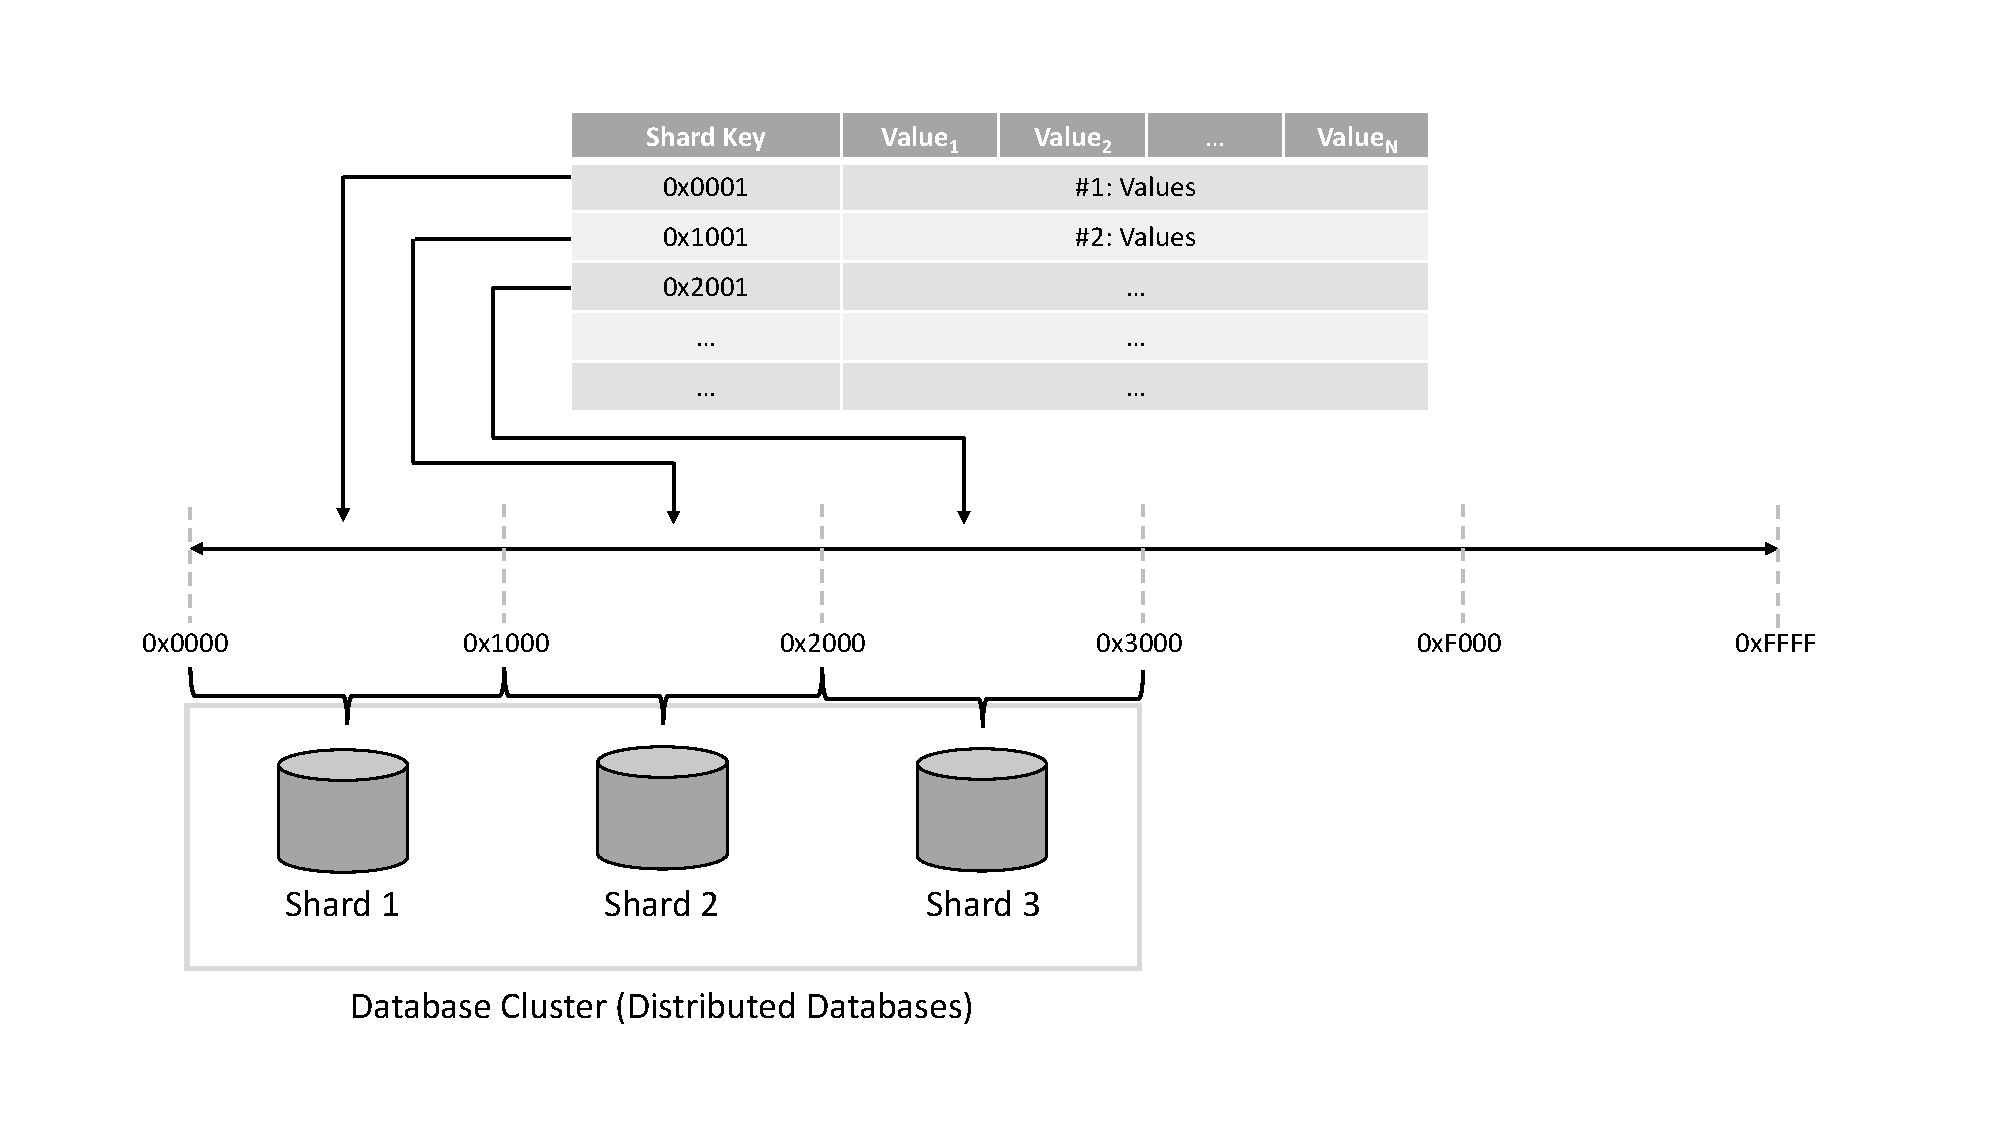
\includegraphics[scale = 0.4]{gfx/design/range_sharding.pdf}}{\caption{Range-based Sharding}\label{range-shard}}
\end{figure}

\noindent This sharding may result in uneven data distribution and overload on a single database node, depending on the data values \cite{Harrison2021, 10.14778/2556549.2556572}. 
In the prior example, the range of values with usernames starting from A to E might have much larger entries than the usernames from F to J. Despite these potential drawbacks, this method is relatively straightforward to implement.

\item \textit{Hash-based Sharding / Algorithmic Sharding} \\
In hash-based sharding, also referred to as algorithmic sharding, a hash function is employed to determine the database node for storing a specific data shard. The hash function accepts a key and generates a hash value (digest), and subsequently determines the data allocation node \cite{costa2015sharding, venkateswaran2017simplified}. \cref{hash-shard} shows an example of hash-based sharding approach. 

\begin{figure}[H]
             \ffigbox{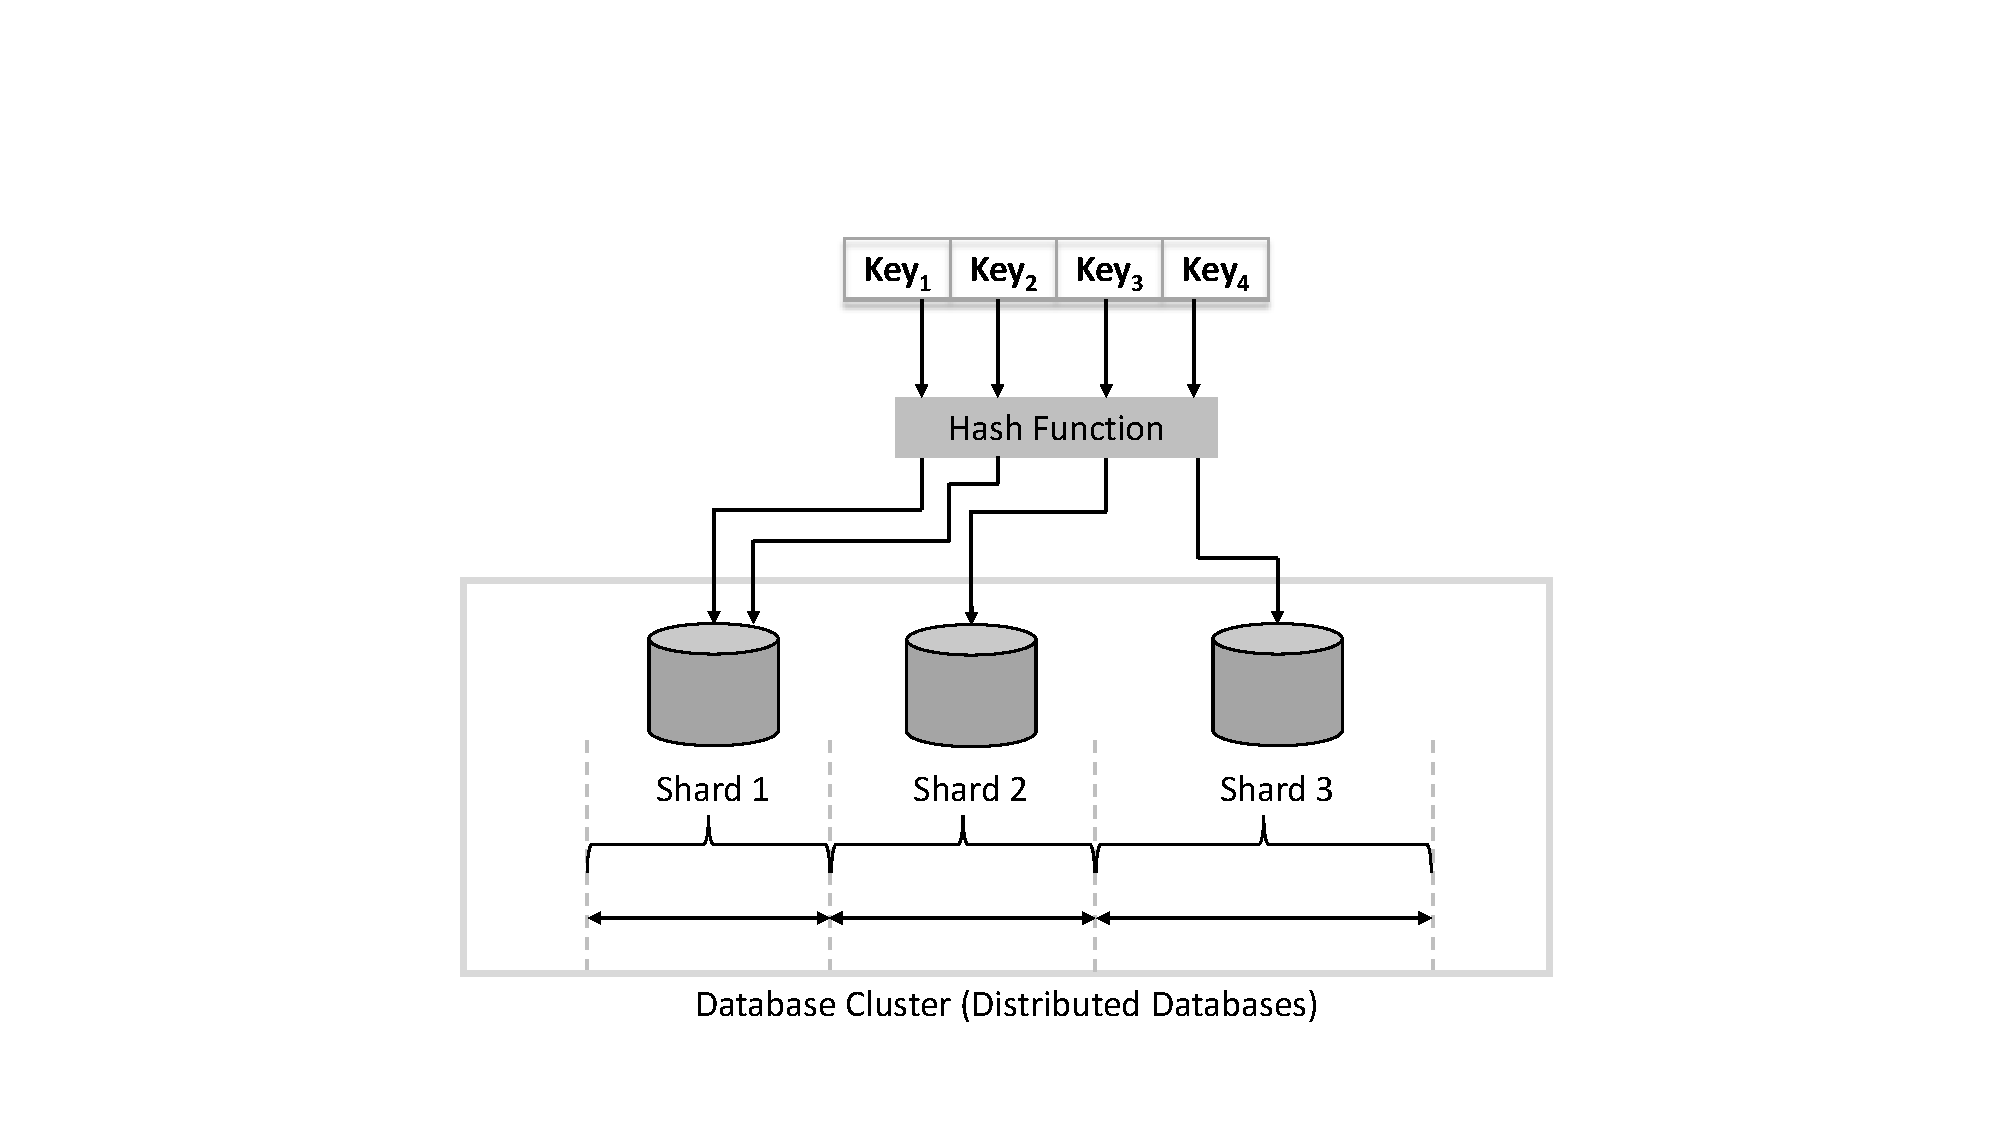
\includegraphics[scale = 0.4]{gfx/design/hash_sharding.pdf}}{\caption{Hash-based Sharding}\label{hash-shard}}
\end{figure}

\noindent Hash-based sharding is favorable when the data lacks a natural key range, and even distribution across sites is crucial. Although this approach ensures uniform data distribution among associated database nodes, it does not shard the data according to any semantically meaningful attributes.

\item \textit{Geo Sharding / Zone-based Sharding} \\
Geo-based sharding or zone-based sharding is a location-aware sharding approach, where data is partitioned based on a user-defined criteria that maps range of data to specific geographical regions and database nodes within those regions. The primary motivation for geo-based sharding is to place data closer in perimeter, both in terms of location and network proximity, to the users and the applications requiring that data \cite{10.1145/2433396.2433424}. Essentially, this method constitutes a range-based sharding, wherein the shard key contains geographic information and the shards themselves are geolocated. For instance, in a dataset feature a "location" field for each entry, performance and system latency can be enhanced by creating a shard for each country or region and storing the corresponding data on that shard \cite{9989965}. \cref{zone-shard} gives an overview of zone-based sharding approach. 

\begin{figure}[H]
             \ffigbox{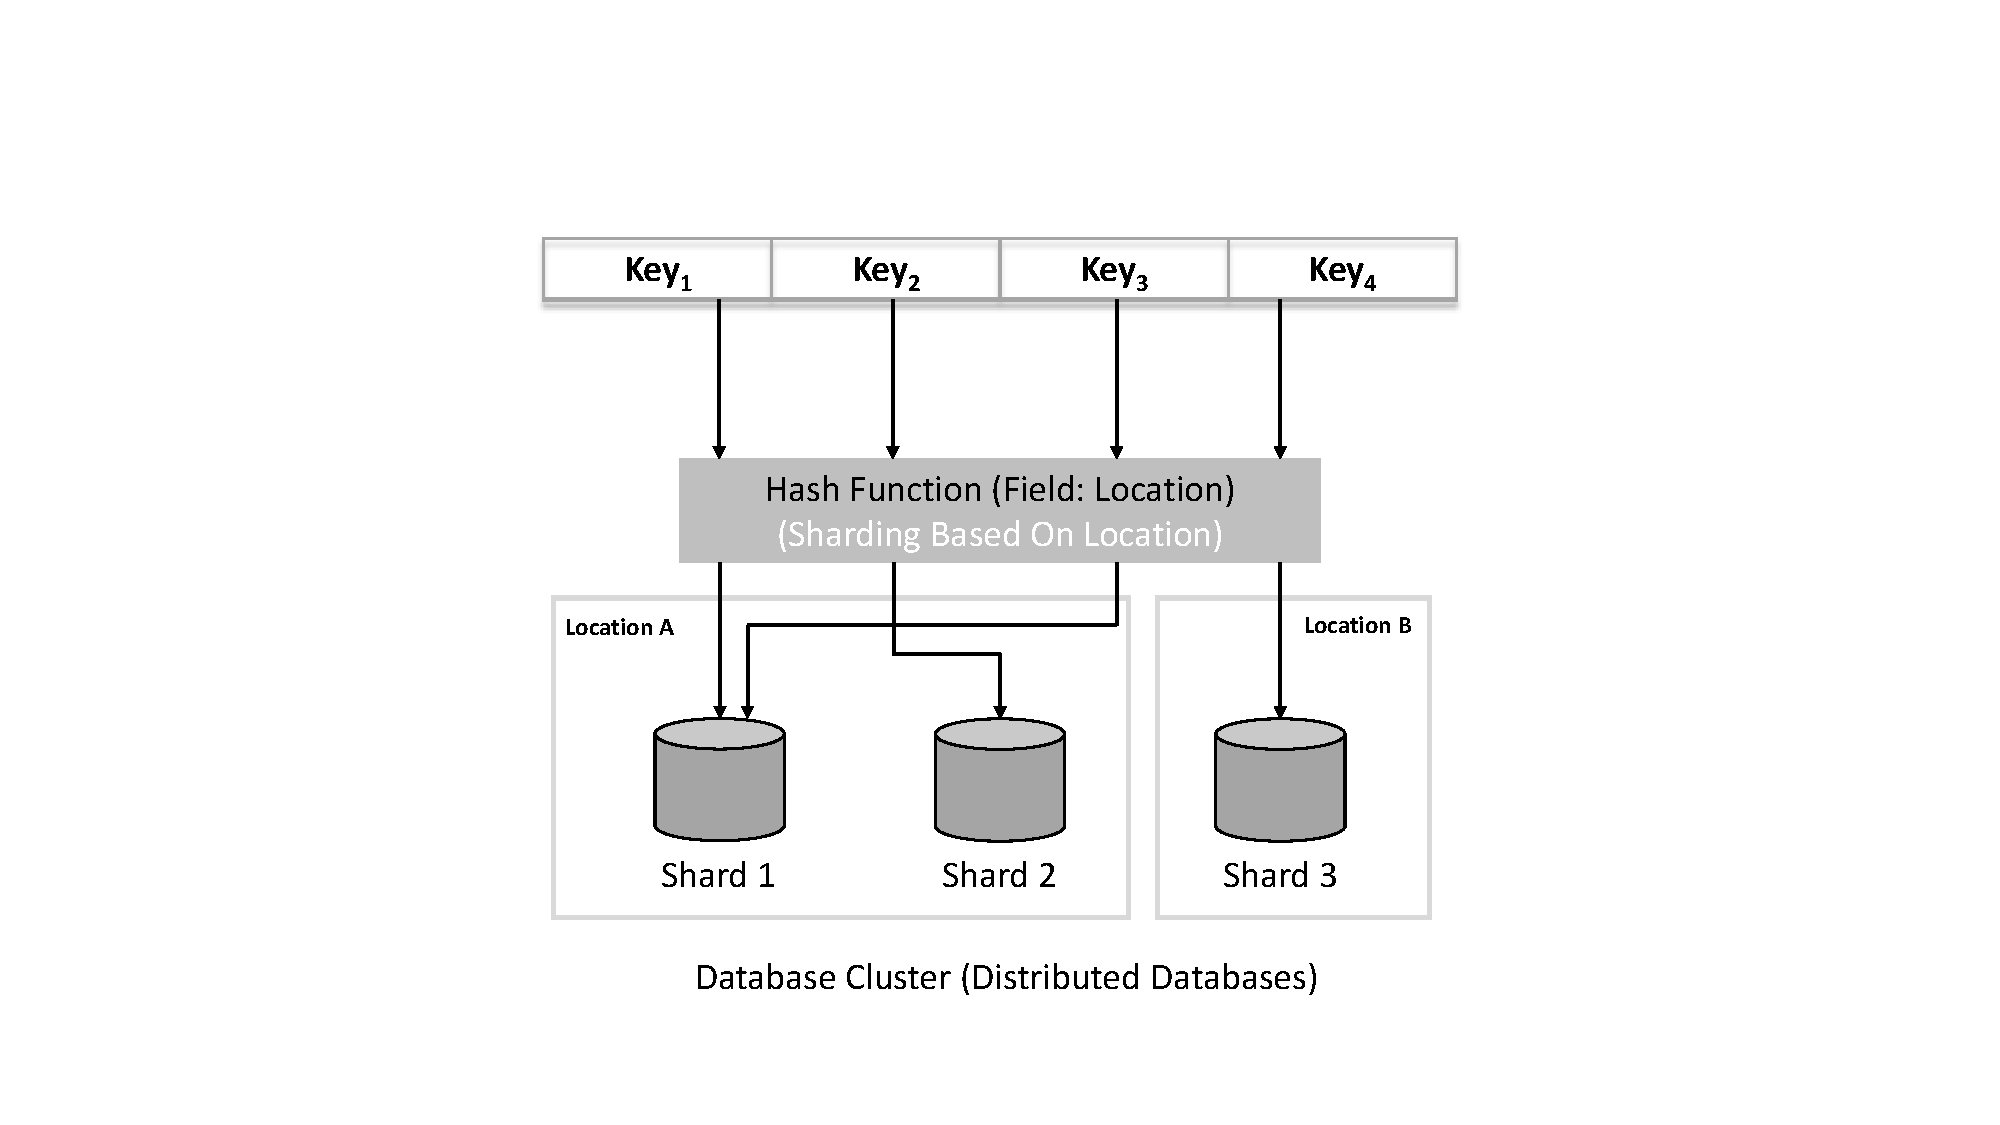
\includegraphics[scale = 0.4]{gfx/design/zone_sharding.pdf}}{\caption{Geo / Zone-based Sharding}\label{zone-shard}}
\end{figure}

\noindent Geo-based sharding proves particularly effective when data access patterns are predominantly based on geography. By partitioning data according to geographic regions or other location-related criteria, this approach offers advantages when it is crucial to store data closer to the users or applications that access it. Nevertheless, geographic-based sharding may lead to imbalanced data distribution across the system, as certain locations may have a higher concentration of users and data flow than others.

\item \textit{Entity-/Relationship-/Directory-based Sharding} \\
This approach utilizes a directory service or lookup table to map data to their corresponding shards, offering flexibility in data distribution and the potential for re-sharding with minimal impact \cite{9357711}. A lookup table holds information about where specific data can be found and, in this context, it uses a shard key to track which shard holds which data. Upon receiving a request for specific data, the appropriate site, i.e., the entry for associated database node in the directory is retrieved based on the shard key. This approach is useful when the number of sites or data distribution is expected to change frequently and when related data must be consolidated within a single physical shard. \cref{directory-shard} illustrates an example of the range-based sharding employed in database systems.

\begin{figure}[H]
             \ffigbox{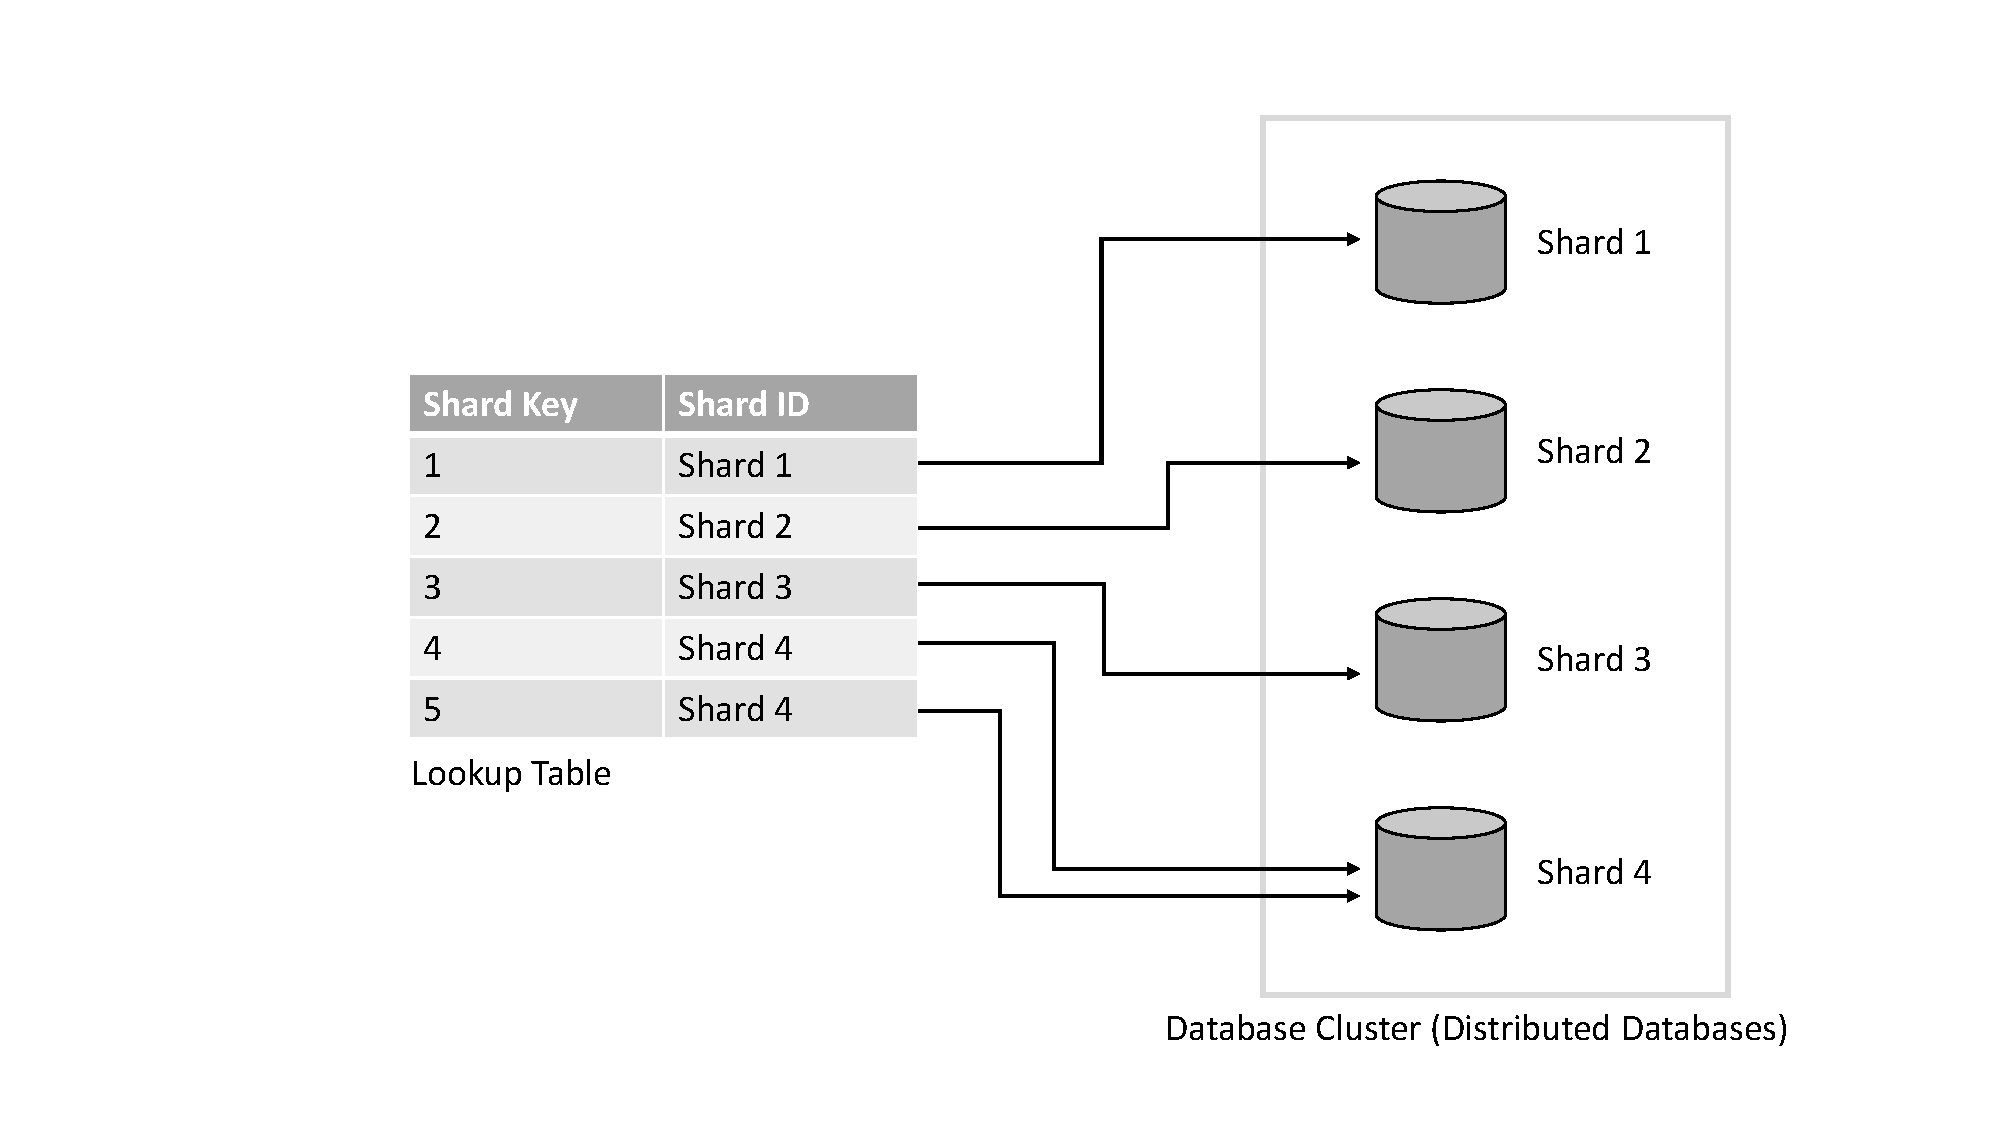
\includegraphics[scale = 0.4]{gfx/design/directory_sharding.pdf}}{\caption{Directory-based Sharding}\label{directory-shard}}
\end{figure}

\item \textit{Multi-level Sharding} \\
This method involves multiple levels of sharding based on data requirements, for instance, data may initially be sharded or partitioned by range, followed by the use of hashing on each key within each range \cite{chen2019sschain}. Multi-level sharding is suitable when scaling the system beyond the capabilities of a single sharding level is essential. 
However, it also introduces added operational complexity and computational overhead. As a result, careful design and planning are essential when implementing this approach.

\end{enumerate}

%***************************************************************************
\section{Related Works}
\label{2.4}
Traditional non-sharded database, typically deployed on a single database server, often becomes a bottleneck for scalability as data and requests increase \cite{schall2015dynamic}. When a single database server is insufficient for handling exceptionally large datasets or extremely high query throughput, sharding, often referred to as partitioning, becomes necessary \cite{ozsu1991distributed}. \\

\noindent Sharding enables distribution of data and query load across multiple database nodes, when processing data on a single database server is no longer feasible. This technique of sharding data and leveraging multiple database servers to process small data partitions or shards in parallel has led to the development of distributed databases \cite{ceri1987distributed}. Numerous works have been carried out on sharding and distributed databases to address the scalability bottleneck and performance issues associated with single database in the face of ever-growing data. New approaches and technologies for better sharding techniques and distributed databases continue to be researched and designed. 
INGRES \cite{stonebraker1976distributed} and SDD-1 \cite{rothnie1980introduction} marked the beginning of distributed databases and introduced the approach of splitting data among multiple database servers, which is a significant step in the evolution of sharded distributed databases. This development implied that distributed databases would provide more write bandwidth and higher availability. Each shard of data would be smaller than the full large dataset, making it faster to backup, recover, and manage. \\

\noindent Sharded databases with shared-nothing architecture were again pioneered in the late 1970s by Teradata, Tandem NonStop SQL, Bubba, and Gamma database systems \cite{stonebraker1986case, KAMAL2016421}. More recently, these concepts have been rediscovered in the era of big data and blockchain technology. Sharded Distributed databases now aim for horizontal scaling or scaling out to address reliability, availability, maintainability, and performance issues, which further solidifies the importance of sharding in modern data management \cite{dewitt1992parallel, mcsherry2015scalability}. \\

\noindent Various sharding algorithms have been proposed in the past, including consistent hashing \cite{karger1997consistent}, range partitioning \cite{curino2010schism}, and directory-based partitioning \cite{mahmud2020survey}.
Recent examples of sharded distributed databases include MongoDB \cite{mongodb}, Amazon DynamoDB \cite{sivasubramanian2012amazon}, Apache Ignite \cite{ignite}, Apache HBase \cite{hbase}, Couchbase \cite{couchbase}, FoundationDB \cite{foundation}, etcd \cite{etcd}, Redis \cite{redis}, Google's Cloud Spanner \cite{spanner}, CockroachDB \cite{cockroach}, etc. These databases employ different sharding strategies and techniques to ensure optimal performance, scalability, and data management in distributed systems. Sharding terminology does indeed vary across many state-of-the-art distributed databases. MongoDB, Elasticsearch \cite{elasticsearch}, and SolrCloud \cite{solrcloud} use the term "shard”, Apache HBase uses "region”, Google’s Bigtable \cite{chang2008bigtable} uses "tablet”, Cassandra \cite{cassandra2014apache} and Riak \cite{klophaus2010riak} use "vnode", and Couchbase uses "vBucket." Despite the differences in terminology, all these terms fundamentally represent blocks or chunks of data derived from a large dataset. \\

\noindent Google's Cloud Spanner \cite{spanner} and Apache Cassandra \cite{cassandra2014apache} are notable examples of sharded distributed databases that have made significant contributions to the field. Both databases have been designed with scalability, high availability, and distributed data management in mind, making them well-suited for handling big data.
Google's Spanner is a globally distributed database that shards data across multiple sets of Paxos state machines \cite{corbett2013spanner}. It offers high availability and geographic locality by sharding data and migrating it across machines to balance the load and respond to failures. Apache Cassandra, inspired by the range sharding of Google's Bigtable and the consistent hash sharding of Amazon's DynamoDB, is a popular distributed database choice for big data management \cite{chebotko2015big}. It ensures zero downtime, linear scalability, and seamless deployment across multiple data centers. Cassandra adopts a linear hash sharding approach, which is a hybrid of range and consistent hash sharding methods. Both Spanner and Cassandra have significantly advanced the field of sharded distributed databases, highlighting how these systems can effectively handle large-scale data management challenges with resilience, scalability, and performance. \\

\noindent Sharding approaches also play a vital role to enhance the performance of search engines, by helping to distribute data and workload across multiple database servers, enabling more efficient parallel processing and faster query response times \cite{DHULAVVAGOL20201626}. The primary goal of search engines is to refine user queries and retrieve only relevant documents from the appropriate shards while disregarding irrelevant data from other shards \cite{mohammad2018dynamic}.
In \cite{elasticShard} different sharding techniques are implemented and evaluated using the Elasticsearch platform, a widely used search and analytics engine. The objective is to develop a mechanism that can handle large-scale data processing and searching operations effectively through efficient sharding techniques. \\

\noindent Sharding is also used for achieving scalable blockchains, as it addresses the inherent limitations of existing blockchain systems, such as low transaction throughput, long confirmation times, and increasing storage requirements \cite{croman2016scaling}. These challenges stem from the fact that every node in a traditional blockchain network stores and processes the entire transaction history, leading to inefficiencies as the network size grows \cite{zamani2018rapidchain}. In blockchain systems, sharding is employed to divide the network into smaller, manageable partitions or shards. Each shard processes a subset of transactions independently, thereby increasing overall throughput and reducing the storage and processing burden on individual nodes. This approach allows for the parallel processing of transactions and enhances the network's scalability. Several new protocols have been developed to use sharding as part of the blockchain consensus protocol to address the scalability challenge of blockchains \cite{sonnino2018chainspace, kokoris2018omniledger, zamani2018rapidchain}.






\iftoggle{parts}{
	\cleardoublepage
	\ctparttext{The contribution starts with a design chapter, where we mathematically describe the design of the physical layer security system, as well as the adaptive filter of the attacker. After the design follows the implementation on WARP nodes. Here we give an insight into the challenges of implementing the designed MIMO communication system. The last chapter concentrates on evaluating the performance of our proposed attack in simulation and practice.}
	\part{Contribution}
}{}
%% !TeX root = ../Thesis.tex

%************************************************
\chapter{Sharded Distributed Databases}\label{ch:ShardedDistributedDatabases}
%************************************************
%%\glsresetall % Resets all acronyms to not used
\section{Sharding Strategies}

Database sharding splits a large dataset from a single database node into multiple shards. Each shard contains unique information that one can store separately across multiple database sites. A single site can contain multiple shards. Although the shards are distributed over multiple sites, they share the original database’s schema or design. Before sharding, one should determine a shard key to partition the dataset. Shard key determines which data are grouped together. Shard key is, either selected from an existing key in the dataset or created based on the properties of the existing data. 

Approaches for sharding databases:
Database sharding methods apply different rules to the shard key to determine the correct site for a particular set of data.

\begin{enumerate}
\item Range-based Sharding (Dynamic sharding):

In range-based sharding, data is partitioned based on a key range. For example, data for all users with user IDs between 1 and 1000 might be stored on one site, while data for users with IDs between 1001 and 2000 might be stored on another site. This type of sharding is useful when the data can be easily partitioned based on a specific key range. Depending on the data values, range-based sharding can result in the overloading of data on a single site, resulting an uneven distribution of data. In the preceding example, the first shard with user IDs between 1 and 1000, might contain a much larger amount of data than the second shard with user IDs between 1001 and 2000. However, this approach is easier to implement.

\item Hashed-based Sharding (Algorithmic Sharding):

In hash-based sharding, a hash function is used to determine which site, a piece of data (shard) should be stored in. The hash function takes a key (such as a user ID) as input and produces a hash value that is used to determine which site the data should be stored on. This type of sharding is useful when the data does not have a natural key range and when it is important to evenly distribute the data across the sites. Although hashed-based sharding results in even data distribution among physical shards, it does not partition the database based on the meaning of the information. Therefore, one might face difficulties reassigning the hash value when adding more physical shards to the computing environment.

\item Geo Sharding (Zone-based sharding): 

In zone-based sharding, data is partitioned based on geographic regions or other criteria related to locations. This type of sharding is useful when it is important to store data closer to the users or applications that will access it. If data access patterns are predominantly based on geography, then this works well. However, geo sharding can also result in uneven data distribution.

\item Entity-/Relationship-based/Directory-based Sharding:

In directory-based sharding, a central directory is used to map keys to nodes. When a client wants to store or retrieve data, it looks up the appropriate site in the directory based on the key. This type of sharding is useful when the number of sites or the data distribution is likely to change frequently. This approach also keeps related data together on a single physical shard.

\item Multi-level sharding:

In multi-level sharding, data is partitioned using multiple levels of sharding. For example, data might be first sharded by range and then further partitioned by hash within each range. This type of sharding can be useful when it is important to scale the system beyond what is possible with a single level of sharding.
\end{enumerate}

\section{Sharded Data Distribution}

When a data overload occurs on specific physical shards although others remain underloaded, it results in database hotspots. Hotspots slow down the retrieval process on the database, defeating the purpose of data sharding. 
Good shard-key selection can evenly distribute data across multiple shards. When choosing a shard key, database designers should consider the following factors:
\begin{itemize}
\item Cardinality: Cardinality describes the possible values of the shard key. It determines the maximum number of possible shards on separate column-oriented databases. For example, if the database designer chooses a yes/no data field as a shard key, the number of shards is restricted to two.
\item Frequency: Frequency is the probability of storing specific information in a particular shard. For example, a database designer chooses age as a shard key for a fitness website. Most of the records might go into nodes for subscribers aged 30–45 and result in database hotspots.
\item Monotonic change is the rate of change of the shard key. A monotonically increasing or decreasing shard key results in unbalanced shards.
\end{itemize}

\section{Distributed Transaction and Query Processing}
\section{Distributed Concurrency Control}
\section{Distributed Recovery}


% !TeX root = ../Thesis.tex

%************************************************
\chapter{Design}\label{ch:design}
%************************************************
%%\glsresetall % Resets all acronyms to not used
This section presents the design principles and considerations for implementing a middleware-assisted system of sharded distributed databases. The subsection \ref{sys_design} describes the middleware's design, detailing its functionalities and various interacting components, including associated distributed databases and clients. Meanwhile, the subsection \ref{sys_design_limits} addresses the scope and limitations of the middleware's design.
%##############################################
\section{System Design of Sharded Distributed Database}
\label{sys_design}
In designing a system for sharded distributed databases, this thesis proposes the use of middleware as a software layer responsible for coordinating the execution of client requests across one or more independent database servers. The system comprises three types of components that interact with each other: clients, a single instance of the middleware, and multiple database servers.


\begin{figure}[H]
             \ffigbox{
\includegraphics[scale = 0.45]{gfx/design/mware_design.pdf}}{\caption{Middleware Design (Abstract Overview)}\label{m_design}}
\end{figure}

\subsection{Middleware’s Design and Components}
The middleware serves as an intermediary between clients and multiple database servers without storing any data itself. It implements a sharding algorithm to facilitate a system of distributed databases. The middleware is responsible for coordinating multiple databases and offering a single, unified interface for clients. It processes all client requests, helping in data sharding and distributing the associated data across relevant databases. Furthermore, it manages data distribution and distributed queries, aggregating partial results from multiple databases to generate the desired response for each request. By providing a consistent interface for interacting with databases, the middleware effectively conceals the underlying functionalities and separation of databases from clients. Consequently, clients perceive their interactions as if they were accessing a single database entity.
Considering the outlined requirements, the middleware is divided into the following modules or components:


\begin{enumerate}

\item Service Listener: \\
The middleware 

\item Shard Management: \\
This module implements the sharding algorithm, which manages data and query/request distribution. It retrieves the URLs (Uniform Resource Locator) of associated database nodes based on the hashed key (shard key) and sharding algorithm. Additionally, it determines the initial placement of shards on database nodes while considering uniform data load balancing.

\item Database Communication Interface: \\
This interface serves as a vital connection between the middleware and the associated databases. It provides an interface for communication and manages the addition and removal of database nodes, also known as sites, as required during initial configuration. This component also initializes communication configurations with databases, including database identifiers, connection ports, and pools, and decodes responses received from the databases. Furthermore, it presents an interface for all database operation calls, such as set, get, update, and delete.

\item Query /Request Routing and Result Compilation: \\
This module is essential for processing client requests and generating appropriate responses. It breaks down a single client request into multiple sub-requests and sends them to the corresponding associated databases. This module then compiles and aggregates all partial results received from all associated databases and generates a single, valid response.


\end{enumerate}

%##############################################
\subsection{Distributed Databases}

%##############################################
\subsection{Client}
Client connects directly to the middleware, without knowing the specifications of underlying databases. The middleware exposes an Application Programming Interface (API) for setting, updating, retrieving/getting, scanning, and deleting single and multiple key-value pairs, which the client uses to send requests. Clients must perform all operations using the middleware's API. \\

\noindent Communication between the client and the middleware is implemented via the gRPC protocol. As a result, clients must implement a gRPC stub responsible for packaging the request in a Proto message format (serialization), sending the request to the middleware, and unpacking the received response from the middleware (deserialization) and decoding the response into a client-supported data format.


\begin{figure}[H]
             \ffigbox{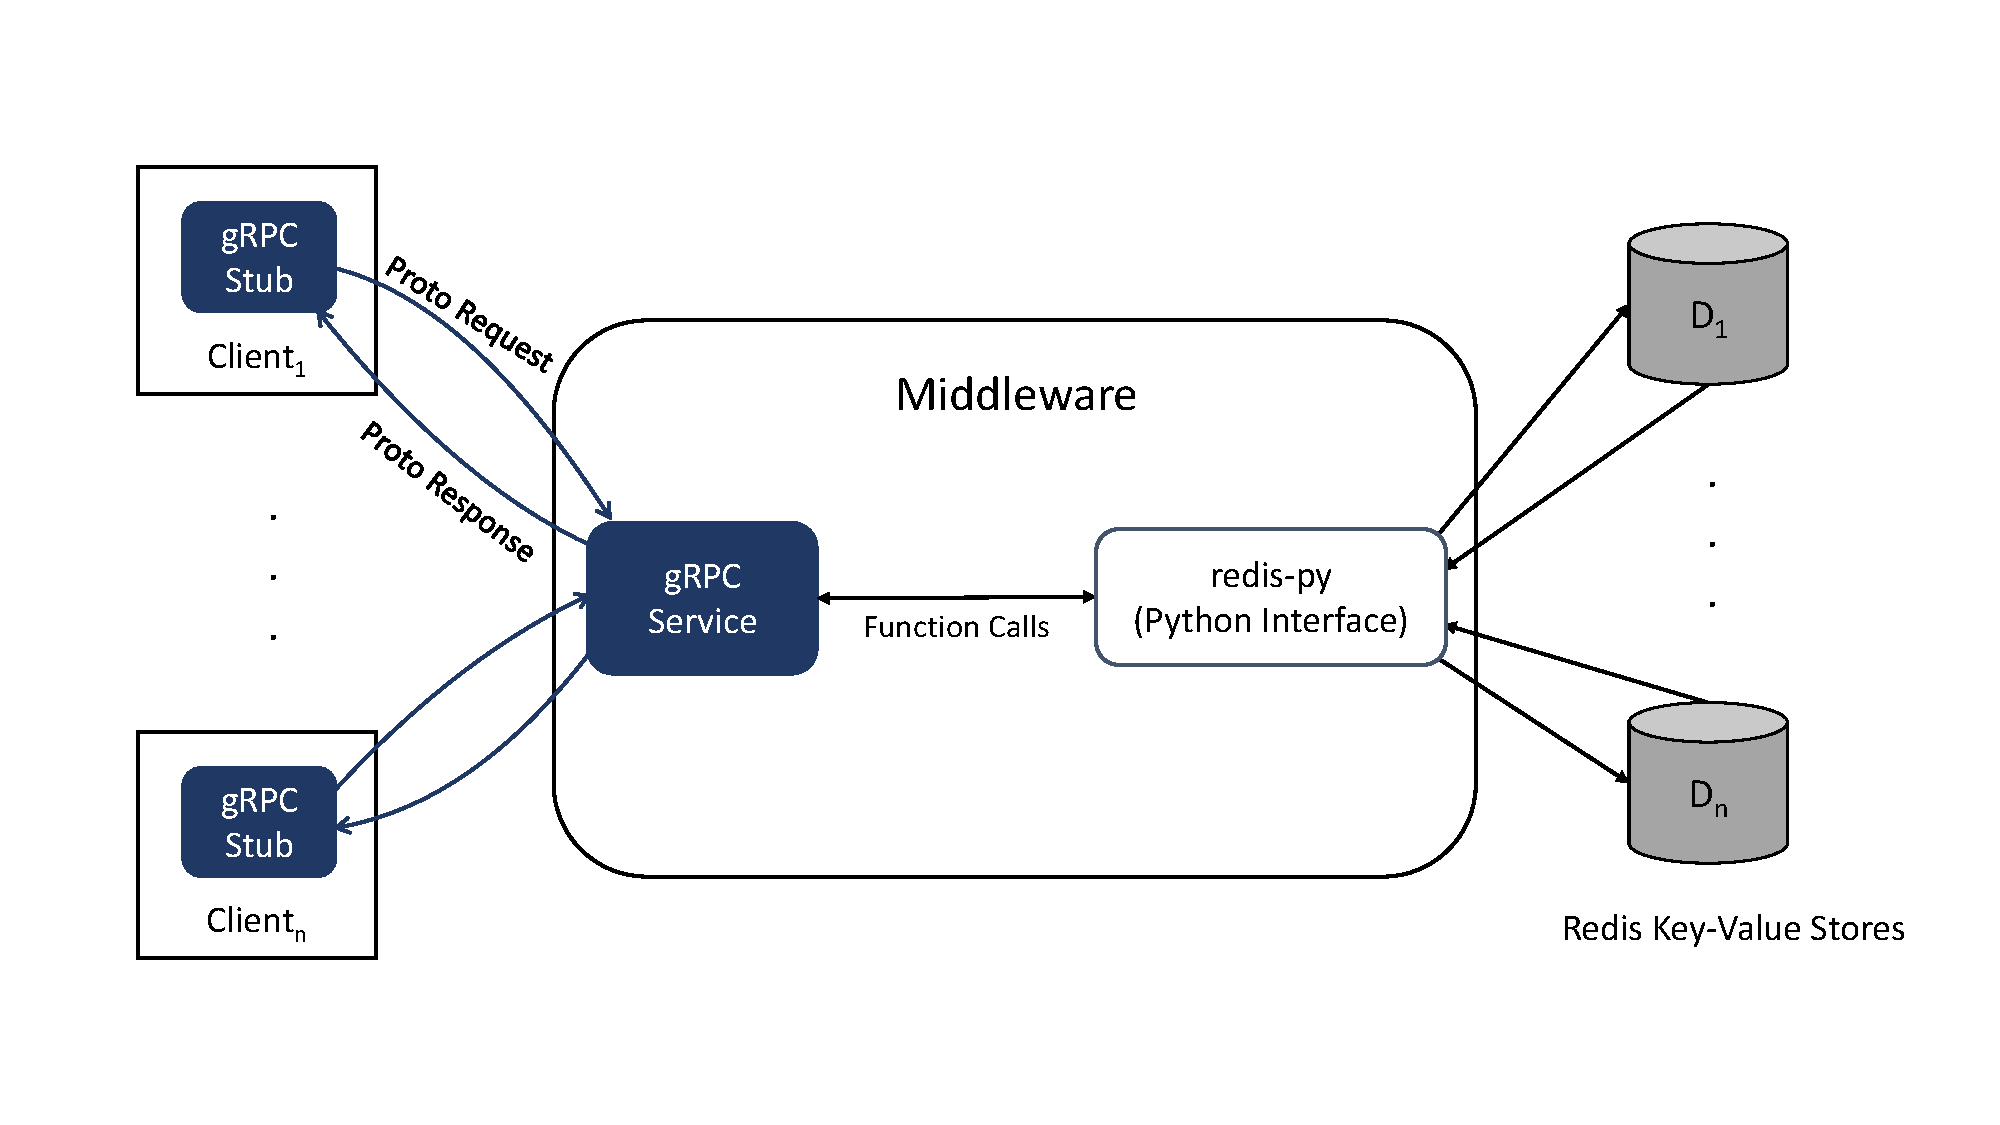
\includegraphics[scale = 0.45]{gfx/design/communication.pdf}}{\caption{Middleware Communication Overview}\label{communication}}
\end{figure}





%***************************************************************************
\section{Design Limitations}
\label{sys_design_limits}

%***************************************************************************

% !TeX root = ../Thesis.tex

%************************************************
\chapter{Implementation}\label{ch:implementation}
%************************************************
%%\glsresetall % Resets all acronyms to not used
%***************************************************************************
\section{Middleware Design and Architecture}


%***************************************************************************
\section{Operations}


%***************************************************************************
\section{Sharding in Redis Key-Value Stores}

% !TeX root = ../Thesis.tex

%************************************************
\chapter{Evaluation and Results}
\label{evaluation}
%************************************************
%\glsresetall % Resets all acronyms to not used
This section provides a comprehensive assessment and analysis of the middleware’s performance utilizing defined performance metrics of throughput and response time, custom workload, and custom benchmarking process. The middleware’s performance is evaluated across various test scenarios, featuring different middleware configurations based on the performance metrics introduced in the subsection \ref{performanceMetrics}. The performance with and without the middleware using the same workloads are compared applying the experimental setup and methodology outlined in the subsection \ref{setupMethod}. \\

\noindent Subsequently, the subsection \ref{throughputAnalysis} examines the impacts of configuration changes of the middleware on average throughput and average response time. From the generated test results, the average throughput and the average response time of the middleware are derived. Moreover, the results from the performance analysis are interpreted and investigated to identify anticipated bottlenecks and limitations in the middleware, and potential solutions for optimization are suggested. \\

\noindent Finally, the subsection \ref{throughputAnalysis} provides a brief overview of the nearly balanced data distribution among the Redis databases achieved through the middleware’s consistent hash sharding approach. 

%***************************************************************************
%***************************************************************************
\section{Performance Metrics}
\label{performanceMetrics}

\begin{figure}[H]
             \ffigbox{
\includegraphics[scale = 0.45]{gfx/figures/Baseline_Response_Latency.pdf}}{\caption[Illustration of latency, processing time and response time observed in baseline]{Illustration of latency, processing time and response time measured in the baseline for comparison}\label{latency_response_baseline}}
\end{figure}

\textbf{Latency} is the time duration between the initiation of a request transmission by a source and the reception of the corresponding message by the destination. Such latency manifests as the time in which the request is held in a waiting state prior to processing. Round-trip latency, whereas, is defined as time elapsed between the transmission of a request and the receipt of the corresponding response. It does not account for the processing time incurred at the destination. In the system architecture examined in this thesis, two types of latency require consideration. The first latency type involves round-trip latency occurring throughout the communication between the client and the middleware, while the second type pertains to round-trip latency in the interaction between the middleware and the associated Redis database instances. Both latencies are crucial for comprehending the overall performance of the proposed middleware and are measured in milliseconds (ms). \\

\noindent \textbf{Processing time} refers to the time taken by a processing system to execute a received request. It is computed as the time duration between the moment when the system receives the final byte of the request and the moment when it transmits the first byte of response. To evaluate the performance of the proposed system of sharded distributed databases, the processing time for all operations performed by the middleware is assessed. These processing times enclose the time taken for decomposing requests from the client into multiple sub-requests, sharding associated data and allocating it to appropriate Redis database, constructing pipelines to transmit the sub-requests to appropriate shards, merging the received partial results from the involved Redis databases and aggregating these partial results to generate a corresponding response to the initial request. The processing time for the middleware is measured in milliseconds (ms). \\

\noindent \textbf{Response time} of the examined system is the total time elapsed from the initiation of a request transmission to the receipt of the corresponding response, measured in milliseconds (ms). It represents a cumulative time duration, comprising both the latency and internal processing time of the entire system. For the evaluation, two average response times are measured. The first measurement, i.e., the average response time of the baseline, is obtained from the client-side when connected directly to a single Redis database without the middleware. The second measurement is the average response time observed from the client when connected to the middleware. Comparing these average response times provides valuable insights into the performance impact of the middleware on the system. \\

\noindent \textbf{Throughput} is a performance metric, which quantifies the total number of requests that a system can successfully process within a given time. In the context of this evaluation, the middleware’s throughput is thoroughly examined, as it is responsible for handling all incoming client requests. The middleware’s throughput is expressed in Requests Per Second (RPS). Factors influencing the throughput of the middleware include computing resources of the host machine on which the middleware is installed, the processing overhead associated with the middleware, the degree of parallelism or concurrency within the middleware and the types of requests the middleware processes. To facilitate a comparison, the average throughput of the baseline, i.e., a single Redis database employing the same workload as the middleware, is measured.
The workload employed for evaluating response time and throughput is interpreted in the subsection \ref{workloadBenchmark}. \\

\noindent The observed latencies, processing times, and response times in the baseline for comparison are illustrated in \cref{latency_response_baseline}, while those for the middleware-assisted sharded distributed databases are depicted in \cref{latency_response}.

\begin{figure}[H]
             \ffigbox{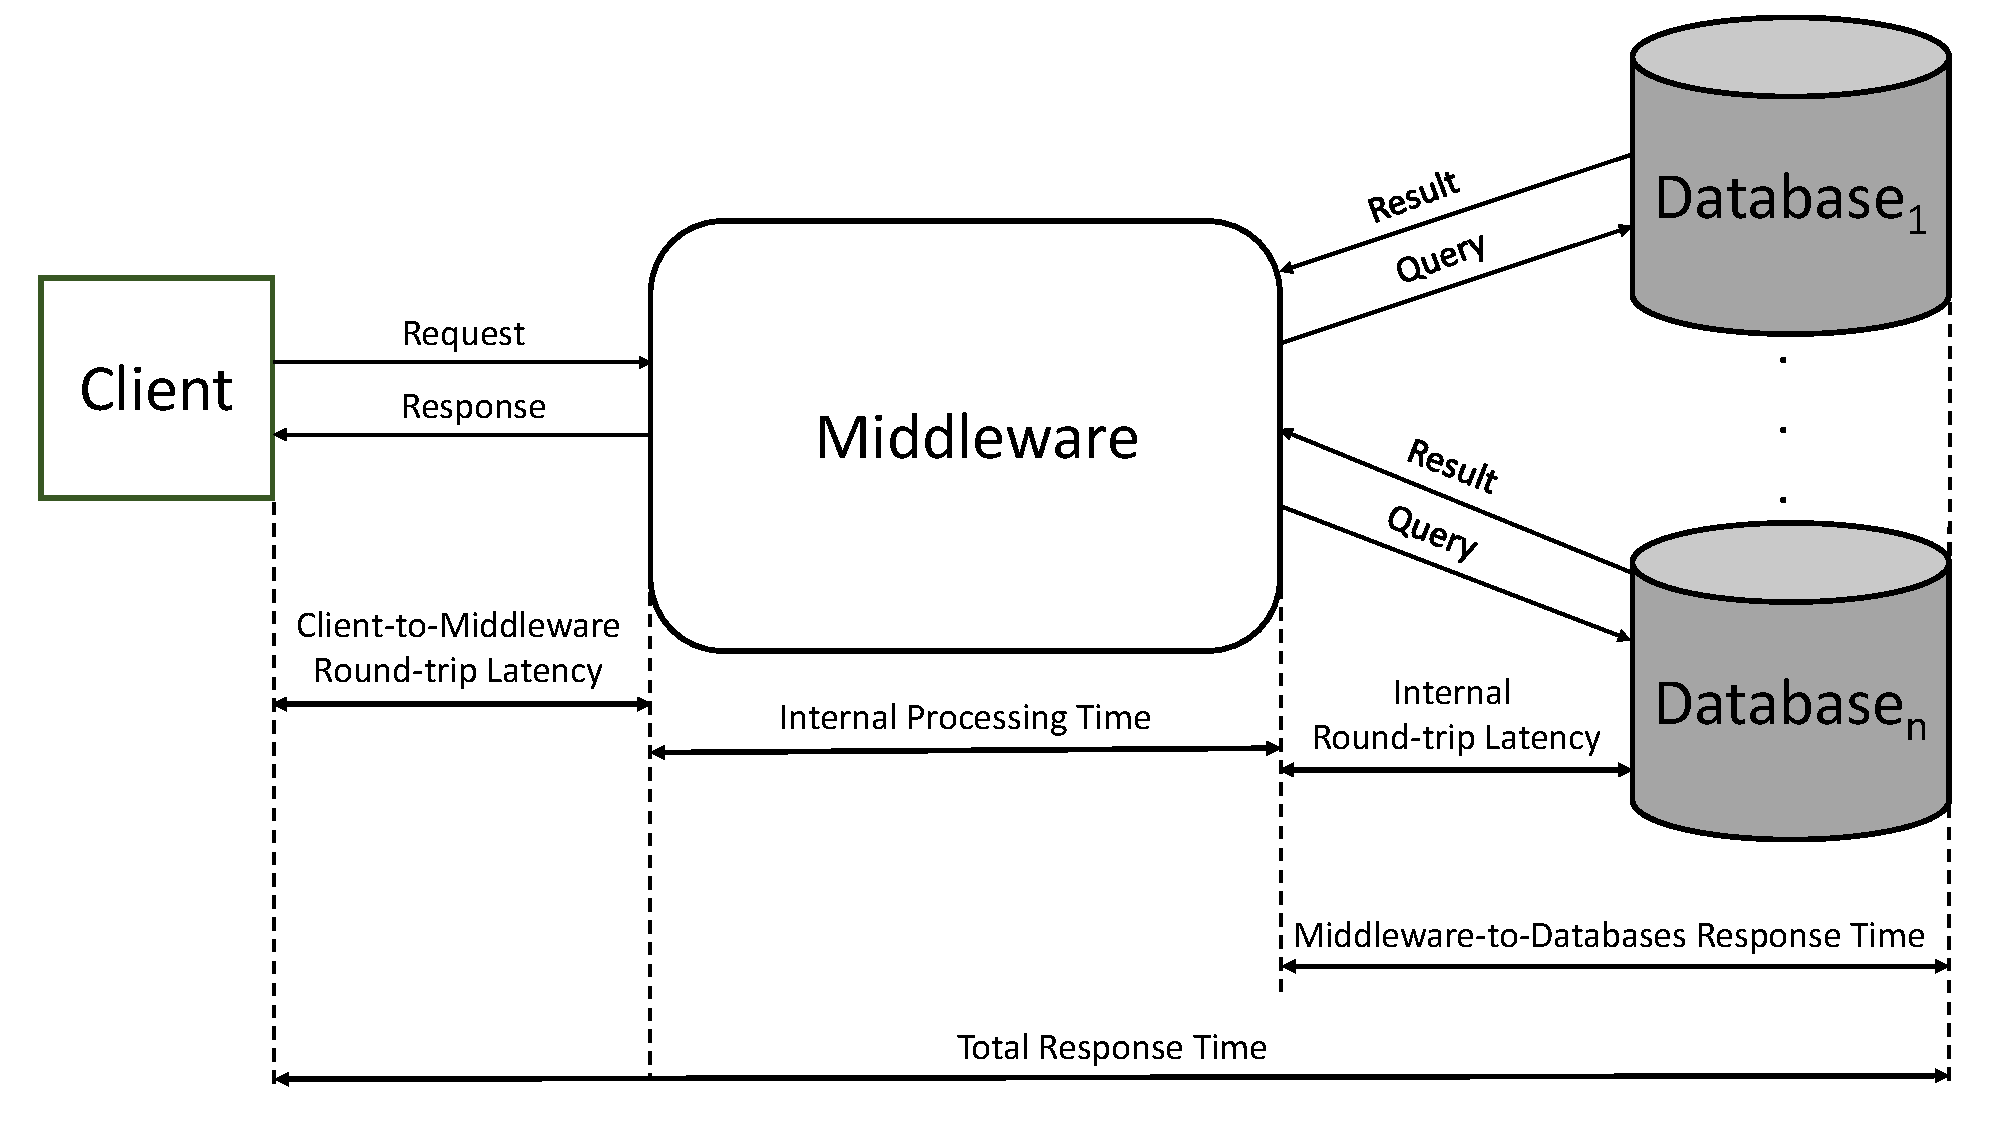
\includegraphics[scale = 0.45]{gfx/figures/Latency_Response_M.pdf}}{\caption[Illustration of observed latencies, processing time and response times in middleware-assisted sharded distributed databases]{Comprehensive illustration of latencies, processing time and response times measured in the proposed system of middleware-assisted sharded distributed databases}\label{latency_response}}
\end{figure}

%\begin{figure}[H]
%             \ffigbox{
\includegraphics[scale = 0.45]{gfx/reports/Report_3_18_2023_4_19_pm.pdf}}{\caption{Performance evaluation of the middleware through benchmarking, where a load of 100 concurrent clients are generated progressively at the rate of 10 clients per second}\label{benchmark}}
%\end{figure}
%%%%%%%%%%%%%%%%%%%%%%%
\begin{comment}   
\begin{figure}[H]
	\begin{floatrow}
             \ffigbox{
\includegraphics[scale = 0.5]{gfx/visualizations/set.pdf}}{\caption{Set Key-Value Pairs}\label{set}}
             \ffigbox{
\includegraphics[scale = 0.5]{gfx/visualizations/get.pdf}}{\caption{Get Key-Value Pairs}\label{get}}
	\end{floatrow}
\end{figure}
\begin{figure}[H]
	\begin{floatrow}
             \ffigbox{
\includegraphics[scale = 0.5]{gfx/visualizations/get-range.pdf}}{\caption{Get Range Of Key-Value Pairs}\label{getRange}}
             \ffigbox{
\includegraphics[scale = 0.5]{gfx/visualizations/delete.pdf}}{\caption{Delete Key-Value Pairs}\label{delete}}
	\end{floatrow}
\end{figure}

\begin{figure}[H]
             \ffigbox{
\includegraphics[width=\textwidth]{gfx/visualizations/combined_visualization.pdf}}{\caption{Average response time per given key-value pairs of all functions provided by middleware}\label{combined}}
\end{figure}

\end{comment}
%%%%%%%%%%%%%%%%%%%%%%%

%***************************************************************************
%***************************************************************************
\section{Experimental Setup and Methodology}
\label{setupMethod}
In this subsection custom workload and benchmarking process are devised to conduct tests with concrete configurations and evaluate the middleware’s performance across different test scenarios.

%***************************************************************************
%***************************************************************************
\subsection{Custom Workload and Benchmarking Process}
\label{workloadBenchmark}
This study uses a custom workload consisting of two distinct datasets, $Dataset_{1}$ and $Dataset_{2}$, to evaluate the performance of the middleware-assisted sharded distributed databases. $Dataset_{1}$, the larger of the two, comprises 1000 key-value pairs, whereas the smaller dataset, $Dataset_{2}$ contains 100 key-value pairs. Each key within these datasets is a randomly generated 4-digit integer, which is associated with a value holding 3 distinct key-value pairs. The associated values consist of the key identifiers: $UserID$, $Name$, and $Email$. Among these key identifiers, $UserID$ serves as the shard key. The schema used in the datasets is exemplified with \cref{key-value-schema}. \\

\begin{figure}[H]
             \ffigbox{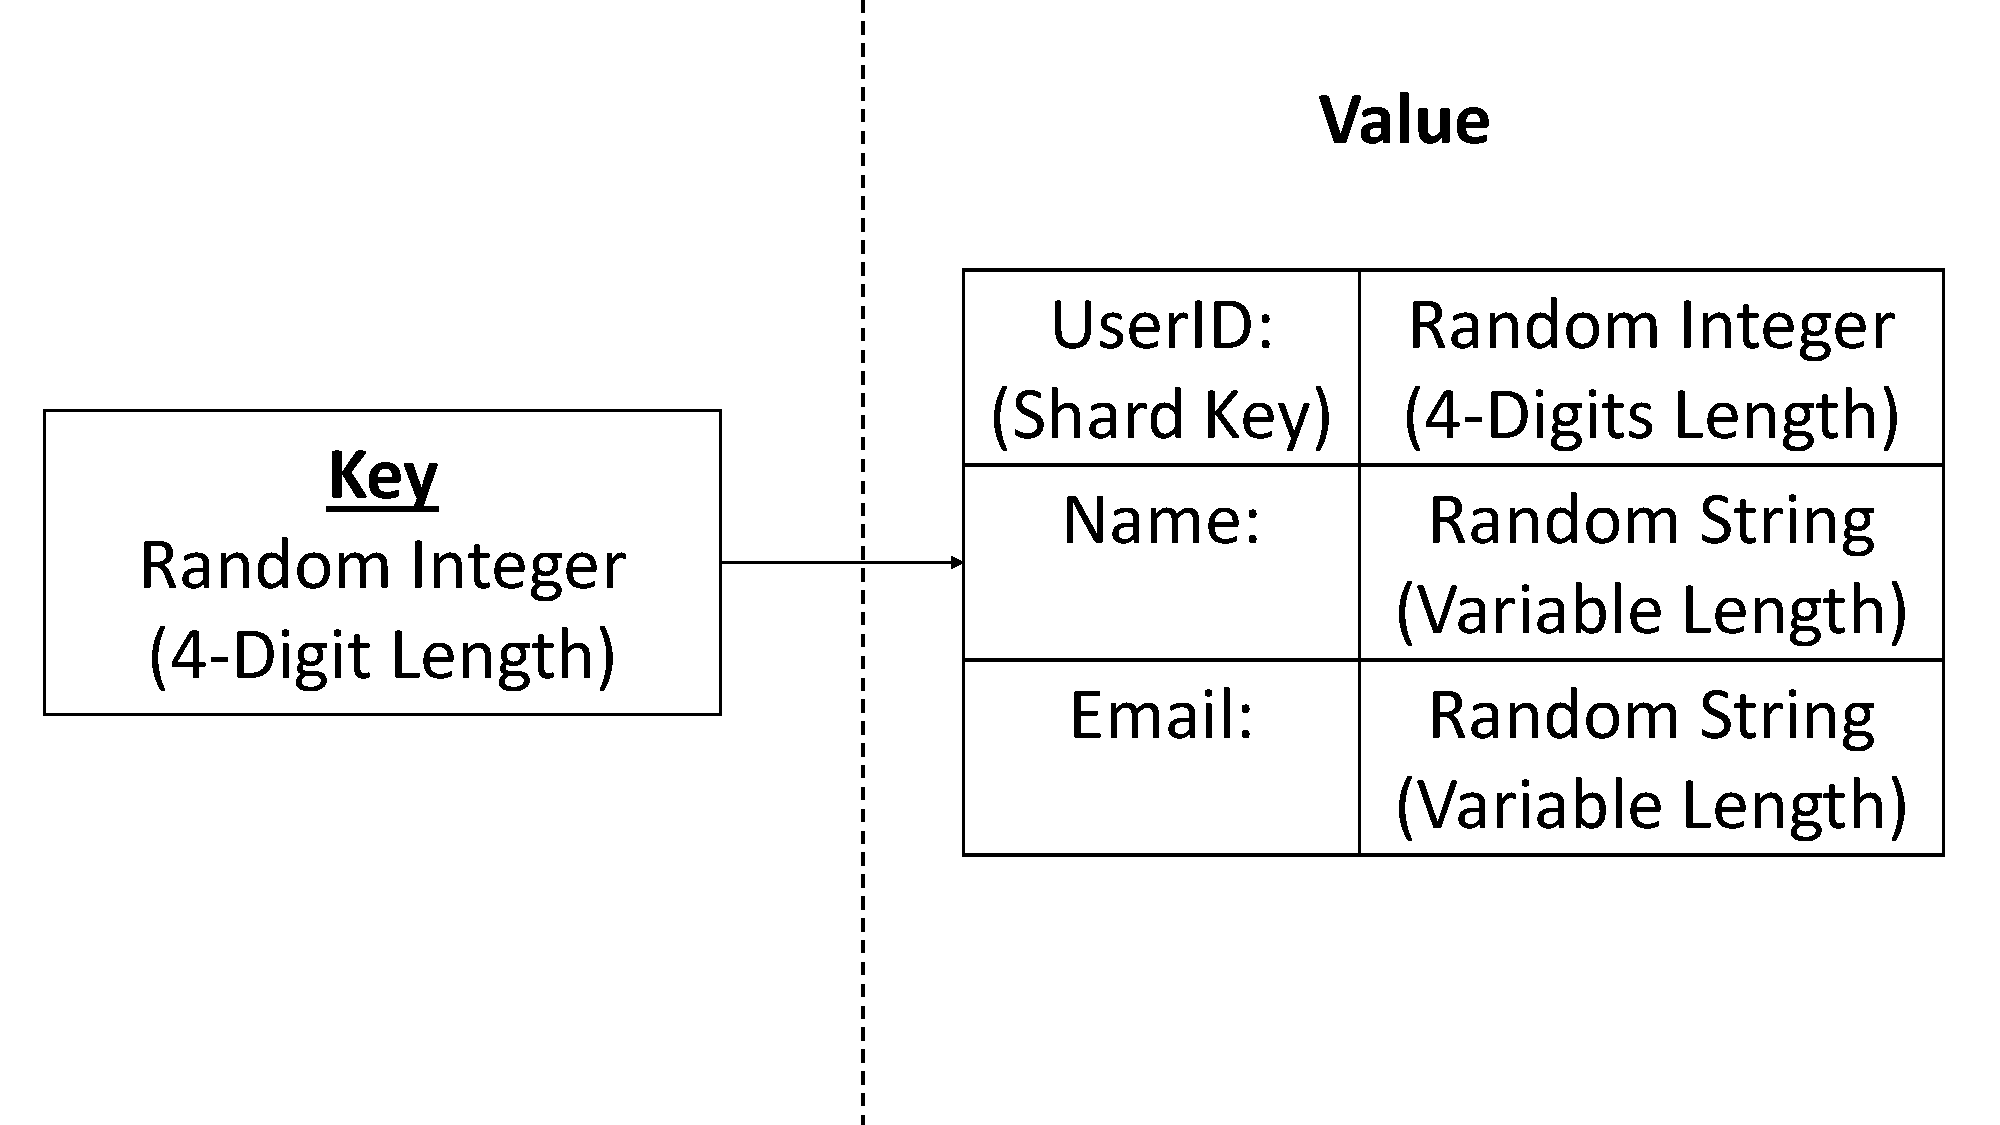
\includegraphics[scale = 0.25]{gfx/figures/workload_schema.pdf}}{\caption{Workload Schema}\label{key-value-schema}}
\end{figure}

\noindent    The custom benchmarking process evaluates the performance of various operations supported by the middleware using both $Dataset_{1}$ and $Dataset_{2}$. All operations use either single or multiple key-value pairs. To differentiate between the two, $Dataset_{1}$ is used for $set$, $get$, $get$-$range$, and $delete$ operations involving multiple key-value pairs, while $Dataset_{2}$ is used for $set$ and $get$ operations with single key-value pair. To simulate real-world scenarios with read-heavy and write-heavy operations, all 1000 key-value pairs from $Dataset_{1}$ are used for $set$ and $get$ operations with multiples key-value pairs. In contrast, only 100 keys are used for $get$-$range$ and $delete$ operations. For $set$, $get$, and $delete$ operations with single key-value pair, 1 randomly chosen key-value pair from $Dataset_{2}$ is employed. \\

\noindent \cref{tab:workload} presents a breakdown of the workload distribution for evaluating all specified operations of the middleware.
%You can find an example table in \cref{tab:workload} using the \emph{tabular} environment. Note the use of horizontal lines from the \emph{booktabs} package (\lstinline|\toprule|, \lstinline|\midrule|, and \lstinline|\bottomrule|) and removed whitespace at both sides of the table (\lstinline|@{}|) as proposed by Markus Püschel.\footnote{\url{https://www.inf.ethz.ch/personal/markusp/teaching/guides/guide-tables.pdf}}
%
\begin{table} [H]
\centering
\begin{tabular}{@{} lccr @{}} % @{} removes white spaces
	\toprule
	\tableheadlineL{Operations} & \tableheadline{Requests} & \tableheadline{Dataset} & \tableheadlineR{Tested Workload} \\ 
	\midrule
	\multirow{2}{*}{set} & set\textunderscore single & Dataset\textsubscript{2} & 1 Key-Value Pair \\
		& set\textunderscore multiple & Dataset\textsubscript{1} & 1000 Key-Value Pairs \\
	 \midrule
	\multirow{2}{*}{get} & get\textunderscore single & Dataset\textsubscript{2} & 1 Key-Value Pair \\
		& get\textunderscore multiple & Dataset\textsubscript{1} & 1000 Key-Value Pairs \\
	 \midrule
	get-range & get\textunderscore range & Dataset\textsubscript{1} & 100 Key-Value Pairs \\
	\midrule
	\multirow{2}{*}{delete} & del\textunderscore single & Dataset\textsubscript{2} & 1 Key-Value Pair \\
		& del\textunderscore multiple & Dataset\textsubscript{1} & 100 Key-Value Pair \\
	\bottomrule
\end{tabular}
% Use alternative short title for table of contents with \caption [SHORT-TITLE]
\caption{Workload distribution for tested operations}
\label{tab:workload}
\end{table}

\noindent To evaluate the middleware's average throughput and average response time, Locust  framework, a Python-based open-source load-testing tool, is utilized \cite{locust}. This tool simulates load of numerous concurrent clients on System Under Test (SUT), facilitating the analysis of the system’s behavior when subjected to high traffic from multiple concurrent clients. The load-testing is conducted under two distinct contexts. The initial context involves executing all operations directly on a single Redis database without the middleware, serving as the baseline configuration. This configuration adheres to the specified workload for the operations, as outlined in \cref{tab:workload}. In the subsequent context, the client is connected to the middleware, having different configurations as detailed in the subsection \ref{config}. In this context, all the operations with specified workload from \cref{tab:workload} are tested to gain insights about the middleware’s performance. \\

\noindent The middleware uses the Python module, \emph{logging} for generating internal logs and insights to measure the average processing time within the middleware and to determine the internal response time of connected Redis database instances to the middleware \cite{logging}. The \emph{timeit} Python module is used to estimate the execution time of the middleware for each operation over 1 million iterations \cite{timeit}. The return value is the average execution time in seconds. To measure the internal response time from the associated Redis databases within the middleware, the \emph{time.time()} function from the Python in-built module \emph{time} is used. This function returns the time since the Unix epoch, as a floating-point number expressed in seconds \cite{time}. For the custom benchmarking in this thesis, all values from the logs are converted to milliseconds (ms).


%***************************************************************************
%***************************************************************************
\subsection{System Configuration}
\label{config}
The middleware, the core component of the proposed sharded distributed databases, is the System Under Test (SUT). Every test scenario for performance evaluation is composed of one instance of middleware connected with varying number of Redis database instances. The number of client instances depends upon the test scenario. \\

\noindent The middleware and the Redis databases, used for the performance analysis are installed on separate machines, each with following specifications:
\begin{itemize}
\item[-] Processor: Intel(R) Xeon(R) Silver 4214R CPU @ 2.40GHz (24 CPU cores)
\item[-]  Memory: 32 GiB RAM
\item[-]  Operating System: Ubuntu 22.04.1 LTS
\end{itemize}
In contrast, each client machine is equipped with the following specifications:
\begin{itemize}
\item[-]  Processor: Intel(R) Core (TM) i5-9400F CPU @2.90GHz (6 CPU cores)
\item[-]  Memory: 8GiB RAM
\item[-]  Operating System: Windows 11 Home 64 bit
\end{itemize}

\noindent For testing and evaluation of the SUT, different parameters are considered, which are as follows:
\begin{itemize}
\item \textbf{Workload:} $Dataset_{1}$ and $Dataset_{2}$ as described in the subsection \ref{workloadBenchmark}. 
\item \textbf{Client-load:} It is the number of concurrent clients performing all operations ($set$, $get$, $get$-$range$, and $delete$) involving single and multiple key-value pairs. Depending upon the test scenario, the client-load remains constant or increases gradually with time throughout the test execution.
\item \textbf{Baseline:} It is the configuration where the client connects directly with 1 Redis database and performs all given operations without the middleware. It serves as a starting point for comparing and analyzing the performance of the middleware. The baseline tests are executed with the custom workload, $Dataset_{1}$ and $Dataset_{2}$.
\end{itemize}

\noindent To obtain an in-depth evaluation of the middleware’s performance, four different configurations regarding the number of connected Redis databases and shards are considered. Each middleware’s configuration is tested separately to facilitate a clear comparison. To diminish further complexities in the middleware’s configurations, multiple shards within a database are disregarded and each database instance is treated as a single shard. The middleware is consequently subjected to the following configurations during the load test:
\begin{itemize}
\item \textbf{M:1 -} 1 middleware instance connected with 1 Redis database node (1 shard).
\item \textbf{M:2 -} 1 middleware instance connected with 2 Redis database nodes (2 shards).
\item \textbf{M:4 -} 1 middleware instance connected with 4 Redis database nodes (4 shards).
\item \textbf{M:6 -} 1 middleware instance connected with 6 Redis database nodes (6 shards).
\end{itemize}


%***************************************************************************
%***************************************************************************
\subsection{Test Scenario}
\label{testScenario}
Using the aforementioned configurations of the middleware in the subsection \ref{config}, two distinct conditions are applied for the load testing process aiming to measure the performance of the middleware in terms of average throughput and average response time. The applied test conditions are as follows: \\

\begin{enumerate}

\item \textbf{Constant client-load for each load-test execution:} \\

\noindent In this case, a consistent number of clients is maintained throughout the testing process of each testing scenario. Each test scenario encompasses a baseline configuration and all middleware configurations (M:1, M:2, M:4, and M:6). There are in total 3 test scenarios and each is subjected to a constant client-load of 1, 10, and 100 respectively. An overview of these test scenarios is illustrated in \cref{constant-client-load}.

\begin{figure}[H]
             \ffigbox{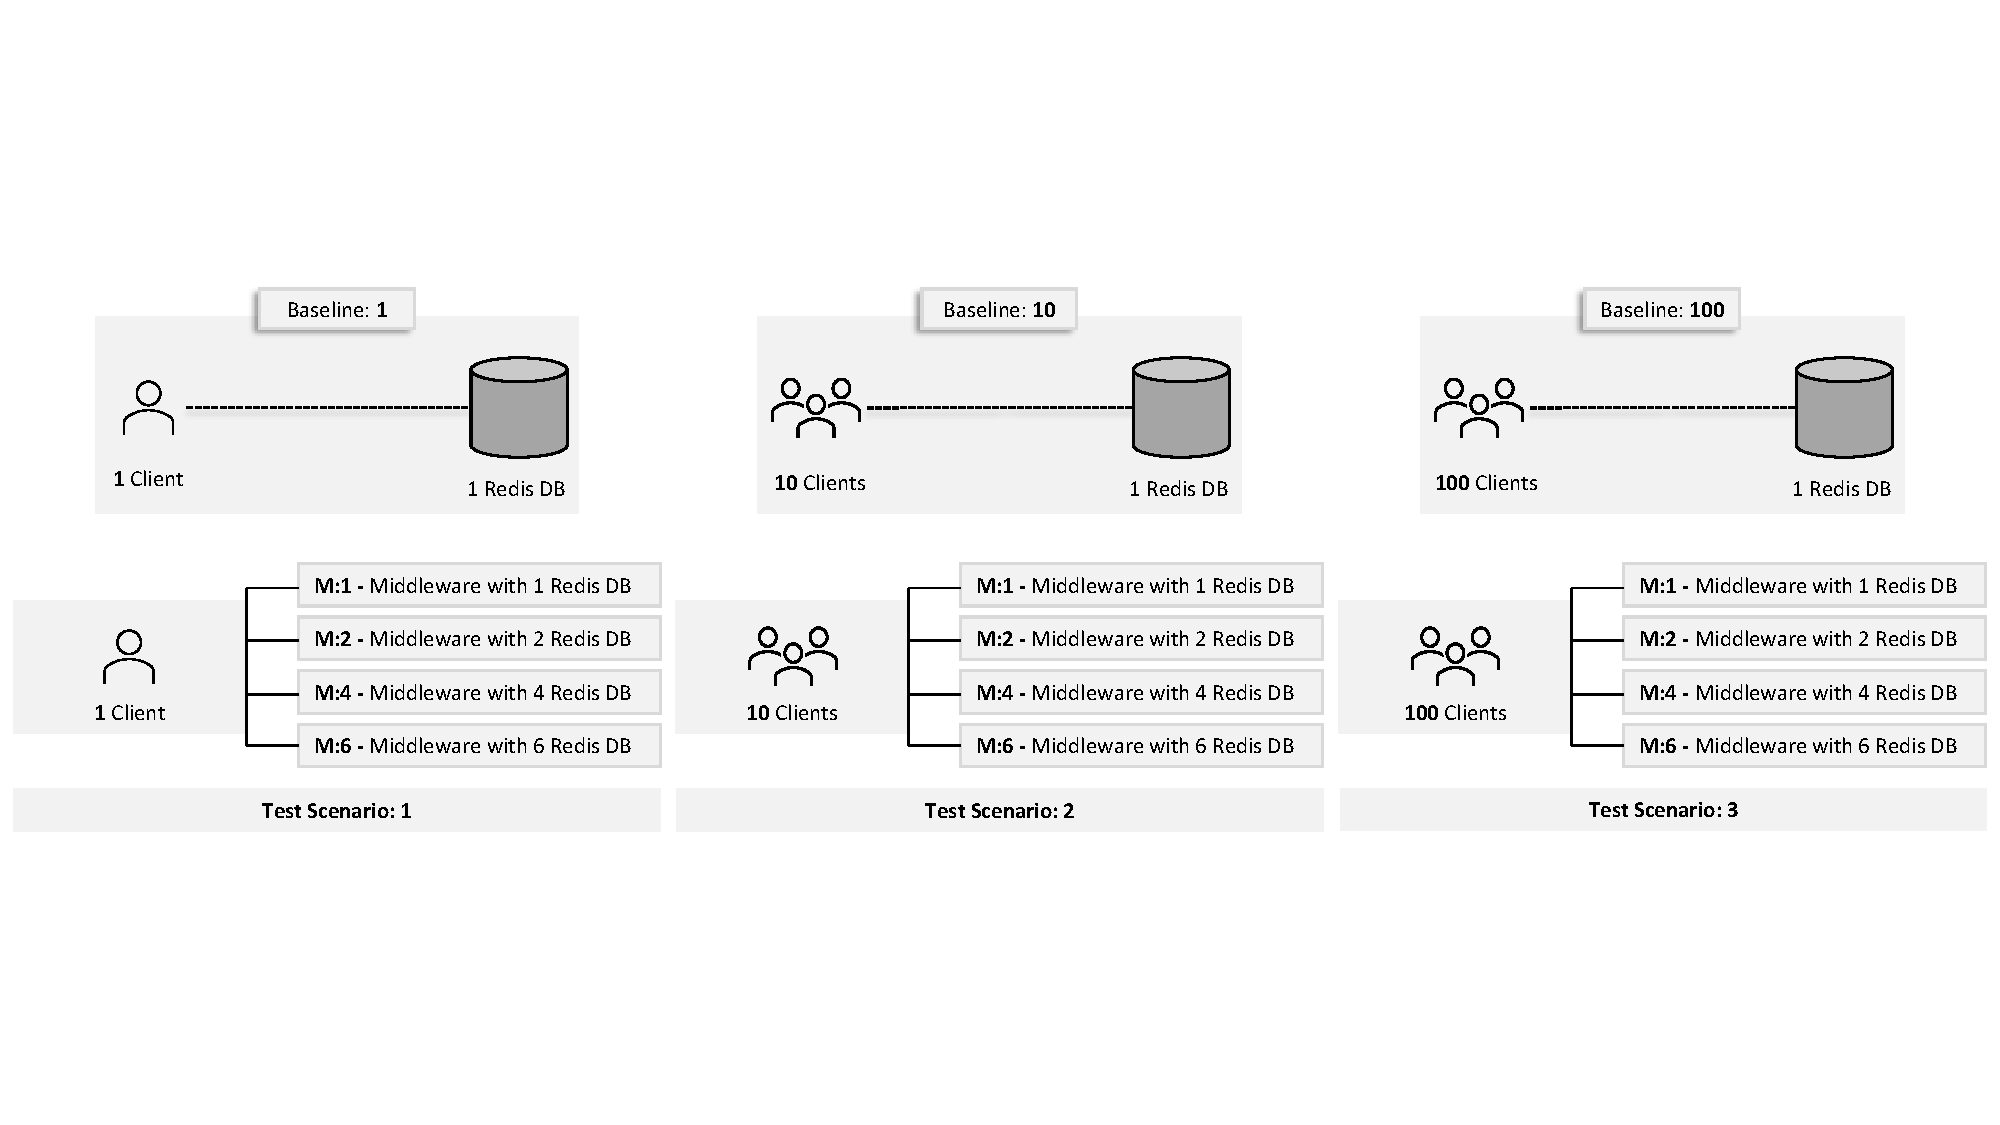
\includegraphics[width=\textwidth]{gfx/figures/Test_Scenario_Constant_Client_Load.pdf}}{\caption[Test scenarios for constant client-load]{Illustration of all test scenarios to measure and compare average throughput and average response time of the middleware relative to baseline and taking client-load variation into account for each scenario; DB: Database}\label{constant-client-load}}
\end{figure}

This approach assists in a more straightforward comparison of the impact that varying number of connected Redis databases to the middleware has on the performance under a constant workload over time. Moreover, this approach identifies the level of the client-load that causes the middleware to be overloaded and determines whether the middleware can handle additional clients. \\

\item \textbf{Gradually increasing client-load for the load-test execution:} \\

\noindent In this test condition, the client-load progressively increases throughout the load-testing phase for the baseline and for each middleware configuration. The number of clients, i.e., client-load starting with 1 client, grows at a spawning rate of 1 client every 2 seconds until a saturation point is reached. For the performance evaluation in this thesis, a maximum limit of 50 concurrent clients is considered for this test scenario. A visual representation of the test scenario under this specific condition is depicted in \cref{increasing-client-load}.

\begin{figure}[H]
             \ffigbox{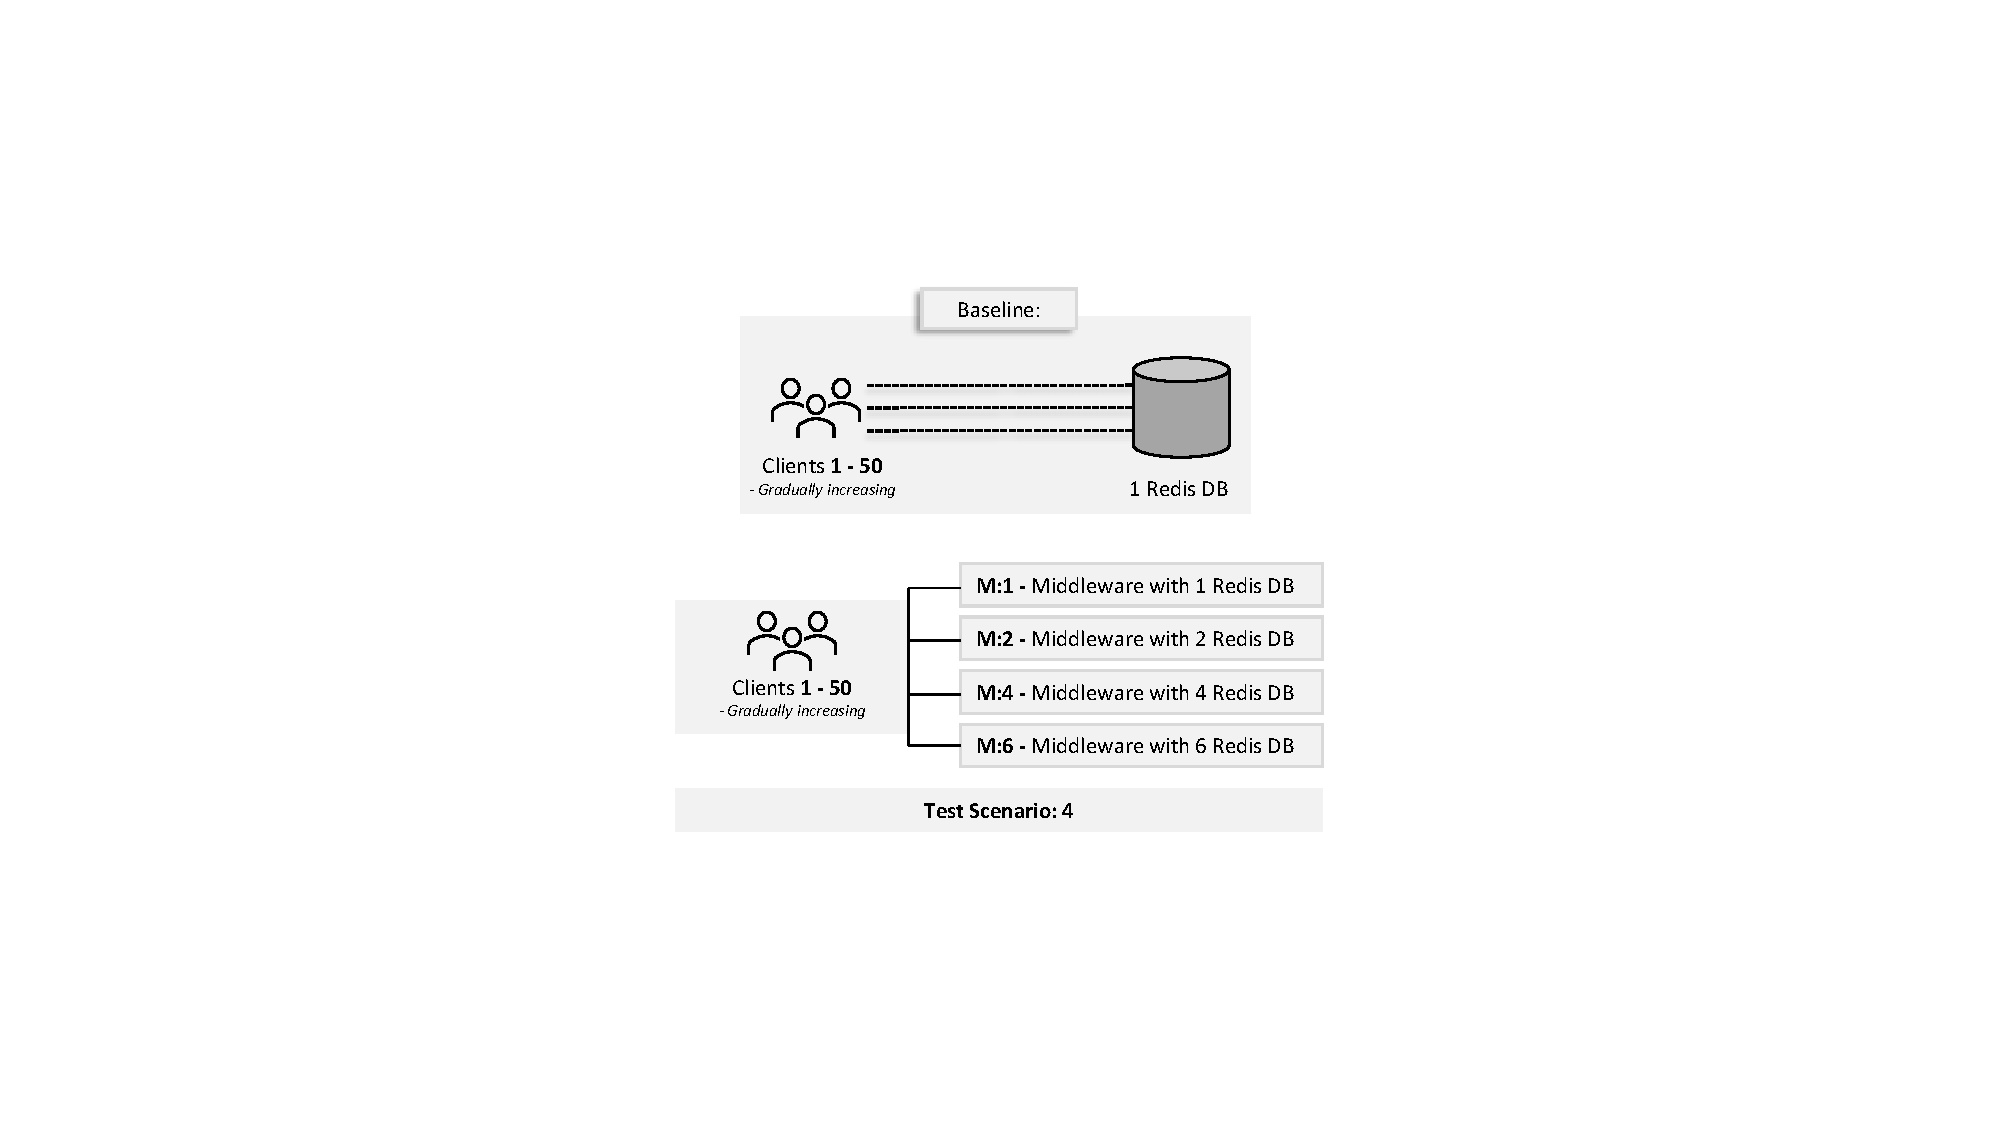
\includegraphics[width=\textwidth]{gfx/figures/Test_Scenario_Varying_Client_Load.pdf}}{\caption[Test scenarios for increasing client-load]{Illustration of test scenario with gradually increasing clients to measure and compare average throughput and response time of the middleware across different configurations, relative to baseline}\label{increasing-client-load}}
\end{figure}

\end{enumerate}


%***************************************************************************
%***************************************************************************
\section{Throughput and Response Time Analysis}
\label{throughputAnalysis}

Building upon the test conditions and the test scenarios defined in the subsection \ref{testScenario}, the performance of the middleware with respect to the established baseline, specifically in terms of average throughput and average response time, is analyzed and evaluated in this subsection. 

%***************************************************************************
%***************************************************************************
\subsection*{\textbf{Average Throughput}}

In the constant client-load condition, there are 3 test scenarios (Test Scenario: 1, Test Scenario: 2, and Test Scenario: 3) as illustrated in the \cref{constant-client-load}. The load-test execution for each test scenario with constant client-load is conducted for 3 minutes using the middleware configurations from the subsection \ref{config}. A warm-up time and cool-down time of 10 seconds each are excluded from the test execution time, accounting for system startup, process initialization, garbage collection, and system teardown. From the remaining 2 minutes and 40 seconds, only the test execution period of 1 minute is considered, where the system reaches a stable state. \\

\noindent In each test scenario, a baseline is established, where the client is connected to 1 Redis database and performs all the operations from the \cref{tab:workload}. All the operations are performed using the workloads $Dataset_{1}$ and $Dataset_{2}$ as defined in the subsection \ref{workloadBenchmark}. The custom workload is ready-heavy and write-heavy, resembling most real-world scenarios. The middleware’s behavior, when connected with 1, 2, 4, and 6 Redis databases, is evaluated in relation to the corresponding baseline for each scenario. For each client-load situation, the workload remains the same, i.e., all clients perform all operations using the same key-value pairs. This approach ensures that the middleware can handle all operations on identical key-value pairs. \\

%%%%%%%%%%%%
\noindent In \textbf{Test Scenario: 1} with a constant client-load of 1, the baseline's average throughput observed during the test execution ranges from approximately 95 to 100 Requests per Second (RPS). The findings also imply that the client’s average throughput, when operating with the middleware, remains stable between 45 and 60 RPS throughout the 1 minute of test execution, as depicted in the \cref{throughput_1_client}. \\

\begin{figure}[H]
             \ffigbox{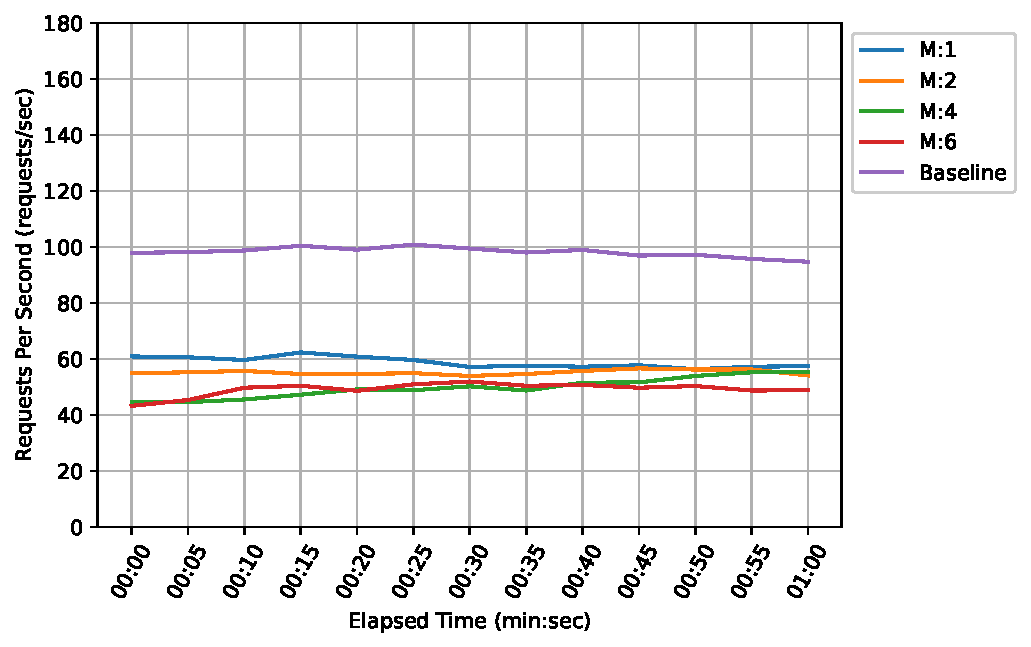
\includegraphics[width=\textwidth]{gfx/reports/throughput/throughput(rps)_1_Client.pdf}}{\caption{Average throughput measurement with 1 client-load (Test Scenario: 1)}\label{throughput_1_client}}
\end{figure}

\noindent When the middleware connected to 1 Redis database, the average throughput is around 58.4 RPS, which is marginally higher than other middleware configurations. However, when connected to 2 Redis databases, the average throughput of the middleware decreases to 53.7 RPS. This trend persists, with the middleware connected to 4 Redis databases exhibiting an average throughput of 50.6 RPS, and the middleware connected to 6 Redis databases yielding approximately 48.2 RPS. This clearly demonstrates that the throughput of the middleware connected to 1 Redis database (M:1) can handle approximately 10 more requests than that of the middleware connected to 6 Redis databases (M:6). \\

%%%%%%%%%%%%
\noindent In \textbf{Test Scenario: 2}, featuring a constant client-load of 10, the difference in observed throughput between the middleware with different configurations and the baseline remains consistent with the results observed under a client-load of 1. However, there is an increase in the middleware’s throughput as the client-load increases. This suggests that the middleware with a client-load of 1 is not saturated enough and can accommodate more concurrent clients. With the increased client-load of 10, the middleware can handle approximately 20 requests more every second than with the client-load of 1. Across all middleware configurations, the average throughput ranges from 70 to 75 RPS. But the trend for the middleware configurations, where additional Redis databases result in slightly lower throughput, persists in this case as well. The baseline’s average throughput in this case reaches approximately 153 RPS, which is a substantial difference from the prior test scenario. Likewise, the middleware demonstrates improved performance compared to the previous test scenario. However, the baseline configuration still facilitates higher throughput, as shown in the \cref{throughput_10_client}. \\

\begin{figure}[H]
             \ffigbox{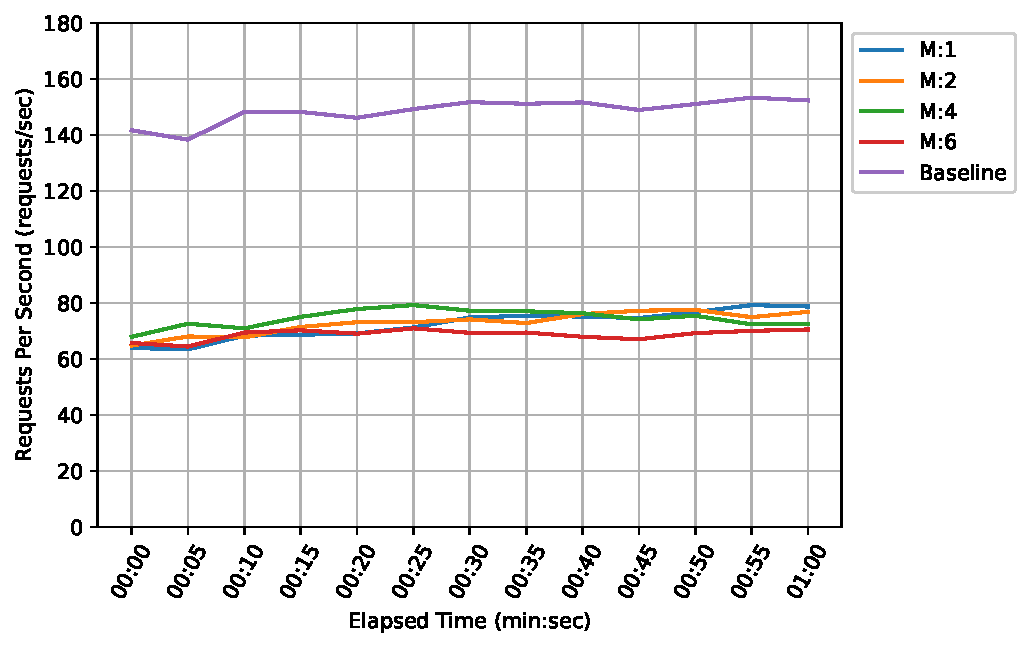
\includegraphics[width=\textwidth]{gfx/reports/throughput/throughput(rps)_10_Client.pdf}}{\caption{Average throughput measurement with 10 client-load (Test Scenario: 2)}\label{throughput_10_client}}
\end{figure}

\noindent In \textbf{Test Scenario: 3} with the client-load of 100, the average throughput of the baseline increases up to 170 RPS before starting to decrease, ultimately reaching around 160 RPS. This indicates that the baseline has reached its saturation point, with its computing resources being fully utilized. This is presumably due to the inability of 1 Redis database to handle the requests from 100 concurrent clients and execute operations with the same workload simultaneously. A deeper investigation of this behavior falls outside the scope of this thesis. However, the average throughput of all middleware configurations remains consistent at around 70 to 80 RPS, indicating that the middleware is saturated at this point. One of the potential reasons for the lack of throughput increase in the middleware could be potential increase in the response times, which will be discussed together with the evaluation of average response time.  \\

\noindent \cref{throughput_100_client} illustrates the variation of the middleware’s average throughput for each configuration with the client-load of 100, referencing to the baseline. \\

\begin{figure}[H]
             \ffigbox{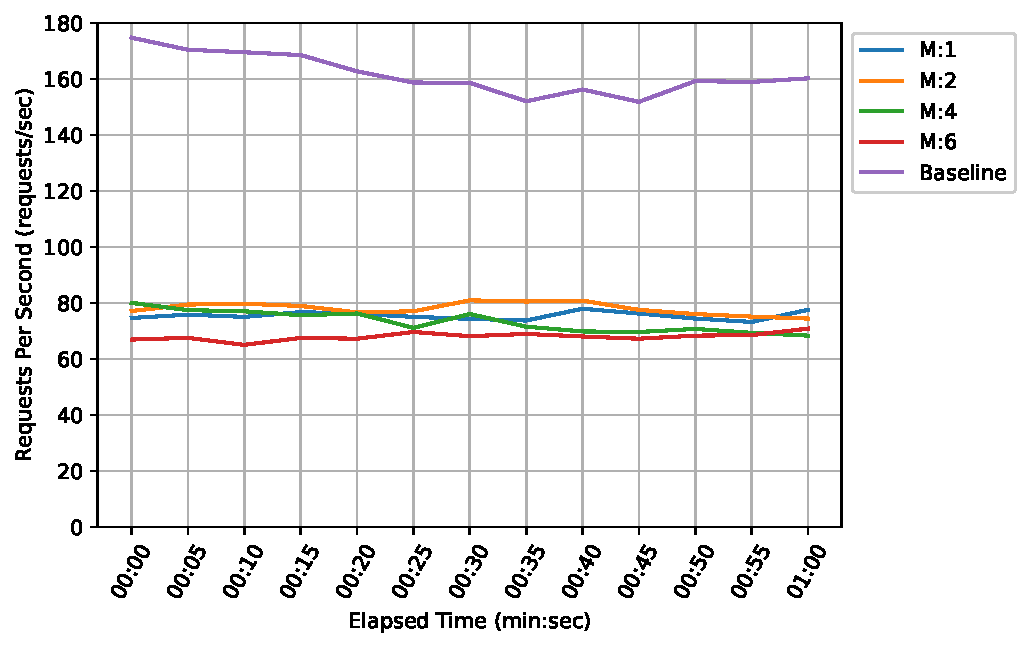
\includegraphics[width=\textwidth]{gfx/reports/throughput/throughput(rps)_100_Client.pdf}}{\caption{Average throughput measurement with 100 client-load (Test Scenario: 3)}\label{throughput_100_client}}
\end{figure}

\noindent \cref{tab:summary_constant_client} provides a summary of the average throughput of the baseline and the middleware observed in each given test scenario. The middleware’s throughput saturation point is at around 70 RPS from the given results. The average throughput initially increases and subsequently stabilizes when all the computing resources of the middleware are occupied. As the middleware is fully engaged in executing the operations for the corresponding requests, it becomes congested at a point and cannot accommodate more requests. \\

\begin{table} [H]
\centering
\begin{tabular}{@{} lcrrrrr @{}} % @{} removes white spaces
	\toprule
	Test Scenario & Client-load	&	Baseline	&	M:1	&	M:2  &		M:4  & 	M:6  \\
	%\tableheadlineL{Test} & \tableheadline{Client} & \tableheadline{Baseline} & \multirow{2}{*}{\spacedlowsmallcaps{M:1}} &  \multirow{2}{*}{\spacedlowsmallcaps{M:2}} &  \multirow{2}{*}{\spacedlowsmallcaps{M:4}} &  \multirow{2}{*}{\spacedlowsmallcaps{M:6}} \\ 
	%\tableheadlineL{Scenario}& \tableheadline{(N)*} & \tableheadline{(N)} & &  &  &  \\ 
	\midrule
	1	&	1 &	94.9 RPS	&	58.4 RPS	&	53.7 RPS	&	50.6 RPS	&	48.2 RPS \\
	2	&	10 &	153.0 RPS	&	76.3 RPS	&	74.6 RPS	&	71.5 RPS	&	70.7 RPS \\
	3	&	100 &	161.2 RPS	&	74.6 RPS	&	73.4 RPS	&	71.3 RPS	&	70.7 RPS \\
	\bottomrule
\end{tabular}
\caption[Average throughput measured during load-test execution with constant client-loads]{Average throughput measured during load-test execution with constant client-loads; Client-load*}
\label{tab:summary_constant_client}
\end{table}

\noindent An insightful evaluation of the middleware’s average throughput involves a comparison of its performance with gradually increasing client-load, which is defined as \textbf{Test Scenario: 4} in the subsection \ref{testScenario}. An overview of the observed results from the load-test execution of increasing client-load from 1 to 50 at a steady rate of 1 client every 2 seconds is shown in \cref{average_rps_50}. The outcomes in this test scenario are comparable to those in the test scenarios with constant client-load. \\

\begin{figure}[H]
             \ffigbox{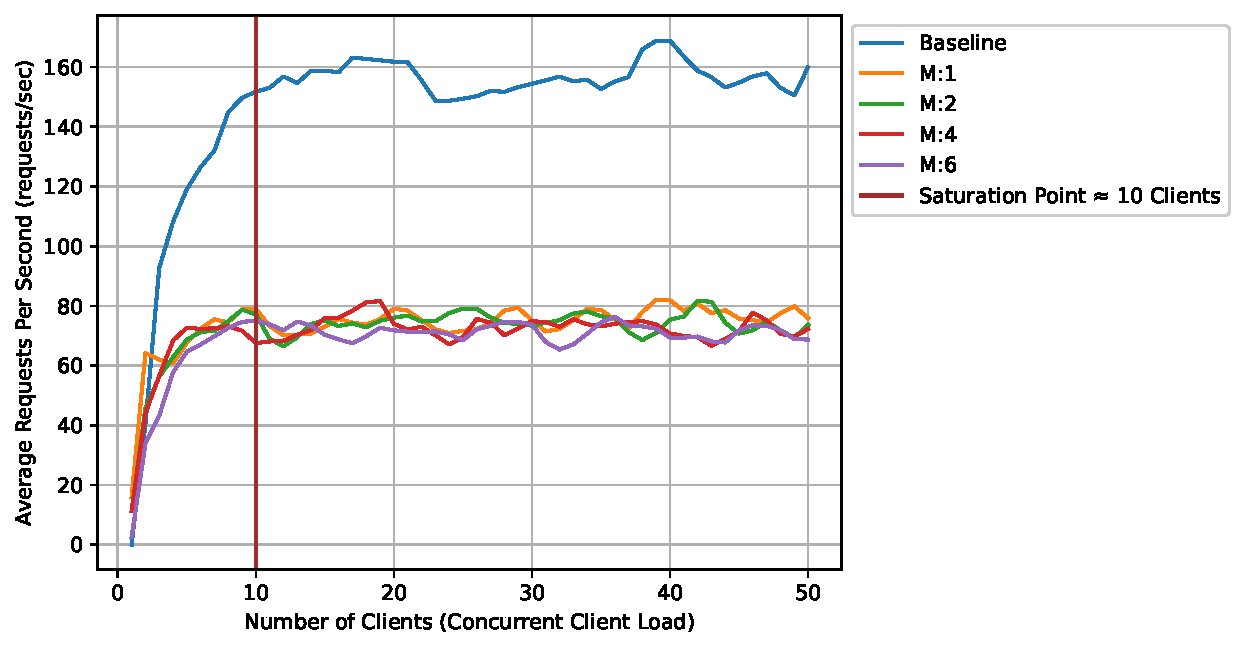
\includegraphics[width=\textwidth]{gfx/reports/throughput/average_rps_50.pdf}}{\caption{Average throughput with respect to increasing client-load ranging from 1 to 50 (Test Scenario: 4)}\label{average_rps_50}}
\end{figure}

\noindent The baseline without the middleware, i.e., the single Redis database, does not exhibit a stable and significant increase in the average throughput beyond the client-load of 10. From that point, the average throughput fluctuates and becomes unstable. Similarly, for the middleware with different configurations of the Redis databases, the average throughput increases with an increasing number of clients to 10. However, there is no notable improvement in average throughput beyond the client-load of 10. This suggests that both the baseline and the middleware with different configurations can be evaluated with the client-load ranging from 1 to 10, with 10 being the approximate saturation point. \cref{tab:summary_varying_client} presents the findings from this test scenario. \\

\begin{table} [H]
\centering
\begin{tabular}{@{} lcrrrrr @{}} % @{} removes white spaces
	\toprule
	Test Scenario & Client-load	&	Baseline	&	M:1	&	M:2  &		M:4  & 	M:6  \\
	%\tableheadlineL{Test} & \tableheadline{Client} & \tableheadline{Baseline} &  \multirow{2}{*}{\spacedlowsmallcaps{M:1}} &  \multirow{2}{*}{\spacedlowsmallcaps{M:2}} &  \multirow{2}{*}{\spacedlowsmallcaps{M:4}} &  \multirow{2}{*}{\spacedlowsmallcaps{M:6}} \\ 
	%\tableheadlineL{Scenario}& \tableheadline{Load} &  & &  &  &  \\ 
	\midrule
	4 & 1 to 50	&	155.5 RPS &	74.8 RPS	&	73.6 RPS	&	72.3 RPS	&	70.1 RPS \\
	\bottomrule
\end{tabular}
\caption[Average throughput measured during load-test execution with increasing client-load]{Overview of average throughput of the baseline and the middleware with steadily increasing number of clients from 1 to 50}
\label{tab:summary_varying_client}
\end{table}

\noindent The findings from the test execution with the client-load ranging from 1 to 10 is depicted in \cref{average_rps_10}, resulting in maximum throughput of \textbf{151.75 RPS} with the baseline and \textbf{80 RPS} with the middleware. The evaluation demonstrates a stable growth in the observed throughput of both the baseline and the middleware. However, it reveals that adding more Redis database instances to the middleware results in a slight degradation of its performance. This could be attributed to increased network latencies stemming from the additional communicating entities. As more databases are incorporated, greater communication overhead arises between the middleware and the databases. Moreover, a single middleware instance communicating with multiple Redis databases creates a bottleneck, as it must decompose all client requests into multiple sub-requests, dispatch them to the corresponding Redis databases, and retrieve the partial results. The middleware is then responsible for aggregating these results and returning them to the respective clients. This process consumes the middleware's processing resources, leaving insufficient resources available for handling other requests. Consequently, pending requests must wait for the middleware to become available, preventing the middleware from processing additional requests and achieving better throughput. A detailed discussion of these evaluations and their implications is provided in section \ref{ch:discussion}.\\

\begin{figure}[H]
             \ffigbox{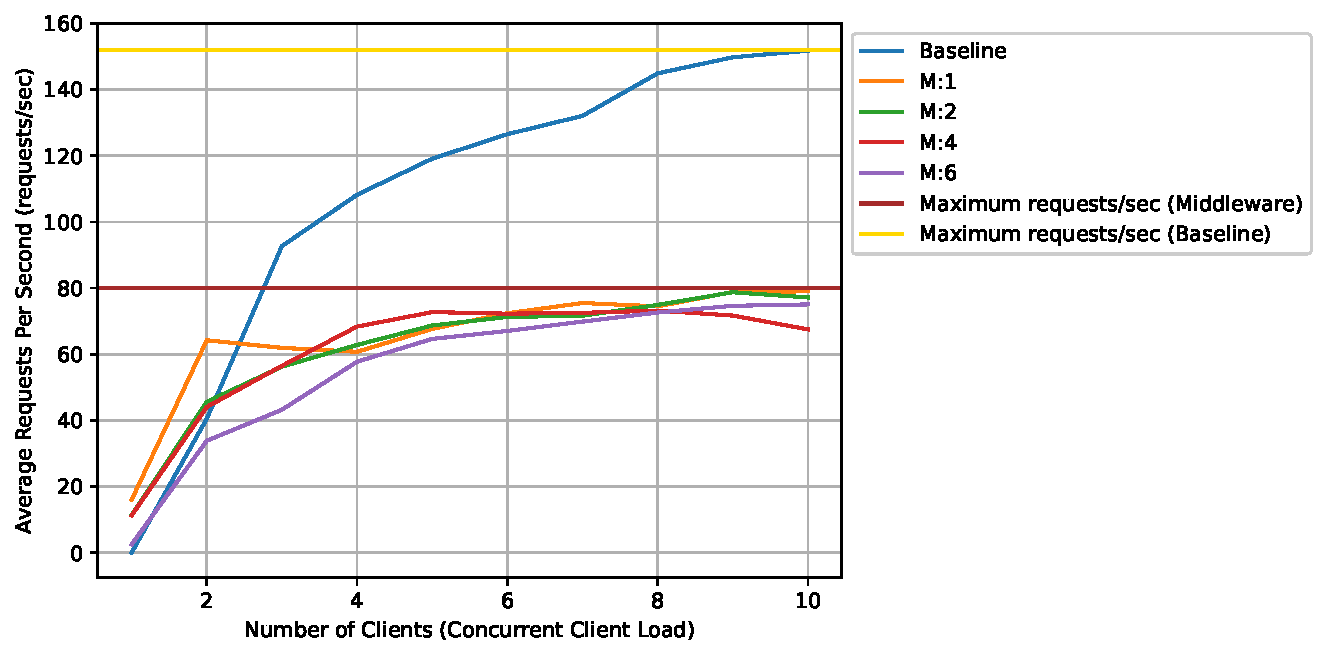
\includegraphics[width=\textwidth]{gfx/reports/throughput/average_rps_10.pdf}}{\caption{Average throughput with respect to increasing client-load ranging from 1 to 10}\label{average_rps_10}}
\end{figure}


%%%%%%%%%%%%
\subsection*{\textbf{Average Response Time}}

To measure the average response time of the middleware with different configurations, a progressively increasing client-load ranging from 1 to 50 is considered, as defined in \textbf{Test Scenario: 4} within subsection \ref{testScenario}. For the baseline, the average response time of a single Redis database connected to a single client is measured. As depicted in \cref{average_res_50}, the baseline exhibits a consistent and linear increase of the average response time, with the growing number of concurrent clients. The average response time begins at approximately 11.88 milliseconds (ms) for 1 client and peaks at around 94.48 ms for 50 concurrent clients, executing all operations ($set$, $get$, $get$-$range$, $delete$) with $Dataset_{1}$ and $Dataset_{2}$, as defined in subsection \ref{workloadBenchmark}. The observed response time for the baseline shows a linear growth of about 1.70 ms. \\

\noindent For assessing the average response time of the middleware as perceived by the connected client, it is essential to consider factors, directly or indirectly influencing the response time. These factors include:
\begin{itemize}
\item[-]	Processing time of the middleware (Service Time)
\item[-]	Internal response time of the associated Redis databases within the middleware
\item[-]	Waiting time of the middleware for the corresponding response (Wait Time)
\item[-]	Network latencies, i.e., the time delays caused by the network between the client and the middleware, as well as between the middleware and the associated Redis databases.
\end{itemize}

\begin{figure}[H]
             \ffigbox{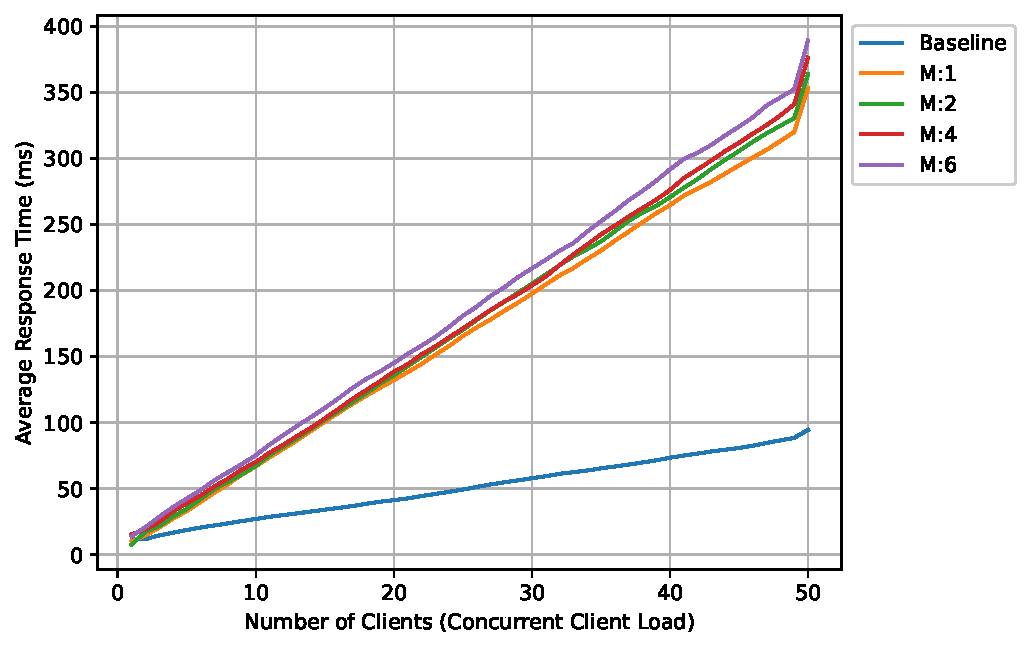
\includegraphics[width=\textwidth]{gfx/reports/response_time/avg_response_time_50.pdf}}{\caption{Average response time with respect to steadily increasing client-load from 1 to 50}\label{average_res_50}}
\end{figure}

\noindent Both network latencies and processing times are dynamic factors that change with time and scenarios, making it difficult to obtain concrete and accurate measurements. Due to these factors, the response time may include some noise and unintentional delays. Hence, the outcomes from the load-test executions should be considered approximate values. \cref{tab:response_time_average} states the observed average response times of the baseline and all the middleware configurations with constant client-load of 1, 10, and 100. 

\begin{table} [H]
\centering
\begin{tabular}{@{} lrrrrr @{}} % @{} removes white spaces
	\toprule
	 %\multirow{2}{*}{\spacedlowsmallcaps{Client-Load (N)}} & \multirow{2}{*}{\spacedlowsmallcaps{Baseline (N)}} & \multirow{2}{*}{\spacedlowsmallcaps{M:1}} &  \multirow{2}{*}{\spacedlowsmallcaps{M:2}} &  \multirow{2}{*}{\spacedlowsmallcaps{M:4}} &  \multirow{2}{*}{\spacedlowsmallcaps{M:6}} \\ 
	Client-load	&	Baseline	&	M:1	&	M:2  &		M:4  & 	M:6  \\
	\midrule
	1 &	10.46 ms	&	15.10 ms	&	16.47 ms	&	17.62 ms	&	18.63 ms \\
	10 &	40.33 ms	&	125.75 ms	&	128.57 ms &	134.42 ms	&	135.63 ms \\
	100 &	327.32 ms &	1297.37 ms &	 1353.55 ms &	1360.46 ms & 1372.55 ms \\
	\bottomrule
\end{tabular}
\caption{Observed average response time of the middleware and the baseline with different client-load}
\label{tab:response_time_average}
\end{table}

\noindent Considering the saturation point of 10 client-load, as per the evaluation of throughput of the baseline and the middleware, the observed response time behavior concerning the number of concurrent clients in the system is represented in \cref{average_res_10}.

\begin{figure}[H]
             \ffigbox{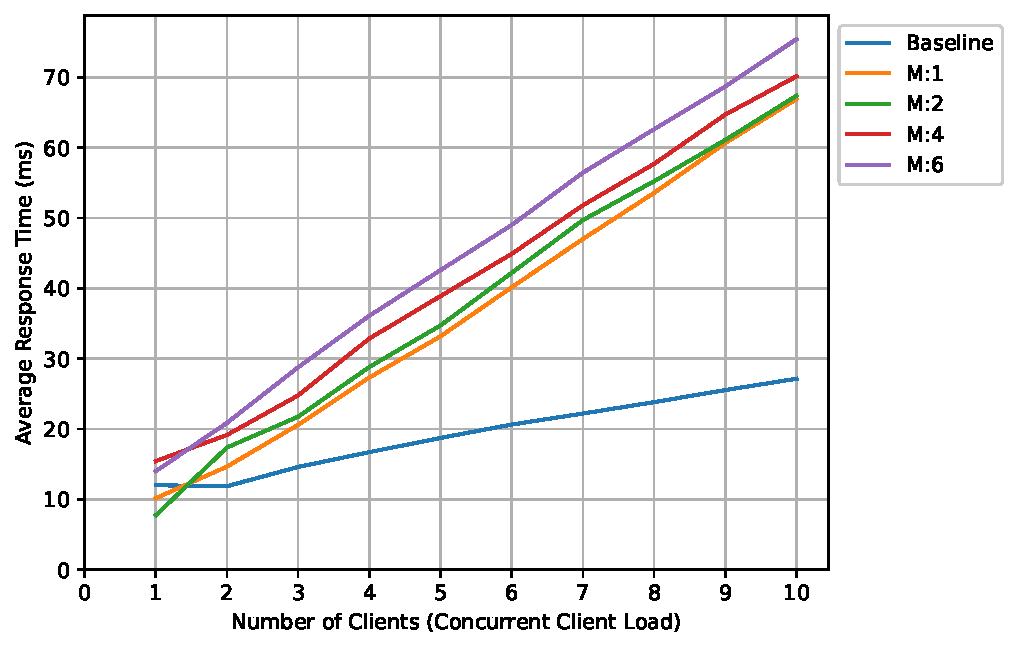
\includegraphics[width=\textwidth]{gfx/reports/response_time/avg_response_time_10.pdf}}{\caption{Average response time with respect to steadily increasing client-load from 1 to 10}\label{average_res_10}}
\end{figure}

\noindent Based on the evaluation, it can be concluded that the average response time of both the baseline and the middleware for all configurations increases linearly. The observed linear growth in the middleware’s response time with increasing number of concurrent clients from 1 to 10 is given in \cref{tab:linear_growth_rate}.

\begin{table} [H]
\centering
\begin{tabular}{@{} ccc @{}} % @{} removes white spaces
	\toprule
	 %\tableheadline{Middleware Configurations} & & \tableheadline{Linear Growth Rate (Response Time)} \\
	 Middleware Configurations & & Linear Growth Rate (Response Time) \\
	\midrule
	M:1 &	&	 $\approx$ 6.66 ms \\
	M:2 &	&	 $\approx$ 6.37 ms \\
	M:4 &	&	 $\approx$ 6.10 ms \\
	M:6 &	&	 $\approx$ 6.23 ms \\
	\bottomrule
\end{tabular}
\caption{Linear growth rate of the average response time observed in different middleware configurations}
\label{tab:linear_growth_rate}
\end{table}

\noindent To obtain meaningful comparisons between the middleware and the baseline, set and get operations involving single and multiple key-value pairs are thoroughly analyzed, focusing on a single client connected to one middleware instance, as illustrated in \cref{set_get_m1}, \cref{set_get_m2}, \cref{set_get_m4}, and \cref{set_get_m6}. The middleware with 1 Redis database (M:1), providing an interface to a single client, has an average response time of approximately 3.89 ms for storing or setting 1 key-value pair in the database, whereas it has an average response time of around 4.01 ms for retrieving the 1 key-value pair from the database. In the case of 1000 key-value pairs, M:1 has an average response time of around 41.85 ms for setting all the key-value pairs and 38.36 ms for retrieving all of them. The average response time observed in the baseline for setting 1 key-value pair is around 1.89 ms, while for getting 1 key-value pair, it is around 2.11 ms. Meanwhile, for the 1000 key-value pairs, the average response times for setting and getting multiple key-value pairs are around 24.03 ms and 21.91 ms, respectively, which is nearly half of the average response time observed from M:1. \\

\begin{figure}[H]
	\begin{floatrow}
             \ffigbox{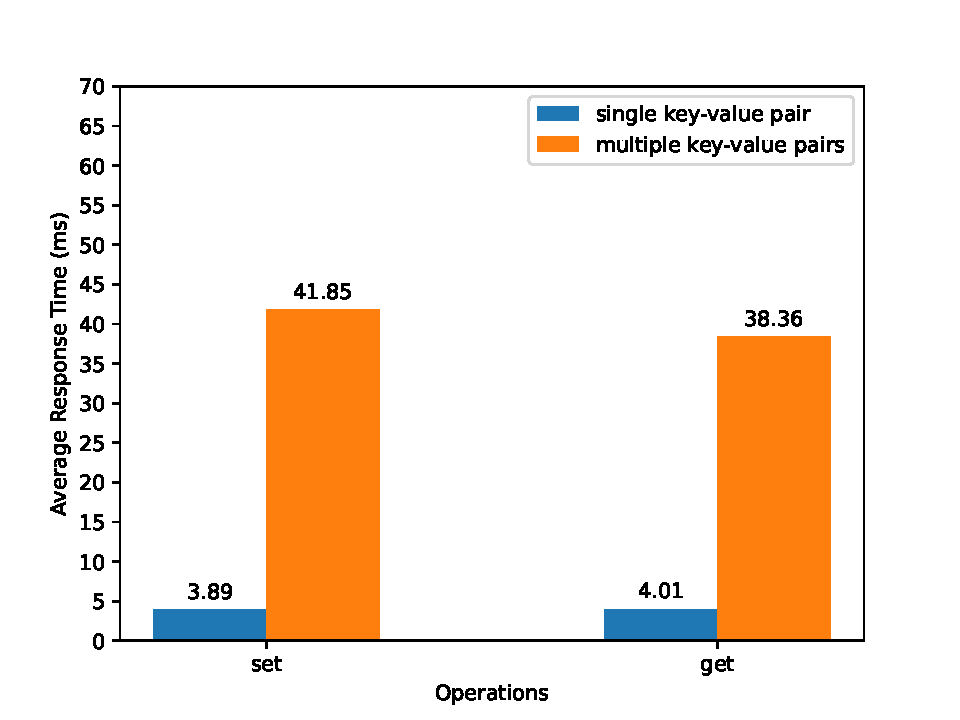
\includegraphics[scale = 0.5]{gfx/reports/response_time/set_get/set_get_1_Client_M-1.pdf}}{\caption{Set and Get operations with M:1}\label{set_get_m1}}
             \ffigbox{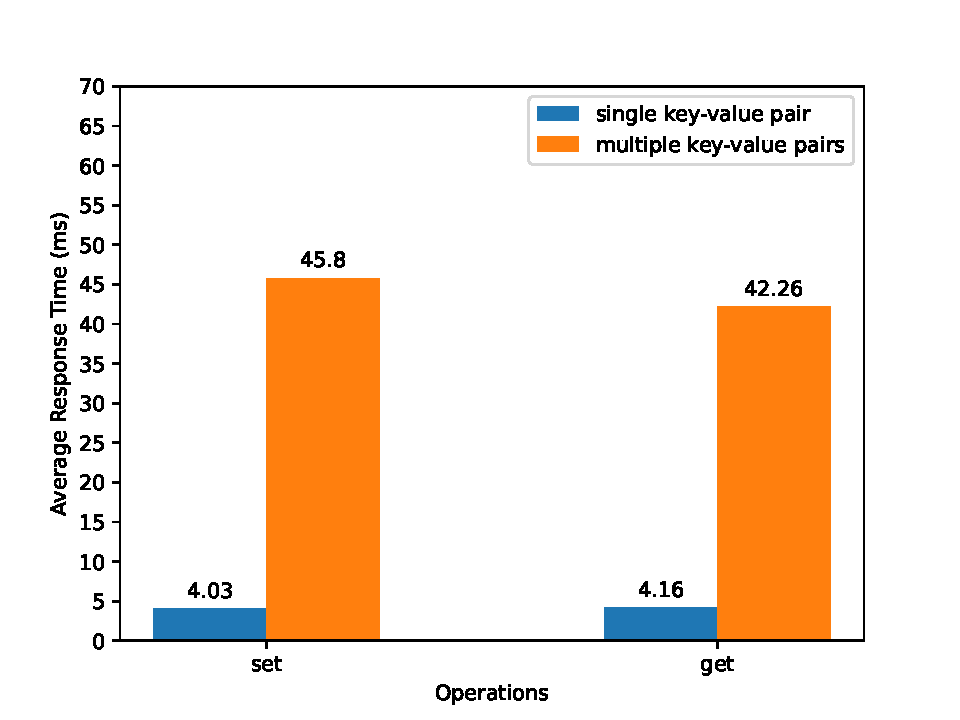
\includegraphics[scale = 0.5]{gfx/reports/response_time/set_get/set_get_1_Client_M-2.pdf}}{\caption{Set and Get operations with M:2}\label{set_get_m2}}
	\end{floatrow}
\end{figure}
\begin{figure}[H]
	\begin{floatrow}
             \ffigbox{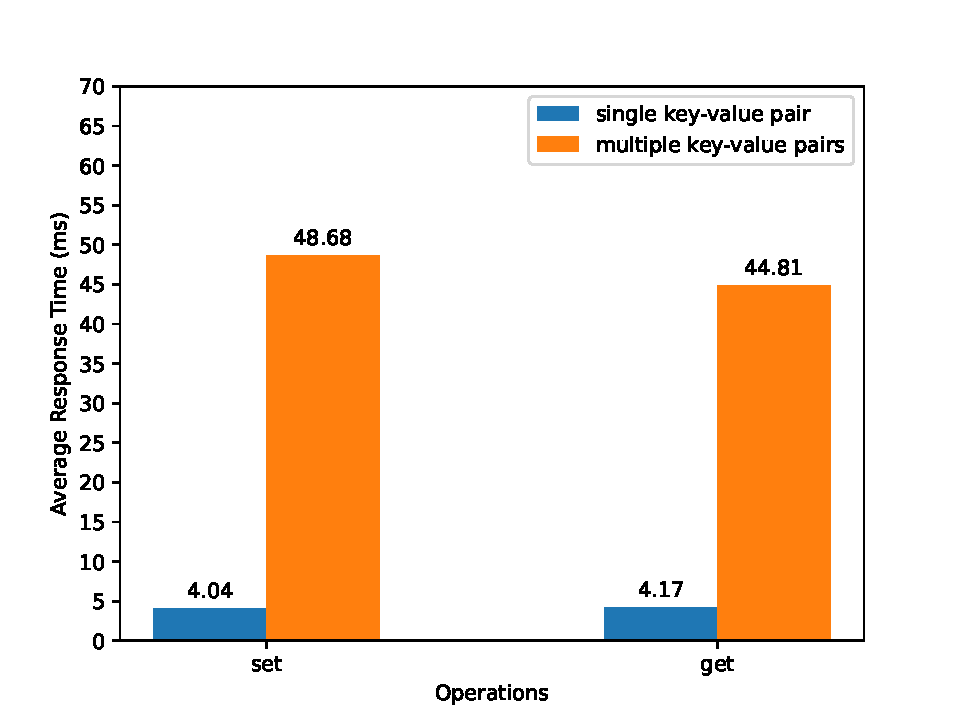
\includegraphics[scale = 0.5]{gfx/reports/response_time/set_get/set_get_1_Client_M-4.pdf}}{\caption{Set and Get operations with M:4}\label{set_get_m4}}
             \ffigbox{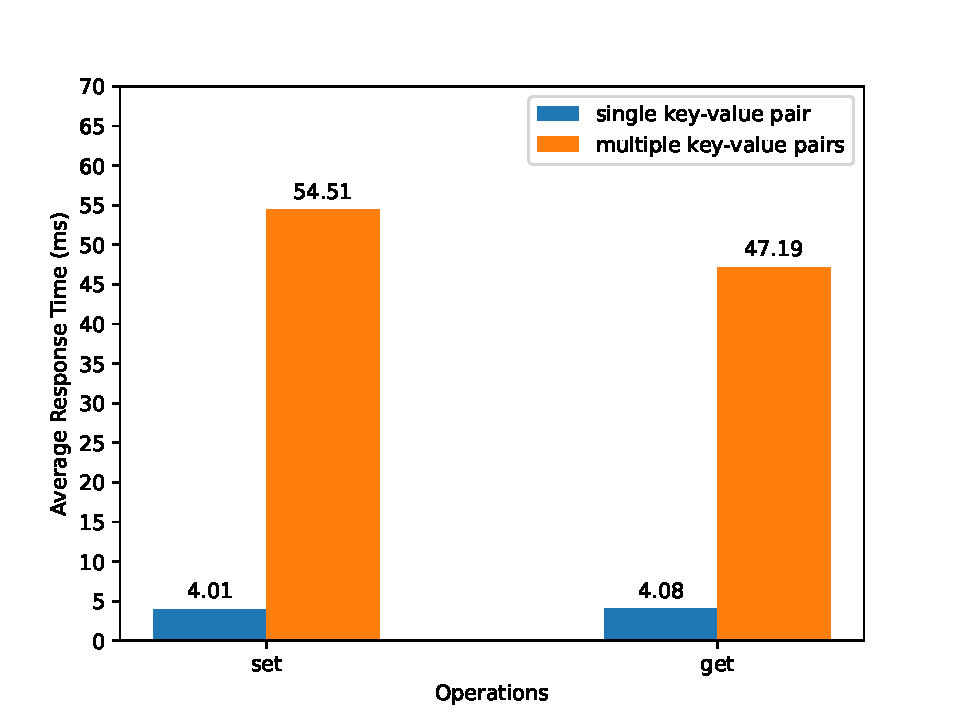
\includegraphics[scale = 0.5]{gfx/reports/response_time/set_get/set_get_1_Client_M-6.pdf}}{\caption{Set and Get operations with M:6}\label{set_get_m6}}
	\end{floatrow}
\end{figure}

\noindent Comparing the observed response times reveals a significant difference between setting and getting 1 key-value pair versus 1000 key-value pairs. This disparity can be attributed to the workload. In the baseline, setting and retrieving 1 key-value pair occurs sequentially, while for 1000 key-value pairs, a pipeline is created to queue all requests and a single bulk operation request is sent. In the middleware, 1 key-value pair is not sharded and is directly stored or fetched from the associated Redis database, whereas for 1000 key-value pairs, sharding is performed, which introduces processing overhead. Additionally, factors such as network latencies and communication overhead negatively impact the middleware's response time. \\

\begin{figure}[H]
             \ffigbox{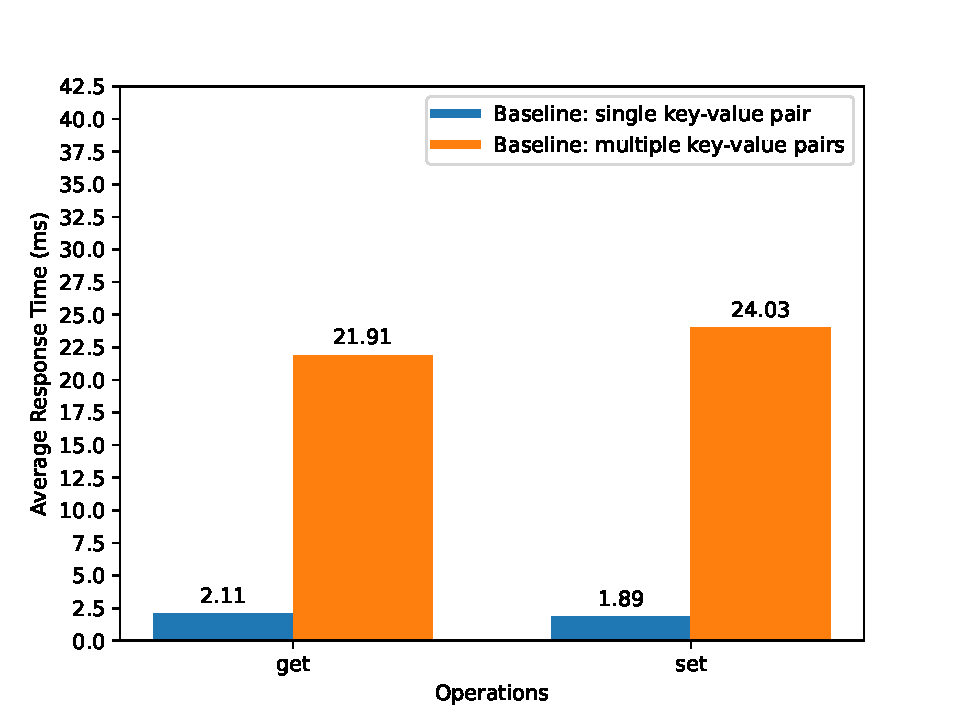
\includegraphics[scale = 0.5]{gfx/reports/response_time/set_get/set_get_baseline.pdf}}{\caption{Set and Get operations with Baseline}\label{set_get_baseline}}
\end{figure}
 
\noindent The difference between setting and getting 1 key-value pair in the baseline and the middleware should not be significant; however, the results indicate otherwise. This discrepancy can be attributed to the middleware introducing additional communication entities, which further increases processing overhead unless the middleware is carefully designed with concurrency features and optimized utilization of computing resources. A bottleneck also arises when using a single middleware instance to communicate with clients and all associated Redis databases. This is another reason for the slight degradation in the middleware's response time when more Redis databases are added. As more Redis databases are connected to a single middleware instance, the average response time also increases by 1 to 6 ms, as shown in \cref{set_get_m2} for M:2, \cref{set_get_m4} for M:4, and \cref{set_get_m6} for M:6. \\

\noindent For a more fine-grained evaluation, the average response time of the middleware is divided into two components:
\begin{itemize}
\item[-]	Internal response time from the connected databases within the middleware ($Internal\:DB$-$RT$)
\item[-]	$Service\:Time$ and $Wait\:Time$ for requests and responses
\end{itemize}
For the simplification of performance analysis, the average response time is considered as the total response time observed with the middleware. With this approach, the total $Response\:Time$ ($RT$) can be derived as: \\ 

$Total\:RT$ $\approx$ $Internal\:DB$-$RT$ + ($Service\:Time$ and $Wait\:Time$ ) \\

\noindent \cref{overview_rt} provides detailed information about the total response time, internal response time within the middleware, and the waiting and processing time of the middleware with various configurations. As observed in \cref{set_get_baseline} and the results outlined in \cref{overview_rt}, the $Internal\:DB$-$RT$ for set and get operations for a single key-value pair is smaller than the observed response time in the baseline. This difference can be attributed to the connection setup time of the Redis database in the baseline, while in the middleware, the connection to the Redis database is already established during the middleware's startup. However, the $Total\:RT$ of the middleware is slower than the baseline due to the $Service\:Time$ of the middleware for the requests and the $Wait\:Time$ of the responses from the associated databases. Consequently, this result indicates that the baseline is almost twice as responsive as the M:1 configuration. \\

\begin{table} [H]
\centering
\begin{tabular}{@{}llccr@{}} 
\toprule
     \multirow{2}{*}{Middleware} & \multirow{2}{*}{Requests} & \multirow{2}{*}{Total RT} & Internal  & Service Time and  \\
      & & & DB-RT & Wait Time  \\
    \midrule
    \multirow{7}{*}{M:1} & set\textunderscore single  & 3.9896 & 1.7717 & 2.2179  \\
    &	set\textunderscore multiple  & 41.8467  & 16.9528 & 24.8939  \\
    &	get\textunderscore single  & 4.0148  & 0.5548 & 3.4600  \\
    &	get\textunderscore multiple  & 38.3633 & 11.2019 & 27.1615    \\ 
    &	get\textunderscore range  & 7.9164   & 1.6844 & 6.2319 \\
    &	del\textunderscore single  & 4.0209 & 0.3221 & 3.6988  \\
    &	del\textunderscore multiple  & 6.9168  & 1.6909 & 5.2259   \\ \midrule

     \multirow{7}{*}{M:2} & set\textunderscore single  & 4.0261 & 1.7490 & 2.277  \\
    &	set\textunderscore multiple  & 45.7991  & 19.1634 & 26.6358   \\
    &	get\textunderscore single  & 4.1628  & 0.5383 & 3.6245  \\
    &	get\textunderscore multiple  & 42.259  & 12.4283 & 29.8307     \\ 
    &	get\textunderscore range  & 8.8411   & 2.7823 & 6.0588 \\
    &	del\textunderscore single  & 4.1352  & 0.3929 & 3.7423   \\
    &	del\textunderscore multiple  & 7.6919  & 2.1648 & 5.5271    \\ \midrule
    
     \multirow{7}{*}{M:4} & set\textunderscore single  & 4.0353		& 	1.7843		&	2.2510 \\
    &	set\textunderscore multiple  &  48.6758	&	20.7641	&	27.9117 \\
    &	get\textunderscore single  & 	4.1707		& 	0.4332		&	3.7375 \\
    &	get\textunderscore multiple  &		44.8088	&	 14.1521	&	30.6568 \\ 
    &	get\textunderscore range  & 	 9.8087		&	 3.6182		&	6.1904 \\
    &	del\textunderscore single  & 	4.0891		& 	0.3047		&	3.7844 \\
    &	del\textunderscore multiple  & 8.6419		& 	3.221		& 	5.4208 \\ \midrule

     \multirow{7}{*}{M:6} & set\textunderscore single  &	4.0051 & 	1.7750 	& 2.2301		\\
    &	set\textunderscore multiple  &		54.5115 	& 	22.8808 	& 	31.6307		\\
    &	get\textunderscore single &	4.0775 	& 	0.4649 	& 	3.6126			\\
    &	get\textunderscore multiple  &		47.1893 	& 15.4793 	& 	31.7100		\\
    &	get\textunderscore range   &	11.2084	 & 	3.7737 	& 	7.4347		\\
    &	del\textunderscore single  &	4.1074 	& 	0.1915 	&	 3.9160		\\
    &	del\textunderscore multiple  &		9.8391 	& 	3.9923 	& 	5.8468		\\
 	\bottomrule
\end{tabular}
\caption[Comprehensive overview of average response time and processing overhead of middleware]{Comprehensive overview of average response time and processing overhead of the system with a single client connected to the middleware}
\label{overview_rt}
\end{table}

%%%%%%%%%%%%
\section{Data Distribution Analysis}
\label{dataDistribution}

This subsection provides a brief evaluation of the middleware's consistent hash sharding approach in achieving efficient and uniform data distribution among Redis databases. \\

\noindent The middleware employs consistent hashing for sharding large datasets, which ensures that the load is evenly distributed among the database nodes. Moreover, this approach guarantees that adding a new database node does not necessitate rehashing all data items \cite{1372064}. However, the addition and removal of database nodes in the system are beyond the scope of this thesis. In this section, a synthetic workload of 100 and 1000 key-value pairs as mentioned in the subsection \ref{workloadBenchmark}, is utilized to assess the data distribution across Redis databases using the consistent hashing approach. \\

\noindent The test executions employ middleware configurations, M:2 (2 shards), M:4 (4 shards), and M:6 (6 shards), as detailed in the subsection \ref{config}. The middleware with 1 Redis database (1 shard), i.e., M:1 is excluded from this test, as data distribution is not applicable with a 1 shard and all data is stored in 1 Redis database node. The ideal data distribution across all Redis databases would involve each database having an equal number of key-value pairs. However, achieving perfect data distribution and maintaining an equal number of key-value pairs in each Redis database is challenging. \\

\noindent In the middleware connected to 2 Redis databases (M:2), ideal data distribution for 100 key-value pairs would involve splitting them evenly, with 50 allocated to each Redis database. Similarly, for 1000 key-value pairs, each of the 2 Redis databases should store 500 key-value pairs. The middleware distributes 100 key-value pairs as follows: 61 in the first Redis database and 39 in the second. Although not perfect, the difference of these 22 key-value pairs is not substantial. Compared to the ideal distribution of 50 key-value pairs each, the first Redis database stores 11 more, while the second stores 11 fewer. For 1000 key-value pairs, the distribution results in 526 stored in the first Redis database and 474 in the second. These findings are illustrated in \cref{data_2_db}. \\

\noindent The middleware with 4 Redis databases (M:4) distributes the 100 key-value pairs as follows: 32 in the first Redis database node, 23 in the second, 30 in the third, and 15 in the fourth. Ideally, each database node should have 25 key-value pairs. However, the current data distribution ensures that no database experiences a data hotspot, as a maximum of only 32 key-value pairs are allocated to a single Redis database. This data distribution trend continues for 1000 key-value pairs, where a maximum of 291 key-value pairs are assigned to a single Redis database. The detailed result of data distribution in M:4 is illustrated in \cref{data_4_db}. \\

\noindent Data distribution in the middleware with 6 Redis databases (M:6) appears more uniform compared to previous middleware configurations. For 100 key-value pairs, the data is divided among the 6 databases or shards, with an ideal scenario of approximately 16 to 17 key-value pairs in a single database. For 1000 key-value pairs, the ideal distribution would be 166 to 167 key-value pairs per database. \cref{data_6_db} presents the optimal data distribution results achieved by M:6.

\begin{figure} [H]
    \centering
    \begin{subfigure}[b]{0.45\textwidth}
    \centering
    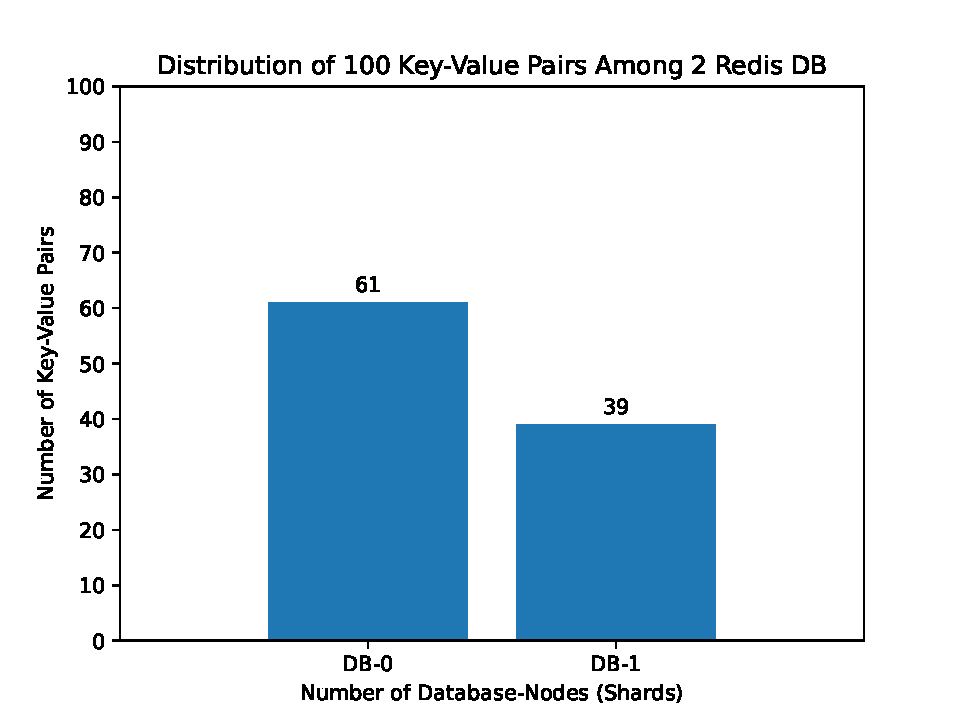
\includegraphics[width=\textwidth]{gfx/reports/data_distribution/2_DB/distribution-100.pdf}
    \end{subfigure}
    \begin{subfigure}[b]{0.45\textwidth}
    \centering
    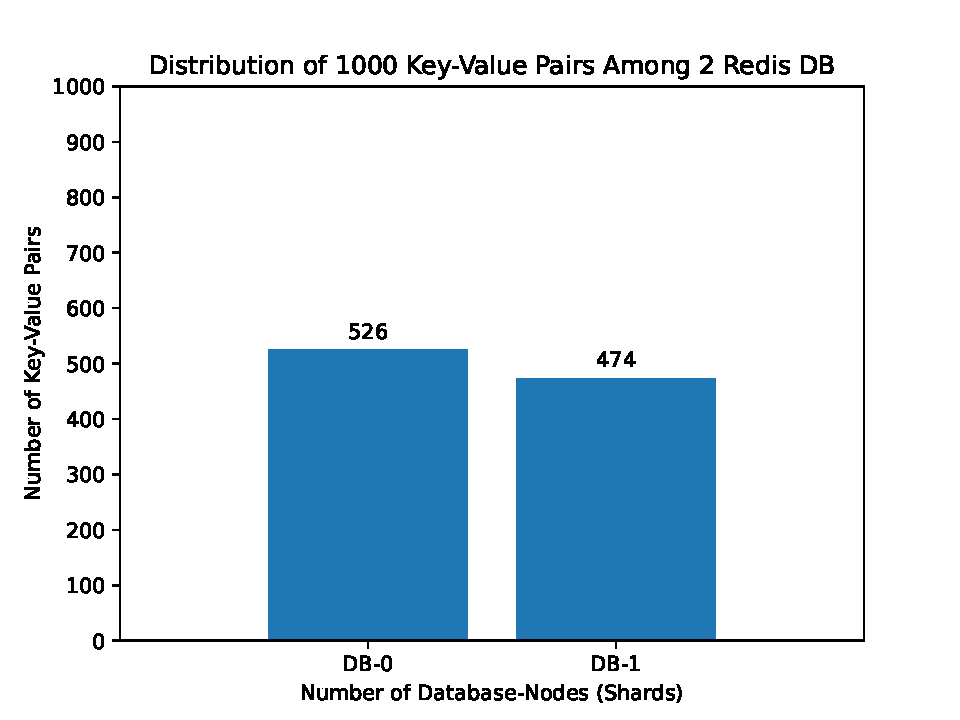
\includegraphics[width=\textwidth]{gfx/reports/data_distribution/2_DB/distribution-1000.pdf}
    \end{subfigure}
    \caption{Data distribution among 2 Redis databases (2 Shards)}
    \label{data_2_db}
\end{figure}

\begin{figure} [H]
    \centering
    \begin{subfigure}[b]{0.45\textwidth}
    \centering
    
\includegraphics[width=\textwidth]{gfx/reports/data_distribution/4_DB/distribution-100.pdf}
    \end{subfigure}
    \begin{subfigure}[b]{0.45\textwidth}
    \centering
    
\includegraphics[width=\textwidth]{gfx/reports/data_distribution/4_DB/distribution-1000.pdf}
    \end{subfigure}
    \caption{Data distribution among 4 Redis databases (4 Shards)}
    \label{data_4_db}
\end{figure}

\begin{figure} [H]
    \centering
    \begin{subfigure}[b]{0.45\textwidth}
    \centering
    
\includegraphics[width=\textwidth]{gfx/reports/data_distribution/6_DB/distribution-100.pdf}
    \end{subfigure}
    \begin{subfigure}[b]{0.45\textwidth}
    \centering
    
\includegraphics[width=\textwidth]{gfx/reports/data_distribution/6_DB/distribution-1000.pdf}
    \end{subfigure}
    \caption{Data distribution among 6 Redis databases (6 Shards)}
    \label{data_6_db}
\end{figure}








\iftoggle{parts}{
	\cleardoublepage
	\ctparttext{After the evaluation, we further discuss the results and give an outlook. In addition, we finish this work with conclusions.}
	\part{Discussion and Conclusions}
}{}
% !TeX root = ../Thesis.tex

%************************************************
\chapter{Discussion}\label{ch:discussion} % $\mathbb{ZNR}$
%************************************************
\section{Implications of Middleware-assisted Sharded Distributed Databases}
To address the three research questions introduced in chapter \ref{ch:introduction}, this thesis undertook the implementation and evaluation of a prototype middleware system that enabled sharding in databases, thereby creating a system of sharded distributed databases. The middleware's performance was assessed in terms of throughput, response time, and data distribution. This analysis identified several design-related limitations of the middleware. Despite these shortcomings and challenges, it delivered acceptable results, which leads to the conclusion that carefully designed sharded distributed databases have the potential to enhance the scalability of centralized databases. \\

\noindent From the load-test results presented in chapter \ref{evaluation}, the prototype of middleware designed for sharding exhibited acceptable performance in terms of system throughput. Upon further examination, it was determined that the middleware had limitations in managing multiple client requests due to its synchronous behavior. Each request had to wait for completion, occupying computing resources without utilizing them for other requests. During bulk read and write operations, the middleware experienced substantial high waiting times to receive results from the associated Redis databases. Consequently, the middleware's computing resources were engaged, but the process remained idle while waiting for responses from the Redis databases. As a single synchronous interface, the middleware was responsible for handling numerous client requests and orchestrating data management across multiple Redis databases. This also suggested the presence of a single bottleneck in the system, hindering optimal throughput. Despite these limitations, the middleware managed to achieve an average throughput of 80 Requests Per Second (RPS) when utilizing 6 Redis database instances, each containing 1 shard. This performance is considered acceptable considering the design goals of the middleware, as it was originally created as a single instance for communication and all operations were executed synchronously. There was no provision for the parallel execution of requests or concurrent computations to reduce the complexities of concurrency control and synchronization within the middleware. The primary objective was to implement a sharding approach using a middleware prototype to enable a functioning distributed database system, assess its performance, and identify challenges encountered during implementation. \\

\noindent Regarding response time, it was evident that the middleware connected to multiple Redis databases exhibited higher average response time compared to the baseline configuration of a single Redis database. When the middleware connected with multiple Redis databases was employed to synchronize data sharding and distribution, added network latencies arose due to the increased number of communication entities.The findings from the test execution indicated that the average response time observed for a single client connected to the middleware with six Redis database instance was approximately 9 milliseconds (ms) higher than that of the baseline, which consisted of a single client connected to one Redis database. This difference is reasonable given that the baseline involved only two communicating entities, while the middleware-assisted sharded distributed database system encompassed three and resulted in increased network latencies. When additional concurrent clients were connected, the middleware's average response time also exhibited a linear increase, which was an expected behavior due to the overloading of a single instance of middleware for handling multiple concurrent requests. \\

\noindent In terms of data distribution, the consistent hashing approach employing virtual nodes demonstrated effective data distribution. Test and evaluations in chapter \ref{evaluation}, which involved running the middleware with varying numbers of Redis databases and shards, indicated that the middleware successfully distributed 1000 key-value pairs across six Redis databases, achieving near-uniform data distribution without the risk of data hotspots. The evaluation showed a maximum of 183 key-value pairs assigned to one database and a minimum of 154 assigned to another, resulting in a maximum difference of merely 29 key-value pairs. \\

\noindent Considering the aforementioned findings and results, it can be concluded that the system of middleware-assisted sharded distributed databases leads to effective data distribution, which addresses the issue of overloaded single centralized databases. The middleware system adapts proficiently to multiple database node configurations, with each node containing a single shard. However, the evaluations of this thesis suggest that sharding introduces several challenges, including processing overhead in data and request distribution, compilation of partial results, and synchronization overhead across multiple database servers. Thus, sharded distributed databases should be suitably designed and optimized for peak performance, encompassing both throughput and response time.



%************************************************
\section{Limitations and Future Work}

% !TeX root = ../Thesis.tex

%************************************************
\chapter{Conclusion}\label{ch:conclusion}
%************************************************
%%\glsresetall % Resets all acronyms to not used
In conclusion, this thesis investigated the performance of middleware-assisted sharded distributed databases in comparison to the baseline using a single centralized database, focusing on throughput, response time, and data distribution. By designing and implementing a middleware prototype using consistent hashing with virtual nodes, the thesis examined the key factors influencing performance and addressed the challenges and bottlenecks encountered during the implementation. The results demonstrated that, despite certain limitations, sharded distributed databases supported by a middleware achieve effective data distribution while adapting to various database node and shard configurations and can enhance scalability when designed and implemented meticulously. Future work should tackle bottlenecks and limitations of the implemented prototype of middleware-assisted sharded distributed databases, such as single-instance middleware and synchronous request processing. Incorporating multi-instance middleware architecture, asynchronous processing, support for running different queries or requests in parallel across associated databases with concurrency control mechanisms within the middleware, and adaptability to distinct types of databases would significantly enhance the middleware's functionalities. Hence, this thesis has successfully examined a middleware prototype for sharding in databases, providing valuable insights and paving the way for future works aimed at enhancing the efficiency and scalability of sharded distributed databases.
% ********************************************************************
% Backmatter
%*******************************************************
\iftoggle{parts}{}{
	\addtocontents{toc}{\protect\vspace{\beforebibskip}} % add space between main chapters and appendix if we do not use parts
}
\appendix
%\renewcommand{\thechapter}{\alph{chapter}}
\cleardoublepage
\iftoggle{parts}{
	\part{Appendix}
}{}

% !TeX root = ../Thesis.tex

%********************************************************************
% Some Proof (Appendix)
%*******************************************************
% If problems with the headers: get headings in appendix etc. right
\markboth{\spacedlowsmallcaps{Appendix}}{\spacedlowsmallcaps{Appendix}}
\chapter{Appendices}\label{ch:appendices}
%%%%\glsresetall % Resets all acronyms to not used

\section{Experimental Data and Implementation Details}

\section{Detailed Performance Results}



%********************************************************************
% Other Stuff in the Back
%*******************************************************
\iftoggle{parts}{
	\include{Parts/BackMatter}
}{}
\cleardoublepage\include{FrontBackmatter/Bibliography}
\iftoggle{phd}{
	%\cleardoublepage\include{FrontBackmatter/CurriculumVitae} % not required in final submission
	\cleardoublepage\include{FrontBackmatter/DeclarationPhD}
}{
	\cleardoublepage\include{FrontBackmatter/Declaration}
}
%\cleardoublepage\include{FrontBackmatter/Colophon}
% ********************************************************************
% Game Over: Restore, Restart, or Quit?
%*******************************************************
\end{document}
% ********************************************************************
